\documentclass{article}
\usepackage{amsmath, amsthm, amssymb, amsfonts, graphicx, color}
\usepackage{mathtools}
\usepackage{hyperref}
%\renewcommand{\rmdefault}{ppl}
%\usepackage[small, euler-digits]{eulervm}

\newcommand{\td}[2]{\frac{d{#1}}{d{#2}}}
\newcommand{\pd}[2]{\frac{\partial{#1}}{\partial{#2}}}
\newcommand{\cvar}[1]{\mathrm{char}_\alpha(#1)}
\newcommand{\cce}{\subset\subset}
\newcommand{\fint}{\mbox{--}\mkern-16mu\int}
\DeclarePairedDelimiter\norm{\lVert}{\rVert}
\DeclareMathOperator*{\esssup}{ess\,sup}
\DeclareMathOperator*{\Int}{Int}
\DeclareMathOperator{\dive}{div}

\theoremstyle{plain}
\newtheorem{thm}{Theorem}
\numberwithin{thm}{section}

\theoremstyle{plain}
\newtheorem{prop}{Proposition}
\numberwithin{prop}{section}

\theoremstyle{definition}
\newtheorem{defn}{Definition}
\numberwithin{defn}{section}

\theoremstyle{remark}
\newtheorem*{rem}{Remark}

\newtheorem*{cor}{Corollary}

\numberwithin{equation}{section}
\begin{document}
\title{Partial Differential Equations\\A Course by Prof. A. K. Nandakumaran}
\author{Amey Joshi}
\date{07-Aug-2018}
\maketitle

\section{Notation}\label{s1}
A point $x = (x_1, \ldots, x_n)$ will usually be a point in $\mathbb{R}^n$. By default, all vectors 
are column vectors. The set of natural numbers will include $0$. If $\alpha = (\alpha_1, \ldots, 
\alpha_n)$, where $\alpha_i$, for $1 \le i \le n$ are integers then the symbol $|\alpha| = \alpha_1 + 
\cdots + \alpha_n$. $U$ is usually a domain (that is, an open set) in $\mathbb{R}^n$. The symbol 
$D^\alpha$ is defined as
\begin{equation}\label{s1e1}
D^\alpha = \frac{\partial^{|\alpha|}}{\partial x_1^{\alpha_1}\cdots\partial x_n^{\alpha^n}}.
\end{equation}
We define
\begin{equation}\label{s1e2}
D^0f = f.
\end{equation}
If $e_i \in \mathbb{R}^n$ is the standard basis of the vector space $\mathbb{R}^n$ then
\[
D^{e_i}f = \pd{f}{x_i},
\]
where $f: \mathbb{R}^n \rightarrow \mathbb{R}$ is a function differentiable in a certain $U$. 
Using this notation, the gradient in $n$ dimensions is
\begin{equation}\label{s1e3}
Df = (D^{e_1}f, \ldots, D^{e_n}f).
\end{equation}

We will also use the $D$ notation for total derivatives. Thus the total derivative of a function
$u$ with respect to a variable $\sigma$ is denoted by
\begin{equation}\label{s1e4}
D_\sigma u = \td{u}{\sigma}.
\end{equation}

\begin{defn}\label{s1d1}
A partial differential equation (PDE) of order $k$, where $k$ is a positive integer, is an equation
of the form
\begin{equation}\label{s1e5}
F(x, D^0u, \ldots, D^ku) = 0.
\end{equation}
where $F:U \times \mathbb{R} \times \cdots \times \mathbb{R}^{n^k} \rightarrow \mathbb{R}$ and
$u: \mathbb{R}^n \rightarrow \mathbb{R}$.
\end{defn}
\begin{rem}
Recall that there are $n^k$ partial derivatives of order $k$ of a function of $n$ variables.
\end{rem}

\begin{defn}\label{s1d2}
A PDE is linear if it is of the form
\[
\sum_{|\alpha| \le k}a_\alpha(x) D^\alpha u = f(x),
\]
where the functions $f, a_\alpha: \mathbb{R}^n \rightarrow \mathbb{R}$ are arbitrary functions.
\end{defn}

\begin{defn}\label{s1d3}
A PDE is semi-linear if it is of the form
\[
\sum_{|\alpha|=k}a_\alpha(x)D^ku + b(x, D^0u, \ldots, D^{k-1}u) = f(x),
\]
where the functions $f, a_\alpha: \mathbb{R}^n \rightarrow \mathbb{R}$ are arbitrary functions and 
$b$ are arbitrary real valued functions over their domain.
\end{defn}

\begin{defn}\label{s1d4}
A PDE is quasilinear if it is of the form
\[
\sum_{|\alpha|=k}a_\alpha(x, D^0u, \ldots, D^{k-1}u)D^ku + b(x, D^0u, \ldots, D^{k-1}u) = f(x),
\]
where the functions $f, a_\alpha: \mathbb{R}^n \rightarrow \mathbb{R}$ are arbitrary functions and 
$b$ are arbitrary real valued functions over their domain.
\end{defn}

\begin{defn}\label{s1d5}
A PDE is nonlinear if it is not linear, semi-linear or quasilinear.
\end{defn}

\begin{defn}\label{s1d6}
A function $v:\mathbb{R}^n \rightarrow \mathbb{R}$ is a classical solution of the partial 
differential equation \eqref{s1e5} in a domain $U \subset \mathbb{R}^n$ if $v$ is defined over 
$U$, if it has all the partial derivatives appearing in $F$ defined over $U$ and if 
\[
F(x, D^0v, \ldots, D^kv) = 0,
\]
is an identity for all points $x \in U$. A solution $v$ is also called the \emph{integral 
surface} of the PDE \eqref{s1e5}.
\end{defn}

Sometimes we will use the following alternative notation for partial derivatives.
\begin{equation}\label{s1e6}
\pd{u}{x} = u_{x}
\end{equation}
so that the gradient of a function of $n$ variables is
\[
Df = (f_{ x_1}, \ldots, f_{ x_2}).
\]
In order to avoid multiple levels of subscripts, we will sometimes have a comma before the subscript
$x$ in \eqref{s1e6} so that the divergence of a vector field $B = (B_1, \ldots, B_n)$ is
\[
\text{div}\;B = B_{1, x_1} + \ldots + B_{n,x_n} = B_{i, x_i},
\]
where we extreme right hand side uses the Einstein summation convention.

\section{First order PDE}\label{s2}
Let $e_1 = (1, 0)$ and $e_2 = (0, 1)$ denote the basis of the vector space $\mathbb{R}^2$. Using 
definition \ref{s1d1}, a PDE of first order has the general form
\begin{equation}\label{s2e1}
F\left(x_1, x_2, u, \pd{u}{x_1}, \pd{u}{x_2}\right) = F(x_1, x_2, u, D^{e_1}u, D^{e_2}u) = 0.
\end{equation}
A linear first order PDE has the form
\begin{equation}\label{s2e2}
a_1(x_1, x_2)D^{e_1}u + a_2(x_1, x_2)D^{e_2}u = b(x_1, x_2)u + d(x_1, x_2),
\end{equation}
where $a_1, a_2, b, c$ are arbitrary functions $\mathbb{R}^2 \mapsto \mathbb{R}$. A semi-linear first
order PDE has the form
\begin{equation}\label{s2e3}
a_1(x_1, x_2)D^{e_1}u + a_2(x_1, x_2)D^{e_2}u = b(x_1, x_2, u),
\end{equation}
where $a_1, a_2$ are arbitrary functions $\mathbb{R}^2 \mapsto \mathbb{R}$ while $b:\mathbb{R}^3
\rightarrow \mathbb{R}$. A quasilinear first order PDE has the form
\begin{equation}\label{s2e4}
a_1(x_1, x_2, u)D^{e_1}u + a_2(x_1, x_2, u)D^{e_2}u = b(x_1, x_2, u),
\end{equation}
where $a_1, a_2, b$ are arbitrary functions $\mathbb{R}^3 \mapsto \mathbb{R}$.

\subsection{Cauchy Problem}\label{s2s1}
Let $I$ be an interval in $\mathbb{R}$. For let $X_1, X_2, U$ be arbirtary function $I \mapsto 
\mathbb{R}$ such that
\begin{enumerate}
\item $X_1, X_2$ are piecewise continuous in $I$,
\item $(X_1^\prime)^2 + (X_2^\prime)^2 \ne 0$ in $I$.
\end{enumerate}
The functions $X_1, X_2$ define the parametric equations of a curve in the plane $\mathbb{R}^2$. The
pair $(X_1(\eta), X_2(\eta))$ is called the \emph{initial curve} or the \emph{datum curve} $\Gamma$. 
$U$ is called the \emph{initial value} of the solution of the PDE on the curve $\Gamma$. The Cauchy 
problem consists in finding a solution of \eqref{s2e1} in the neighborhood of $\Gamma$ such that its 
value on $\Gamma$ is identical to $U(\eta)$. The reason it is called an initial value problem will
be clear in the following section.

Formally, the \emph{Cauchy problem} for the PDE \eqref{s2e1} consists in finding a domain $U 
\subset \mathbb{R}^2$ and a function $u:\mathbb{R}^2 \rightarrow \mathbb{R}$ such that
\begin{enumerate}
\item $(X_1(\eta), X_2(\eta)) \in U$, 
\item $u(X_1(\eta), X_2(\eta)) = U(\eta)$ for all $\eta \in I$ and
\item $u$ is a solution of \eqref{s2e1}.
\end{enumerate}

\subsection{Cauchy Problem for the semi-linear PDE}\label{s2s2}
We will solve the Cauchy problem for the semi-linear \eqref{s2e3}. The linear case of \eqref{s2e2}
is just the special case of \eqref{s2e3}. We will assume that the functions $a_1, a_2$ are 
continuously differentiable in a domain of $\mathbb{R}^2$ and $b$ is continuously differentiable
in a domain of $\mathbb{R}^3$. We can write the equation \eqref{s2e3} as
\[
(a_1, a_2)\cdot Du = b(x_1, x_2, u),
\]
where the left hand side is written as the scalar product of the vector $(a_1, a_2)$ and the
gradient $Du$. We can then interpret the left hand side of the equation \eqref{s2e3} as the projection
of the gradient $Du$ in the direction $(a_1, a_2)$. Let us consider a family of one-parameter curves
whose tangents are along the direction $(a_1, a_2)$. Then they satisfy the system of autonomous 
ordinary differential equations (ODE),
\begin{eqnarray}
D_\sigma x_1 &=& a_1(x_1, x_2) \label{s2e5} \\
D_\sigma x_2 &=& a_2(x_1, x_2), \label{s2e6}
\end{eqnarray}
where $\sigma$ is a parameter of the curves. We have deliberately chosen to denote it differently
from the parameter of the initial curve $\Gamma$. Since $u$ is a function of $x_1, x_2$, we can
as well assume that it is also a function of the same parameter $\sigma$ so that
\begin{equation}\label{s2e7}
D_\sigma u = D^{e_1}u D_\sigma x_1 + D^{e_2}u D_\sigma x_2.
\end{equation}
Using \eqref{s2e5} and \eqref{s2e6},
\begin{equation}\label{s2e8}
D_\sigma u = a_1(x_1, x_2)D^{e_1}u +  a_2(x_1, x_2)D^{e_2}u = b(x_1, x_2, u),
\end{equation}
where the last equality follows from the PDE \eqref{s2e3}. Equation \eqref{s2e8} is called the
\emph{compatibility condition}.

Equations \eqref{s2e5} and \eqref{s2e6} are called the \emph{characteristic equations} and their
solution is called the \emph{characteristic curve}. The theory of autonomous ODE assures us that
any point of the plane $\mathbb{R}^2$ lies on a unique characteristic curve. The solution of equations 
\eqref{s2e5} and \eqref{s2e6} can be written as
\begin{equation}\label{s2e9}
f(x_1, x_2, c) = 0,
\end{equation}
where $c$ is a constant of integration. Equation \eqref{s2e9} thus defines a one-parameter family
of characteristic curves where $c$ is the parameter. (We get a one-parameter family of curves because
equations \eqref{s2e5} amd \eqref{s2e6} can be combined to $D_{x_1}x_2 = a_2/a_1$. Upon integration,
we get $x_2 = g(x_1) + c$. The single constant of integration, $c$, makes it a one-parameter family
of curves.)

Now consider a point $\eta_0$ in the interval $I$ of the Cauchy problem. It determines the point
$(X_1(\eta_0), X_2(\eta_0))$ in the plane $\mathbb{R}^2$. There is a unique characteristic curve
passing through $(X_1(\eta_0), X_2(\eta_0)$. The Cauchy problem for \eqref{s2e3} consists in solving
the ODE \eqref{s2e5} and \eqref{s2e6} subject to the initial conditions $x_1(\sigma = 0) = 
X_1(\eta_0)$ and $x_2(\sigma = 0) = X_2(\eta_0)$. Using these initial values, we get a unique
characteristic curve 
\begin{equation}\label{s2e10}
f(x_1, x_2, \sigma) = 0.
\end{equation} 
Let 
\begin{equation}\label{s2e11}
U_0 = U(x_1 = X_1(\eta_0), x_2 = X_2(\eta_0)).
\end{equation}
Then $u_0$ is the initial value of the ODE \eqref{s2e8}. The solutions of equations \eqref{s2e5}, 
\eqref{s2e6} and \eqref{s2e8} can be written as
\begin{eqnarray}
x_1(\sigma) &=& x_1(X_1(\eta_0), X_2(\eta_0), \sigma) \label{s2e12} \\
x_2(\sigma) &=& x_2(X_1(\eta_0), X_2(\eta_0), \sigma) \label{s2e13} \\
u(\sigma)   &=& u(X_1(\eta_0), X_2(\eta_0), U_0, \sigma) \label{s2e14}
\end{eqnarray}
Equation \eqref{s2e14} gives the solution of \eqref{s2e3} along the characteristic curve passing
through the point $(X_1(\eta_0), X_2(\eta_0))$ on the initial curve $\Gamma$. However, we want a 
solution $u$ in terms of $x_1, x_2$ and not just $\sigma$. Let us write equations \eqref{s2e12} and
\eqref{s2e13} as 
\begin{eqnarray}
x_1 &=& x_1(\sigma, \eta_0) \label{s2e15} \\
x_2 &=& x_2(\sigma, \eta_0). \label{s2e16}
\end{eqnarray}
If we can invert them to get
\begin{eqnarray}
\sigma &=& \sigma(x_1, x_2) \label{s2e17} \\
\eta_0 &=& \eta_0(x_1, x_2) \label{s2e18}
\end{eqnarray}
then we can substitute \eqref{s2e17} and \eqref{s2e18} in \eqref{s2e14} to get $u$ in the desired
form. The inversion of \eqref{s2e17} and \eqref{s2e18} is possible if 
\begin{equation}\label{s2e19}
\frac{\partial(x_1, x_2)}{\partial(\sigma, \eta)} \ne 0 \text{ at } \eta = \eta_0.
\end{equation}
This condition is equivalent to
\[
\frac{D_\sigma x_2}{D_\sigma x_1} \ne \frac{D_\eta x_2}{D_\eta x_1} \text{ at } \eta = \eta_0.
\]
It means that the characteristic curve and the normal curve are not parallel to each other. Therefore,
equation \eqref{s2e18} is also called the \emph{transversality condition}.

\section{Examples of Semi-linear PDE}\label{s3}
\begin{enumerate}
\item Consider the problem (example 2.1 of \cite{pprr}) $2D^{e_1}u + 3D^{e_2}u = 1$ with Cauchy data
on $\alpha x - \beta y = 0$, where $\alpha, \beta \in \mathbb{R}$. The parametric equations 
\eqref{s2e5}, \eqref{s2e6} and \eqref{s2e8} for this problem are
\begin{eqnarray}
D_\sigma x_1 &=& 2 \label{s3e1} \\
D_\sigma x_2 &=& 3 \label{s3e2} \\
D_\sigma u &=& 1 \label{s3e3} 
\end{eqnarray}
The initial conditions are provided by the Cauchy data. If $\eta$ is the parameter describing the
initial curve $\Gamma$ then $x = \eta, y = \alpha\eta/\beta$ are its parametric equations. Let the
function $u$ take a value $f(\eta)$ on the curve $\Gamma$. Then the initial values of the system of 
ODE \eqref{s3e1}, \eqref{s3e2} and \eqref{s3e3} are $x_1(\sigma = 0) = \eta_0$, $x_2(\sigma = 0) = 
\alpha\eta_0/\beta, u(\sigma = 0) = f(\eta_0)$ so that its solution is
\begin{eqnarray}
x_1(\sigma) &=& 2\sigma + \eta_0 \label{s3e4} \\
x_2(\sigma) &=& 3\sigma + \frac{\alpha}{\beta}\eta_0 \label{s3e5} \\
u(\sigma) &=& \sigma + f(\eta_0) \label{s3e6}
\end{eqnarray}
The characteristic curves defined by \eqref{s3e4} and \eqref{s3e5} are straight lines of slope $3/2$ 
and varying $y$-intercept.

We want a solution of the problem in terms of $x_1, x_2$ and not $\sigma, \eta_0$. Therefore, we 
invert \eqref{s3e4} and \eqref{s3e5} to get
\begin{eqnarray}
\sigma &=& \frac{\beta x_2 - \alpha x_1}{3\beta - 2\alpha} \label{s3e7} \\
\eta_0 &=& \beta\frac{3x_1 - 2x_2}{3\beta - 2\alpha} \label{s3e8}
\end{eqnarray}
so that the solution of the problem is
\begin{equation}\label{s3e9}
u(x_1, x_2) = \frac{\beta x_2 - \alpha x_1}{3\beta - 2\alpha} +
 f\left(\beta\frac{3x_1 - 2x_2}{3\beta - 2\alpha}\right)
\end{equation}
Note that the inversion of \eqref{s3e7} and \eqref{s3e8} is possible only when $3\beta \ne 2\alpha$,
that is $3/2 \ne \alpha/\beta$, that is when the characteristic curve and the initial curve do not
coincide.

In the event $3\beta = 2\alpha$ the two curves coincide and are described by the same parameter 
$\sigma$. Further $\eta_0 = 0$ so that the equations \eqref{s3e4} and \eqref{s3e6} give $\sigma = 
x_1/2$ or $x_2/3$. Further, $\eta_0 = 0$ is equivalent to $\beta x - \alpha y = 0$ or $(3x - 2y) = 0$.
The solution of the problem then becomes
\begin{equation}\label{s3e10}
u(x_1, x_2) = \frac{x_1}{2} + g(3x - 2y) + f(0)
\end{equation}
or
\begin{equation}\label{s3e11}
u(x_1, x_2) = \frac{x_2}{3} + g(3x - 2y) + f(0),
\end{equation}
where $g$ is an arbitrary $C^1$ function such that $g(0) = 0$.

\item (Problem Set 1, Ex. 1) $(x_1 + 2)D^{e_1}u + 2x_2D^{e_2}u = 2u$ with initial condition 
$u(-1, x_2) = \sqrt{x_2}$. The initial curve is the line $x_1 = -1$. Its parametric form is $x_1 = -1,
x_2 = \eta$. The parametric equations of the characteristic curve are
\begin{eqnarray}
D_\sigma x_1 &=& x_1 + 2 \label{s3e12} \\
D_\sigma x_2 &=& 2x_2 \label{s3e13} \\
D_\sigma u &=& 2u \label{s3e14}
\end{eqnarray}
with the initial conditions $x_1(\sigma = 0) = -1, x_2(\sigma = 0) = \eta, u(\sigma = 0) = 
\sqrt{\eta}$. Their solutions are
\begin{eqnarray}
x_1 &=& e^\sigma - 2 \label{s3e15} \\ 
x_2 &=& \eta_0 e^{2\sigma} \label{s3e16} \\
u &=& \sqrt{\eta_0}e^{2\sigma} \label{s3e17}
\end{eqnarray}
Inverting \eqref{s3e15} and \eqref{s3e16} we get 
\begin{eqnarray}
e^\sigma &=& x_1 + 2 \label{s3e18} \\
\eta_0 &=& x_2/(x_1 + 2)^2 \label{s3e19}
\end{eqnarray} 
so that
\begin{equation}\label{s3e20}
u(x) = \sqrt{x_2}(x_1 + 2)
\end{equation}
is the solution of the problem. The equation for the characteristic curve is obtained by eliminating
the parameter $\sigma$ from equations \eqref{s3e15} and \eqref{s3e16}. It is $x_2 = \eta_0(x_1 + 2)^2$.
Figure \ref{f1} shows the characteristic curves of the problem.
\begin{figure}
\centering
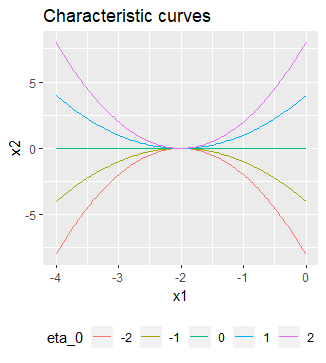
\includegraphics{ss1_p1a}
\caption{Characteristic curves $x_2 = \eta_0(x_1 + 2)^2$.}
\label{f1}
\end{figure}
Figure \ref{f2} shows the integral surface.
\begin{figure}
\centering
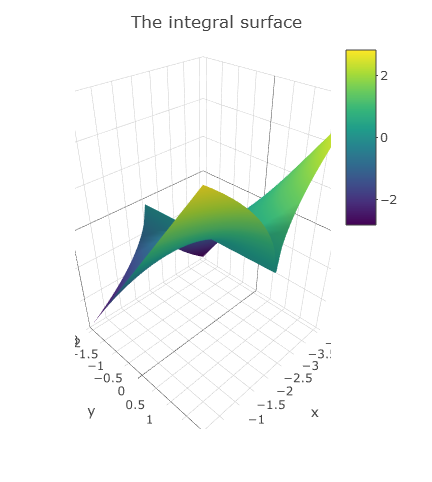
\includegraphics{ss1_p1b}
\caption{The integral surface $u(x) = \sqrt{x_2}(x_1 + 2)$.}
\label{f2}
\end{figure}

\item (Problem Set 1, Ex. 2) $x_1D^{e_1}u + x_2D^{e_2}u = 2u, x_1 > 0, x_2 > 0$ with initial 
conditions (a) $u = 1$ on the hyperbola $x_1x_2 = 1$ and (b) $u = 1$ on the circle $x_1^2 + x_2^2 = 
1$.

The parametric representation of the rectangular hyperbola $x_1x_2 = 1$ is $x_1 = \eta, x_2 = 
\eta^{-1}$. The parametric equation of the characteristic curves is
\begin{eqnarray}
D_\sigma x_1 &=& x_1 \label{s3e21} \\
D_\sigma x_2 &=& x_2 \label{s3e22} \\
D_\sigma u &=& 2u \label{s3e23},
\end{eqnarray}
subject to the initial conditions $x_1(\sigma = 0) = \eta_0, x_2(\sigma = 0) = \eta_0^{-1}$ and
$u(\sigma = 0) = 1$. Their solutions are
\begin{eqnarray}
x_1 &=& \eta_0 e^{\sigma} \label{s3e24} \\
x_2 &=& \eta_0^{-1} e^{\sigma} \label{s3e25} \\
u &=& e^{2\sigma} \label{s3e26}
\end{eqnarray}
The equation of characteristic curve is $x_2 = \eta_0^{-2}x_1$. It is a straight line passing
through the origin with slope $\eta_0^{-2}$. The first two of the above equations can be inverted 
to get
\begin{eqnarray}
e^\sigma &=& \sqrt{x_1x_2} \label{s3e27} \\
\eta_0 &=& \sqrt{\frac{x_1}{x_2}} \label{s3e28}
\end{eqnarray}
so that the solution of the problem is
\begin{equation}\label{s3e29}
u(x) = x_1x_2.
\end{equation}
Further, the Jacobian of transformation is
\[
\frac{\partial(x_1, x_2)}{\partial(\sigma, \eta_0)} = -\frac{2e^\sigma}{\eta_0} \ne 0
\]
so that the inversion is always possible.

The parametric representation of the circle $x_1^2 + x_2^2 = 1$ is $x_1 = \cos\eta$ and $x_2 = 
\sin\eta$. The parametric equations of the characteristic curves and $u$ are \eqref{s3e21}, 
\eqref{s3e22} and \eqref{s3e23} but now the initial conditions are $x_1(\sigma = 0) = \cos\eta_0$,
$x_2(\sigma = 0) = \sin\eta_0$ and $u(\sigma = 0) = 1$. Therefore, their solutions are
\begin{eqnarray}
x_1 &=& e^{\sigma}\cos\eta_0  \label{s3e30} \\
x_2 &=& e^{\sigma}\sin\eta_0 \label{s3e31} \\
u &=& e^{2\sigma} \label{s3e32}
\end{eqnarray}
The equation of the characteristic curve is $x_2 = x_1\tan\eta_0$. It is a straight line passing
through the origin with a slope $\tan\eta_0$. The first two of the above equations can be inverted 
to get
\begin{eqnarray}
e^\sigma &=& \sqrt{x_1^2 + x_2^2} \label{s3e33} \\
\eta_0 &=& \tan^{-1}\left(\frac{x_2}{x_1}\right) \label{s3e34}
\end{eqnarray}
Since $x_1 > 0, x_2 > 0$, these inversions are always possible and the solution of the problem is
\begin{equation}\label{s3e35}
u(x) = x_1^2 + x_2^2.
\end{equation}
Further, the Jacobian of transformation is
\[
\frac{\partial(x_1, x_2)}{\partial(\sigma, \eta_0)} = e^{2\sigma} \ne 0
\]
so that the inversion is always possible.

Now suppose that the initial curve was $x_2 = e^{x_1}$. Then we can parametrize it as $x_1 = \eta$
and $x_2 = e^\eta$. The initial conditions for the equations \eqref{s3e21}, \eqref{s3e22} and 
\eqref{s3e23} are $x_1(\sigma = 0) = \eta_0, x_2(\sigma = 0)$ and $u(\sigma = 0) = 1$ and hence
their solutions are
\begin{eqnarray}
x_1 &=& e^{\sigma}\eta_0  \label{s3e36} \\
x_2 &=& e^{\sigma + \eta_0} \label{s3e37} \\
u &=& e^{2\sigma}. \label{s3e38}
\end{eqnarray}
Once again, the characteristic curve is a straight line through the origin with equation 
\[
x_2 = \frac{e^{\eta_0}}{\eta_0}x_1.
\]
However, the Jacobian of transformation is
\[
\frac{\partial(x_1, x_2)}{\partial(\sigma, \eta_0)} = e^{2\sigma + \eta_0}(\eta_0 - 1) 
\]
so that the inversion is possible if $\eta_0 \ne 1$. 

\item (Problem Set 1, Ex. 3a) $x_1D^{e_1}u + x_2D^{e_2}u = ku, x \in \mathbb{R}, 0 < \alpha \le y$
with the initial condition $u(x, \alpha) = F(x)$, where $F$ is a smooth function. $k$ and $\alpha$ 
are constants.

The initial curve is a straight line parallel to the $x_1$ axis with parametric equation $x = \eta, y = 
\alpha$. The parametric equations of the characteristic curve and $u$ are
\begin{eqnarray}
D_\sigma x_1 &=& x_1 \label{s3e39} \\
D_\sigma x_2 &=& x_2 \label{s3e40} \\
D_\sigma u &=& ku \label{s3e41},
\end{eqnarray}
with initial conditions $x_1(\sigma = 0) = \eta_0, x_2(\sigma = 0) = \alpha, u(\sigma = 0) = 
F(\eta_0)$. The solutions of these equations are
\begin{eqnarray}
x_1 &=& \eta_0 e^\sigma \label{s3e42} \\
x_2 &=& \alpha e^\sigma \label{s3e43} \\
u &=& F(\eta_0)e^{k\sigma}. \label{s3e44}
\end{eqnarray}
The characteristics are straight lines with the equation 
\begin{equation}\label{s3e45}
x_2 = \frac{\alpha}{\eta_0}x_1
\end{equation}
Equations \eqref{s3e42} and \eqref{s3e43} can be inverted to get
\begin{eqnarray}
e^\sigma &=& \frac{x_2}{\alpha} \label{s3e46} \\
\eta_0 &=& \frac{\alpha x_1}{x_2} \label{s3e47}
\end{eqnarray}
Since the Jacobian of the transformation is $-\alpha e^{2\sigma}$, it is never zero and hence the
inversion of equations \eqref{s3e46} and \eqref{s3e47} is always possible. The solution of the problem
is then
\begin{equation}\label{s3e48}
u(x) = F\left(\frac{\alpha x_1}{x_2}\right)\left(\frac{x_2}{\alpha}\right)^k.
\end{equation}

\item (Problem Set 1, Ex. 3b) $(x_1 + 2)D^{e_1}u + 2x_2D^{e_2}u = \alpha u$ with initial condition 
$u(-1, x_2) = \sqrt{x_2}$. The initial curve is the line $x_1 = -1$. Its parametric form is $x_1 = -1,
x_2 = \eta$. The parametric equations of the characteristic curve along with the compatibility 
condition are
\begin{eqnarray}
D_\sigma x_1 &=& x_1 + 2 \label{s3e49} \\
D_\sigma x_2 &=& 2x_2 \label{s3e50} \\
D_\sigma u &=& \alpha u \label{s3e51}
\end{eqnarray}
with the initial conditions $x_1(\sigma = 0) = -1, x_2(\sigma = 0) = \eta, u(\sigma = 0) = 
\sqrt{\eta}$. Their solutions are
\begin{eqnarray}
x_1 &=& e^\sigma - 2 \label{s3e52} \\ 
x_2 &=& \eta_0 e^{2\sigma} \label{s3e53} \\
u &=& \sqrt{\eta_0}e^{\alpha\sigma} \label{s3e54}
\end{eqnarray}
The characteristic curve is $x_2 =\eta_0(x_1 + 2)^2$ and the Jacobian of transformation is $e^{2\sigma}
$ which is never zero so that the first two of the above equations can be inverted to get
\begin{eqnarray}
e^\sigma &=& x_1 + 2 \label{s3e55} \\
\eta_0 &=& \frac{x_2}{(x_1 + 2)^2}. \label{s3e56}
\end{eqnarray}
The solution of the problem is
\begin{equation}\label{s3e57}
u(x) = \sqrt{x_2}(x_1 + 2)^\alpha
\end{equation}

\item (Problem Set 1, Ex. 3c) $x_2D^{e_1}u - x_1D^{e_2}u = 0$ with $u(x_1, 0) = x_1^2$. The initial
curve is the line $x_2 = 0$ whose parametric form is $x_1 = \eta, x_2 = 0$. The parametric equations
of the characteristics along with the compatibility condition are
\begin{eqnarray}
D_\sigma x_1 &=& x_2 \label{s3e58} \\
D_\sigma x_2 &=& -x_1 \label{s3e59} \\
D_\sigma u &=& 0 \label{s3e60}
\end{eqnarray}
with initial conditions $x_1(\sigma = 0) = \eta_0, x_2(\sigma = 0) = 0, u(\sigma = 0) = 0$. 
Differentiating equation \eqref{s3e58} with respect to $\sigma$, $D_{\sigma\sigma} = -x_1$, whose
solution is $x_1 = a\cos\sigma + b\sin\sigma$. Substituting it in \eqref{s3e58} we immediately get
$x_2 = -a\sin\sigma + b\cos\sigma$. The initial conditions give $a = \eta$ and $b = 0$ so that
the solutions of the first two equations are
\begin{eqnarray}
x_1 &=& \eta\cos\sigma \label{s3e61} \\
x_2 &=& -\eta\sin\sigma \label{s3e62}
\end{eqnarray}
The solution of equation \eqref{s3e60} is $u(\sigma) = c$, which after using the initial conditions
gives $u(\sigma) = \eta^2$. Using equations \eqref{s3e61} and \eqref{s3e62} in the expression for $u$
we get the solution
\begin{equation}\label{s3e63}
u(x) = x_1^2 + x_2^2.
\end{equation}

\item (Problem Set 1, Ex. 3d) $x_1^2D^{e_1}u - x_2^2D^{e_2}u = 0$ with $u(1, x_2) = F(x_2)$. The 
initial curve is the line $x_1 = 1$ whose parametric form is $x_1 = 1, x_2 = \eta$. The parametric
equations of the characteristics along with the compatibility condition are
\begin{eqnarray}
D_\sigma x_1 &=& x_1^2 \label{s3e64} \\
D_\sigma x_2 &=& -x_2^2 \label{s3e65} \\
D_\sigma u &=& 0 \label{s3e66}
\end{eqnarray}
with initial conditions $x_1(\sigma = 0) = 1, x_2(\sigma = 0) = \eta, u(\sigma = 0) = F(x_2)$. The 
solution to the first two equations are
\begin{eqnarray*}
-\frac{1}{x_1} &=& \sigma + a \\
\frac{1}{x_2} &=& \sigma + b.
\end{eqnarray*}
Using the initial conditions, we get $a = -1$ and $b = \eta^{-1}$ so that
\begin{eqnarray}
1 -\frac{1}{x_1} &=& \sigma \label{s3e67} \\
\frac{1}{x_2} &=& \sigma + \frac{1}{\eta} \label{s3e68}.
\end{eqnarray}
The solution of \eqref{s3e66} is $u = c$. With the initial conditions $u(\sigma) = F(\eta)$. Using
equations \eqref{s3e67} and \eqref{s3e68} we get the solution
\begin{equation}\label{s3e69}
u(x) = F\left(\frac{x_1x_2}{x_1 + x_2 - x_1x_2}\right).
\end{equation} 

\item (Problem Set 1, Ex. 4) Find the characteritic curves of
\begin{enumerate}
\item $(x_1^2 - x_2^2 + 1)D^{e_1}u + 2x_1x_2D^{e_2}u = 0$. The equations of characteristics are
\[
\frac{dx_1}{x_1^2 - x_2^2 + 1} = \frac{dx_2}{2x_1x_2}.
\]
This is an exact differential of
\[
f(x_1, x_2) = x_1^2x_2 - \frac{x_2^3}{3} + x_2 = c,
\]
where $c$ is a constant. This is also the equation of characteristics.
\item $2x_1x_2D^{e_1}u - (x_1^2 + x_2^2)D^{e_2}u = 0$. The equations of characteristics are
\[
\frac{dx_1}{2x_1x_2} = -\frac{dx_2}{x_1^2 + x_2^2}.
\]
This is an exact differential of
\[
f(x_1, x_2) = x_1x_2^2 + \frac{x_1^3}{3} + x_2 = c,
\]
where $c$ is a constant. This is also the equation of characteristics.
\end{enumerate}
\end{enumerate}

\section{First Order Quasilinear PDE}\label{s4}
Continuing to work with the simple case of two independent variables, the general form of a 
quasilinear PDE is given by \eqref{s2e4}
\[
a_1(x_1, x_2, u)D^{e_1}u + a_2(x_1, x_2, u)D^{e_2}u = a_3(x_1, x_2, u).
\]
If we define $f = u(x_1, x_2) - x_3$ then the above equation can be written as
\begin{equation}\label{s4e1}
(a_1, a_2, a_3)\cdot Df = 0
\end{equation}
The gradient vector $Df$ is normal to the surface $f = 0$. Therefore, the vector $(a_1, a_2, a_3)$ is
tangent to it. The direction of $(a_1, a_2, a_3)$ at any point $(x_1, x_2, x_3)$ is called the 
\emph{Monge direction}. A surface $x_3 = u(x_1, x_2)$ is an integral surface if and only if at every
point on it, the tangent plane at the point contains the Monge direction. A space curve whose tangent
at every point coincides with the Monge direction is called the \emph{Monge curve}. Its parametric
equations are
\begin{eqnarray}
D_\sigma x_1 &=& a_1(x_1, x_2, u) \label{s4e2} \\
D_\sigma x_2 &=& a_2(x_1, x_2, u) \label{s4e3} \\
D_\sigma x_3 &=& a_3(x_1, x_2, u) \label{s4e4}
\end{eqnarray}
A solution to this system of ODEs is a $2$-parameter family of curves. (We can combine them to get
$D_{x_1}x_2 = a_2/a_1$ and $D_{x_1}x_3 = a_3/a_1$. Solving them gives one constant for each one of
them.) A particular solution of these equations will need two conditions at $\sigma = 0$ for each
one of $x_1, x_2, x_3$. They are provided by conditions of the form $x_1 = X_1(\eta_1, \eta_2), 
x_2 = X_2(\eta_1, \eta_2), x_3 = X_3(\eta_1, \eta_2)$, defining the `initial surface' of the problem.
The Monge curves, thus, are a $2$-parameter family of curves with parametric equations $x_1 = x_1(
\sigma, \eta_1, \eta_2), x_2 = x_2(\sigma, \eta_1, \eta_2), x_3 = x_3(\sigma, \eta_1, \eta_2)$.

The projection of the Monge curve on the $x_1x_2$ plane is called the characteristic curve of the
problem.

We argued that the Monge curves are a $2$-parameter family of curves. However, we can always fix
one of the parameters to a constant, say $0$, and consider them as a $1$-parameter family of
curves. We will show that the $1$-parameter sub-family of Monge curves is equally good to find 
solutions of a quasi-linear PDE.
\begin{thm}\label{s4t1}
Every surface generated by a $1$-parameter sub-family of Monge curves is an integral surface.
\end{thm}
\begin{proof}
Consider a surface generated by a $1$-parameter sub-family of Monge curves obtained by setting the 
second parameter to a constant, say $\eta_0$. At every point on this surface the Monge direction 
coincides with the tangent to the surface. Therefore, the tangent plane at every point has the
Monge vector, making it an integral surface.
\end{proof}

The converse of the above theorem is also true.
\begin{thm}\label{s4t2}
Every integral surface can be considered to be generated by a $1$-parameter sub-family of Monge
curves.
\end{thm}
\begin{proof}
Let $x_3 = u(x_1, x_2)$ be an integral surface of the quasi-linear PDE
\begin{equation}\label{s4e5}
a_1(x_1, x_2, u)D^{e_1}u + a_2(x_1, x_2, u)D^{e_2}u = a_3(x_1, x_2, u)
\end{equation}
and let $x_1 = X_1(\eta), x_2 = X_2(\eta)$ and
$x_3 = u(X_1(\eta), X_2(\eta))$ be the space curve on it. Further, let us assume that the curve does 
not coincide with a Monge curve. Consider a solution of the system of equations
\begin{eqnarray*}
D_\sigma x_1 &=& a_1(x_1, x_2, x_3(x_1, x_2)) \label{s4e6} \\
D_\sigma x_2 &=& a_2(x_1, x_2, x_3(x_1, x_2)) \label{s4e7}
\end{eqnarray*}
with initial conditions $x_1(\sigma = 0) = X_1(\eta), x_2(\sigma = 0) = X_2(\eta)$. Since $x_3 = 
u(x_1, x_2)$ on the surface,
\begin{equation}\label{s4e8}
D_\sigma x_3 = D_\sigma x_1D^{e_1}u + D_\sigma x_1D^{e_1}u.
\end{equation}
Using the first three equations in the fourth one we get
\begin{equation}\label{s4e9}
D_\sigma x_3 = a_3(x_1, x_2, u).
\end{equation}
Equations \eqref{s4e6}, \eqref{s4e7} and \eqref{s4e9} tell that the curve $(x_1(\sigma, \eta), 
x_2(\sigma, \eta), x_3(\sigma, \eta))$ passing through a point $X_1(\eta), X_2(\eta), X_3(\eta)$ on the 
integral surface is a Monge curve. Thus, any integral surface can be generated by a $1$-parameter
family of Monge curves.
\end{proof}

The following theorem suggests a way to solve the Cauchy problem for a first-order quasi-linear PDE.
\begin{thm}\label{s4t3}
Let $X_i: [0, 1] \rightarrow \mathbb{R}$, $i = 1, 2, 3$, be continuously differentiable functions. 
Let $a_1, a_2, a_3: U_2 \rightarrow \mathbb{R}$, where $U_2 \subset \mathbb{R}^3$, have
continuous first order partial derivatives throughout $U_2$. Let the initial curve 
\[
\Gamma = \{(X_1(\eta), X_2(\eta), X_3(\eta): \eta \in [0, 1]\},
\]
be entirely in $U_2$ such that
\[
D_\eta X_2(\eta) a_1(X_1(\eta), X_2(\eta), X_3(\eta)) \ne 
D_\eta X_1(\eta) a_2(X_1(\eta), X_2(\eta), X_3(\eta)).
\]
Then there exists a solution $u(x_1, x_2)$ of the quasi-linear PDE
\[
a_1(x_1, x_2, u)D^{e_1}u + a_2(x_1, x_2, u)D^{e_2}u = a_3(x_1, x_2, u)
\]
in the neighborhood of the datum curve 
\[
\gamma = \{(X_1(\eta), X_2(\eta): \eta \in [0, 1]\},
\]
such that $u(\eta) = u(X_1(\eta), X_2(\eta))$.
\end{thm}
\begin{proof}
Since $a_1, a_2, a_3: U_2 \rightarrow \mathbb{R}$, where $U_2 \subset \mathbb{R}^3$, have
continuous first order partial derivatives throughout $U_2$, the system of equations
\begin{eqnarray*}
D_\sigma x_1 &=& a_1 \\
D_\sigma x_2 &=& a_2 \\
D_\sigma x_3 &=& a_3,
\end{eqnarray*}
where we have used $x_3 = u$, has a unique, continuously differentiable solution satisfying the
initial conditions
\begin{eqnarray*}
x_1(0, \eta) &=& X_1(\eta) \\
x_2(0, \eta) &=& X_2(\eta) \\
x_3(0, \eta) &=& X_3(\eta).
\end{eqnarray*}
Therefore, the functions $X_1, X_2, X_3$ too are continuously differentiable functions of $\eta$.
We assumed that the Jacobian
\[
\frac{\partial(x_1, x_2)}{\partial(\sigma, \eta)} = \pd{x_1}{\sigma}\pd{x_2}{\eta} - 
\pd{x_1}{\eta}\pd{x_2}{\sigma} = a_1\pd{x_2}{\eta} - a_2\pd{x_1}{\eta} \ne 0.
\]
Therefore, in the neighborhood of $\sigma = 0$, we can invert the relations $x_1 = x_1(\sigma, \eta)$
and $x_2 = x_2(\sigma, \eta)$ to get $\sigma = \sigma(x_1, x_2)$ and $\eta = \eta(x_1, x_2)$ and
substitute them in $x_3(\sigma, \eta)$ to get the solution in the form $x_3 = u(x_1, x_2)$. Further,
at any point on the datum curve $u(X_1(\eta), X_2(\eta)) = u(0, \eta) = x_3(0, \eta) = X_3(\eta)$
so that the initial condition on $D_\sigma x_2 = a_3$ is also satisfied.

We will now prove that the solution $u$ is unique. Let there be two integral surfaces $S_1$ and $S_2$
passing through the initial curve $\Gamma$. Let $(X_1(\eta_0), X_2(\eta_0), X_3(\eta_0)$ be a point 
common to both surfaces. Then the Monge curve through it is also common to both surfaces. Thus, both
surfaces are generated by the same family of Monge curves, which means that the two surfaces are 
identical.
\end{proof}

\section{Examples of Quasi-linear PDE}\label{s5}
\begin{enumerate}
\item (Example 1.10.2 of \cite{ta}) $uD^{e_1}u + D^{e_2}u = 1$ with the initial data $x_0 = s, y_0 = s,
u_0 = s/2$ for $s \in [0, 1]$. The parametric equations of the characteristics are
\begin{eqnarray}
D_\sigma x_1 &=& x_3 \label{s5e1} \\
D_\sigma x_2 &=& 1 \label{s5e2} \\
D_\sigma x_3 &=& 1 \label{s5e3}.
\end{eqnarray}
From equations \eqref{s5e3} and \eqref{s5e1},
\begin{equation}\label{s5e4}
D^2_\sigma x_1 = 1
\end{equation}
Therefore,
\begin{eqnarray}
x_1 &=& \frac{\sigma^2}{2} + c_1\sigma + c_2 \label{s5e5} \\
x_2 &=& \sigma + c_3 \label{s5e6} \\
x_3 &=& \sigma + c_4. \label{s5e7}
\end{eqnarray}
The initial conditions are $x_1(0, \eta) = s, x_2(0, \eta) = s, x_3(0, \eta) = s/2$. Therefore, the
solutions are
\begin{eqnarray}
x_1 &=& \frac{\sigma^2}{2} + c_1\sigma + s \label{s5e8} \\
x_2 &=& \sigma + s \label{s5e9} \\
x_3 &=& \sigma + \frac{s}{2}. \label{s5e10}
\end{eqnarray}
From equations \eqref{s5e1}, \eqref{s5e8} and \eqref{s5e10} we conclude that $c_1 = s/2$ so that
\begin{equation}\label{s5e11}
x_1 = \frac{\sigma^2}{2} + \frac{\sigma}{2}s + s
\end{equation}
We obtained the solution $u = x_3$ in terms of $s$ and $\sigma$. We need it in terms of $x_1, x_2$.
From equations \eqref{s5e11} and \eqref{s5e9},
\[
x_1 - x_2 = \frac{\sigma^2}{2} + \frac{\sigma}{2}s - \sigma = \frac{\sigma}{2}(\sigma + s) - \sigma
= \frac{\sigma}{2}x_2 - \sigma = \sigma\left(\frac{x_2}{2} - 1\right),
\]
so that
\begin{equation}\label{s5e12}
\sigma = \frac{x_1 - x_2}{x_2/2 - 1}.
\end{equation}
Using \eqref{s5e9}, we get
\begin{equation}\label{s5e13}
s = \frac{x_2^2/2 - x_1}{x_2/2 - 1}
\end{equation}
so that the solution of the problem is 
\begin{equation}\label{s5e14}
x_3 = u(x_1, x_2) = \frac{x_1 - x_2}{x_2/2 - 1} + \frac{1}{2}\frac{x_2^2/2 - x_1}{x_2/2 - 1} = 
\frac{2x_1 - 4x_2 + x_2^2}{2(x_2 - 2)}.
\end{equation}

\item (Example 2.3 of \cite{pprr}) $uD^{e_1}u + D^{e_2}u = 0$ with intial data (a) $u(x_1, 0) = x_1$
for $x_1 \in [0, 1]$ and (b) $u(x_1, 0) = 1/2$ for $x_1 \in [0, 1]$.

The parametric form of the data are (a) $\{x_1 = \eta, x_2 = 0, u (=x_3) = \eta\}$ and (b) $\{x_1 = 
\eta, x_2 = 0, x_3 = 1/2\}$.

The parametric equations of the Monge curves are
\begin{eqnarray*}
D_\sigma x_1 &=& u \\
D_\sigma x_2 &=& 1 \\
D_\sigma x_3 &=& 0
\end{eqnarray*}
Their solutions for the two data sets are
\begin{eqnarray*}
x_1 &=& \eta\sigma + \eta \\
x_2 &=& \sigma \\
x_3 &=& \eta
\end{eqnarray*}
and
\begin{eqnarray*}
x_1 &=& \frac{\sigma}{2}\sigma + \eta\\
x_2 &=& \sigma \\
x_3 &=& \frac{1}{2}
\end{eqnarray*}
respectively so that the characteristic curves are the lines $x_1 = \eta(x_2 + 1)$ and $x_1 = 
x_2/2 + \eta$. They are shown in figure \ref{f3}.
\begin{figure}
\centering
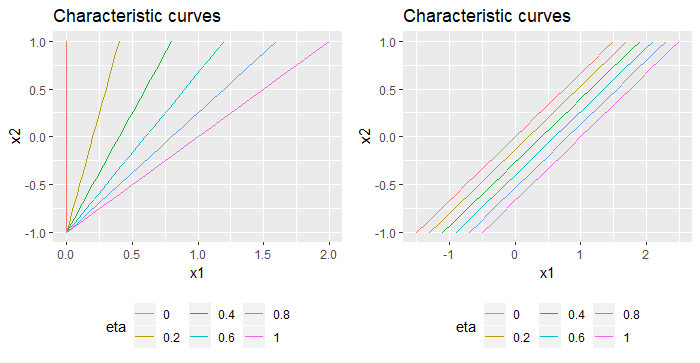
\includegraphics[scale=0.75]{cnf1}
\caption{Characteristic curves for the initial data.}
\label{f3}
\end{figure}

The characteristics $x_1 = \eta(x_2 + 1)$ all meet at the point $(0, -1)$. It happens because of the
form of the solution
\[
u = x_3 = \eta = \frac{x_1}{x_2 + 1}.
\]
Clearly, $u(x_1, x_2)$ has a singularity at $x_2 = -1$.

\item (Problem Set 1. Ex. 5b) $uD^{e_1}u + D^{e_2}u = 1$, $u(x, x) = x/2$ for $x \in [0, 1]$. The
parametric equations of the Monge curves are
\begin{eqnarray}
D_\sigma x_1 &=& u \label{s5e15} \\
D_\sigma x_2 &=& 1 \label{s5e16} \\
D_\sigma x_3 &=& 1 \label{s5e17}.
\end{eqnarray}
The general solution of \eqref{s5e17} is 
\begin{equation}\label{s5e18}
x_3 = \sigma + c_1
\end{equation}
so that the general solution of \eqref{s5e15} becomes 
\begin{equation}\label{s5e19}
x_1 = \frac{\sigma^2}{2} + c_1\sigma + c_2.
\end{equation}
Finally, the general solution of \eqref{s5e16} is
\begin{equation}\label{s5e20}
x_2 = \sigma + c_3.
\end{equation}
The initial data is $x_1(\sigma = 0, \eta) = \eta, x_2(\sigma = 0, \eta) = \eta \rightarrow 
x_3(\sigma = 0, \eta) = \eta/2$. Therefore $c_1 = \eta/2$, $c_2 = \eta$ and $c_3 = \eta$. Therefore
\begin{eqnarray}
x_1 &=& \frac{\sigma^2}{2} + \frac{\eta}{2}\sigma + \eta \label{s5e21} \\
x_2 &=& \sigma + \eta \label{s5e22} \\
x_3 &=& \sigma + \frac{\eta}{2} \label{s5e23}
\end{eqnarray}
The transversality condition is
\[
\frac{\partial(x_1, x_2)}{\partial(\sigma, \eta)} = \pd{x_1}{\sigma}\pd{x_2}{\eta} - 
\pd{x_1}{\eta}\pd{x_2}{\sigma} = \left(\sigma + \frac{\eta}{2}\right) - 
\left(\frac{\sigma}{2} + 1\right) = \frac{\sigma + \eta}{2} - 1
\]
Thus,
\[
\frac{\partial(x_1, x_2)}{\partial(\sigma, \eta)} \ne 1
\]
as long as $\sigma + \eta \ne 2$. This is definitely true for $x_1, x_2 \in [0, 1]$. Inverting
equations \eqref{s5e21} and \eqref{s5e22} we get
\begin{eqnarray}
\sigma &=& \frac{2(x_2 - x_1)}{2 - x_1} \label{s5e24} \\
\eta &=& \frac{x_2(2 - x_1)}{2 - x_1} \label{s5e25}
\end{eqnarray}
Using \eqref{s5e23}, \eqref{s5e24} and \eqref{s5e25} we get
\begin{equation}\label{s5e26}
u(x_1, x_2) = \frac{2(x_2 - x_1)}{2 - x_1} + \frac{1}{2}\frac{x_2(2 - x_1)}{2 - x_1}
\end{equation}

\item (Problem Set 1, Ex. 6) $uD^{e_1}u + D^{e_2}u = 0$ with several different initial conditions.
The parametric equations of the Monge curve are
\begin{eqnarray}
D_\sigma x_1 &=& x_3 \label{s5e27} \\
D_\sigma x_2 &=& 1 \label{s5e28} \\
D_\sigma x_3 &=& 0 \label{s5e29}
\end{eqnarray}
their general solution of which is
\begin{eqnarray}
x_1 &=& c_1\sigma + c_2 \label{s5e30} \\
x_2 &=& \sigma + c_3 \label{s5e31} \\
x_3 &=& c_1 \label{s5e32}
\end{eqnarray}
Let us now examine the various initial conditions.
\begin{enumerate}
\item \begin{equation}\label{s5e33}
u(x, 0) = \begin{cases}
0 \text{ if } x < 0 \\
1 \text{ if } x \ge 0
\end{cases}
\end{equation}
The parametric equations of the Monge curves are
\begin{equation}\label{s5e34}
x_1 = \begin{cases}
\eta \text{ if } x_1 < 0 \\
\sigma + \eta \text{ if } x_1 \ge 0
\end{cases}
\end{equation}
\begin{equation}\label{s5e35}
x_2 = \sigma
\end{equation}
We can combine equations \eqref{s5e34} and \eqref{s5e35} to get
\begin{equation}\label{s5e36}
x_1 = \begin{cases}
\eta \text{ if } x_1 < 0 \\
x_2 + \eta \text{ if } x_1 \ge 0
\end{cases}
\end{equation}
Thus, the characteristic curve is the negative $x_1$ axis and the parallel lines $x_2 = x_1 - \eta$
with $x_1 \ge 0$ for all $\eta$.

\item \begin{equation}\label{s5e37}
u(x, 0) = \begin{cases}
1 \text{ if } x < 0 \\
0 \text{ if } x \ge 0
\end{cases}
\end{equation}
The parametric equations of the Monge curves are
\begin{equation}\label{s5e38}
x_1 = \begin{cases}
\sigma + \eta \text{ if } x_1 < 0 \\
\eta \text{ if } x_1 \ge 0
\end{cases}
\end{equation}
\begin{equation}\label{s5e39}
x_2 = \sigma
\end{equation}
We can combine equations \eqref{s5e34} and \eqref{s5e35} to get
\begin{equation}\label{s5e40}
x_1 = \begin{cases}
\sigma + \eta \text{ if } x_1 < 0 \\
\eta \text{ if } x_1 \ge 0
\end{cases}
\end{equation}
Thus, the characteristic curve is the positive $x_1$ axis and the parallel lines $x_2 = x_1 - \eta$
with $x_1 \ge 0$ for all $\eta$.

\item \begin{equation}\label{s5e41}
u(x, 0) = \begin{cases}
0 \text{ if } x < 0 \\
1 \text{ if } x \ge 1
\end{cases}
\end{equation}
and $u(x, 0)$ is smooth and increasing in $[0, 1]$. Let us denote it by $\phi(x)$. Thus,
\begin{equation}\label{s5e42}
u(x, 0) = \begin{cases}
0 \text{ if } x < 0 \\
\phi(x) \text{ if } x \in [0, 1] \\
1 \text{ if } x \ge 1
\end{cases}
\end{equation}
for a smooth and increasing $\phi$. Thus the parametric equations of the Monge curves are $x_2 = 
\sigma$ and 
\begin{equation}\label{s5e43}
x_1 = \begin{cases}
\eta \text{ if } x_1 < 0 \\
\phi(\eta) \text{ if } x_1 \in [0, 1] \\
\sigma + \eta \text{ if } x_1 \ge 1
\end{cases}
\end{equation}
or
\begin{equation}\label{s5e44}
x_1 = \begin{cases}
\eta \text{ if } x_1 < 0 \\
\phi(\eta) \text{ if } x_1 \in [0, 1] \\
x_2 + \eta \text{ if } x_1 \ge 1
\end{cases}
\end{equation}
The characteristic curves is the negative $x_1$ axis, the function $\phi(\eta)$ for $x_1 \in [0, 1]$
and the lines $x_2 = x_1 - \eta$ for $x_1 > 1$.
\end{enumerate}
\end{enumerate}

\section{On envelopes of surfaces}\label{s6}\cite{fj}
Consider a one-parameter family of surfaces $S_\lambda$ defined by
\begin{equation}\label{s6e1}
x_3 = G(x_1, x_2, \lambda),
\end{equation}
where $\lambda$ is the parameter. Differentiating both sides with respect to $\lambda$, we get
\begin{equation}\label{s6e2}
0 = \pd{G}{\lambda}(x_1,x_2,\lambda).
\end{equation}
In principle, we can solve this equation to get $\lambda = g(x, y)$ so that the equation of the 
surface can be written as 
\begin{equation}\label{s6e3}
x_3 = G(x_1, x_2, g(x_1, x_2)).
\end{equation}
Equation \eqref{s6e3} defines the envelope $E$ of all one-parameter surfaces defined by \eqref{s6e1}.
It touches all surfaces $S_\lambda$ alonga curve $\gamma_\lambda$. Consider a point $(X_1, X_2, X_3)$
on one such curve $\gamma_\lambda$. Since it lies on a curve with parameter $\lambda$, we naturally
have $g(X_1, X_2) = \lambda$. The direction numbers of the normal to the envelope $E$ are
\[
D(G(x_1, x_2, g(x_1, x_2)) - x_3) = 
\left(\pd{G}{x_1} + \td{G}{\lambda}\pd{g}{x_1}, \pd{G}{x_2} + \td{G}{\lambda}\pd{g}{x_2}, -1\right)
\]
Using \eqref{s6e2}, we have
\[
D(G(x_1, x_2, g(x_1, x_2)) - x_3) = \left(\pd{G}{x_1}, \pd{G}{x_2}, -1\right)
\]
Naturally, these are same as the direction numbers of a normal to $S_\lambda$ given by \eqref{s6e1}. 
In the future, we will find it advantageous to use the differential forms of equations \eqref{s6e1}
\begin{equation}\label{s6e4}
dx_3 = D^{e_1}Gdx_1 + D^{e_2}Gdx_2
\end{equation}
and
\[
0 = \frac{\partial^2 G}{\partial x_1 \partial\lambda}dx_1 +
\frac{\partial^2 G}{\partial x_2 \partial\lambda}dx_2 + 
\frac{\partial^2 G}{\partial\lambda^2}d\lambda.
\]
Now on a curve $\gamma_\lambda$, $\lambda$ is fixed so that
\begin{equation}\label{s6e5}
0 = \frac{\partial^2 G}{\partial x_1 \partial\lambda}dx_1 + 
\frac{\partial^2 G}{\partial x_2 \partial\lambda}dx_2.
\end{equation}

\section{First order nonlinear PDE}\label{s7}
The general form of a first order nonlinear PDE is given by \eqref{s2e1}
\begin{equation}\label{s7e1}
F(x_1, x_2, u, p, q) = 0
\end{equation}
where $F:U^2 \times \mathbb{R} \times U^2 \rightarrow \mathbb{R}$, $D^{e_1}u = p$ and  
$D^{e_2}u = q$. If $f = u(x_1, x_2) - x_3$ then $Df = (p, q, -1)$ is a normal to the integral surface.
A plane normal to $Df$ will be tangent to the integral surface. Its general equation is
\begin{equation}\label{s7e2}
p(x_1 - x_1^0) + q(x_2 - x_2^0) - 1(x_3 - x_3^0) = 0,
\end{equation}
where $(x_1^0, x_2^0, x_3^0)$ is an arbitrary, but fixed, point on it. As yet, we do not know the 
solution $x_3 = u(x_1, x_2)$. Therefore, we do not know $p$ and $q$. Yet, we know that they are not
both arbitrary because they are related by equation \eqref{s7e1}. If we fix one of them, say $p$,
then \eqref{s7e1} gives the other and therefore equation \eqref{s7e2} is a one-parameter family of
planes passing through the point $(x_1^0, x_2^0, x_3^0)$. An envelope of this family of planes is
a cone, called the \emph{Monge cone}. There is a Monge cone on every point of the integral surface.
Equation \eqref{s7e1} can as well be interpreted as defining a field of Monge cones. The integral 
surface of the problem is tangent to all cones. Therefore, only one plane in the envelope of a given
Monge cone is tangential to the integral surface. Its generator defines the \emph{Monge direction} at 
that point.

For a fixed $p$ (and therefore also a fixed $q$ by virtue of \eqref{s7e1}), differentiating \
\eqref{s7e2} gives
\begin{equation}\label{s7e3}
pdx_1 + qdx_2 = dx_3.
\end{equation}
We can also differentiate \eqref{s7e2} with respect to the `parameter' $p$ to get the relation
\[
(x_1 - x_1^0) + \td{q}{p}(x_2 - x_2^0) = 0.
\]
If we differentiate it once more and retain only the first order terms we get
\begin{equation}\label{s7e4}
dx_1 + \td{q}{p}dx_2 = 0
\end{equation}
which can be written as 
\begin{equation}\label{s7e5}
\td{q}{p} = -\frac{dx_1}{dx_2}.
\end{equation}
From equation \eqref{s7e1} we get
\[
F_{p}dp + F_{q}dq = 0
\]
which is same as
\begin{equation}\label{s7e6}
\td{q}{p} = -\frac{F_{p}}{F_{q}}.
\end{equation}
From equations \eqref{s7e5} and \eqref{s7e6} we get
\begin{equation}\label{s7e7}
\frac{dx_1}{F_{p}} = \frac{dx_2}{F_{q}}.
\end{equation}
If $\sigma$ is a parameter then the previous equation also means
\begin{eqnarray}
\td{x_1}{\sigma} &=& F_{p} \label{s7e8} \\
\td{x_2}{\sigma} &=& F_{q} \label{s7e9}
\end{eqnarray}
so that if we also differentiate equation \eqref{s7e3} with respect to $\sigma$ we get
\begin{equation}\label{s7e10}
\td{x_3}{\sigma} = p\td{x_1}{\sigma} + q\td{x_2}{\sigma}.
\end{equation}
Equation \eqref{s7e10} is also called the \emph{strip condition}. In fact, we can combine equations 
\eqref{s7e8}, \eqref{s7e9} and \eqref{s7e10} to get
\begin{equation}\label{s7e11}
\frac{dx_1}{F_{p}} = \frac{dx_2}{F_{q}} = \frac{dx_3}{pF_{p} + qF_{q}}
\end{equation}
This is the parametric equation of the Monge curves. 

For a quasi-linear equation $F = a_1(x_1, x_2, u)p + a_2(x_1, x_2, u)q - a_3(x_1, x_2, u)$ so that 
equation \eqref{s7e11} gives
\[
\frac{dx_1}{a_1} = \frac{dx_2}{a_2} = \frac{dx_3}{pa_1 + qa_2}.
\]
Since $pa_1 + qa_2 = a_2$, we get
\[
\frac{dx_1}{a_1} = \frac{dx_2}{a_2} = \frac{dx_3}{a_3}
\]
which is just another form of equations the parametric equations \eqref{s4e2} to \eqref{s4e4} of its
Monge curve. 

Coming back to equation \eqref{s7e11}, we have derived three equations for three unknowns $x_1, x_2,
x_3$ as functions of $\sigma$. We have two more unknowns $p$ and $q$. We need a differential equation
for each one of them in terms of the parameter $\sigma$. To get them we begin with the definition 
$p = D^{e_1}u$ so that
\begin{equation}\label{s7e12}
\td{p}{\sigma} = \frac{\partial^2 u}{\partial x_1^2}\td{x_1}{\sigma} + 
\frac{\partial^2 u}{\partial x_1\partial x_2}\td{x_2}{\sigma} 
\end{equation}
Using \eqref{s7e11}, we get
\begin{equation}\label{s7e13}
\td{p}{\sigma} = \pd{p}{x_1}F_{p} + \pd{p}{x_2}F_{q}
\end{equation}
Since $F(x_1, x_2, u, p, q) = 0$, we also have
\begin{equation}\label{s7e14}
\pd{F}{x_1} + \pd{F}{u}\pd{u}{x_1} + F_{p}\pd{p}{x_1} + F_{q}\pd{q}{x_1} = 0
\end{equation}
From equations \eqref{s7e13} and \eqref{s7e14} we get the parametric equation of $p$ 
\begin{equation}\label{s7e15}
D_\sigma p = -F_{x_1} - F_up.
\end{equation}
Similarly, from equation
\begin{equation}\label{s7e16}
\td{q}{\sigma} = \frac{\partial^2 u}{\partial x_1\partial x_2}\td{x_1}{\sigma} +
\frac{\partial^2 u}{\partial x_2^2}\td{x_2}{\sigma} = \pd{q}{x_1}F_{p} + \pd{q}{x_2}F_{q}
\end{equation}
and
\begin{equation}\label{s7e17}
\pd{F}{x_2} + \pd{F}{u}\pd{u}{x_2} + F_{p}\pd{q}{x_1} + F_{q}\pd{q}{x_2} = 0
\end{equation}
we get the parametric equation for $q$ as
\begin{equation}\label{s7e18}
D_\sigma q = -F_{x_2} - F_uq.
\end{equation}
Note that
\[
\pd{q}{x_1} = \pd{q}{x_2}.
\]
makes equations \eqref{s7e14} and \eqref{s7e17} identical. The equations of the Monge curves are 
\begin{equation}\label{s7e19}
\frac{dx_1}{F_{p}} = \frac{dx_2}{F_{q}} = \frac{dx_3}{pF_{p} + qF_{q}} = 
\frac{dp}{-F_{x_1} - F_{u}p} = \frac{dq}{-F_{x_2} - F_{u}q}
\end{equation}
Using these equations it is easy to conclude that
\begin{equation}\label{s7e20}
D_\sigma F = 0
\end{equation}
or that $F$ is constant along a Monge curve. Equation \eqref{s7e19} is a set of five ordinary 
differential equations. We need five initial conditions to solve them. Three are given by the initial
data. The initial values of $p$ and $q$ are obtained as follows. Let $p(\sigma = 0) = p_0$ and 
$q(\sigma = 0) = q_0$. Then the following equations are true
\begin{eqnarray}
F(x_1^0, x_2^0, u, p, q) &=& 0 \label{s7e21} \\
\td{x_3}{\sigma} = p_0\td{x_1}{\sigma} + q_0\td{x_2}{\sigma}. \label{s7e22} 
\end{eqnarray}
The second equation is just the strip condition \eqref{s7e10} at $\sigma = 0$.

\section{Examples of nonlinear PDE}\label{s8}
\begin{enumerate}
\item (Problem Set 1, Ex. 7) $q = p^3$ with the initial condition $u = 2x_1^{3/2}$ in the $x_1$ axis. 
Let us first get the initial data to solve the system of equations \eqref{s7e19}. Let it be $(x_1^0,
x_2^0, x_3^0 = u_0, p_0, q_0)$. The parameteric equation of the initial curve is $x_1 = \eta, x_2 = 0,
x_3 = 2\eta^{3/2}$. $p_0$ and $q_0$ can be chosen from the conditions
\begin{eqnarray}
q_0 &=& p_0^{3} \label{s8e1} \\
\td{x_3}{\eta} &=& p_0\td{x_1}{\eta} + q_0\td{x_2}{\eta} \label{s8e2}
\end{eqnarray}
The second equation reduces to
\[
3\eta^{1/2} = p_0 \cdot 1
\]
Using this equation in \eqref{s8e1} we get
\begin{eqnarray}
p_0 &=& 3\eta^{1/2} \label{s8e3} \\
q_0 &=& 3\eta^{3/2} \label{s8e4}
\end{eqnarray}
If we write the PDE as $F = p^3 - q = 0$ so that the equations of the characteristic strip are
\[
\frac{dx_1}{3p^2} = \frac{dx_2}{-1} = \frac{dx_3}{3p^3 - q} = \frac{dp}{} = \frac{dq}{}
\]
The system of ODE is
\begin{eqnarray}
D_\sigma x_1 &=& 3p^2 \label{s8e5} \\
D_\sigma x_2 &=& -1 \label{s8e6} \\
D_\sigma x_3 &=& 3p^3 - q \label{s8e7} \\
D_\sigma p &=& 0 \label{s8e8} \\
D_\sigma q &=& 0. \label{s8e9}
\end{eqnarray}
subject to the initial conditions $x_1(\sigma = 0) = \eta, x_2(\sigma = 0) = 0, x_3(\sigma = 0) =
 2\eta^{3/2}, p_0 = 3\eta^{1/2}, q_0 = 27\eta^{3/2}$.
 
The solutions of the last two equations are $p = p_0= 3\eta^{1/2}, q = q_0 = 27\eta^{3/2}$. The
solutions of first two equations are $x_1 = 3p_0^2\sigma + c_1$ and $x_2 = -\sigma + c_2$. Since the
initial data is on the $x_1$ axis, $x_1 = \eta$ and $x_2 = 0$ when $\sigma = 0$ so that we have
\begin{eqnarray}
x_1 &=& 27\eta\sigma + \eta \label{s8e10} \\
x_2 &=& -\sigma. \label{s8e11}
\end{eqnarray}
These equations can be inverted to get
\begin{eqnarray}
\sigma &=& -x_2 \label{s8e12} \\
\eta &=& \frac{x_1}{1 - 27 x_2} \label{s8e13}
\end{eqnarray}
The solution of \eqref{s8e7} subject to the initial condition $x_3(\sigma = 0) = 2\eta^{3/2}$ is
\begin{equation}\label{s8e14}
u = x_3 = 78\eta^{3/2}\sigma + 2\eta^{3/2} = 2\eta^{3/2}(27\sigma + 1).
\end{equation}
From equations \eqref{s8e13} and \eqref{s8e14} we get the solution
\begin{equation}\label{s8e15}
u(x_1, x_2) = \frac{2x_1^{3/2}}{(1 - 27x_2)^{1/2}}.
\end{equation}
It is easy to verify that
\begin{eqnarray*}
p &=& \frac{3x_1^{1/2}}{(1 - 27x_2)^{1/2}} \\
q &=& \frac{27x_1^{3/2}}{(1 - 27x_2)^{3/2}}
\end{eqnarray*}
so that $p^3 = q$.

\item (Problem Set 1, Ex. 8) $x_1p^2 + x_2q = u$ passing through the line $x_2 = 1$, $x_1 + x_3 = 0$.
Let $(x_1^0, x_2^0, x_3^0, p_0, q_0)$ be the initial data for the system of equations \eqref{s7e19}.
The parametric equations of the initial curve are $x_2 = 1, x_1 = \eta, x_3 = -\eta$. The initial
values of the first derivatives can be obtained from the equations
\begin{eqnarray*}
\eta p_0^2 + 1\cdot q_0 &=& -\eta \\
\td{x_3}{\eta} &=& p_0\td{x_1}{\eta} + q_0\td{x_2}{\eta}
\end{eqnarray*}
The second equation reduces to
\[
-1 = p_0\cdot 1 + q_0\cdot 0.
\]
From these equations we get
\begin{eqnarray}
p_0 &=& -1 \label{s8e16} \\
q_0 &=& -2\eta. \label{s8e17}
\end{eqnarray}

If we write the PDE as $F = x_1p^2 + x_2q - u = 0$ then the system of ODEs is
\begin{eqnarray}
D_\sigma x_1 &=& 2px_1 \label{s8e18} \\
D_\sigma x_2 &=& x_2 \label{s8e19} \\
D_\sigma x_3 &=& 2p^2x_1 + qx_2 \label{s8e20} \\
D_\sigma p &=& -p^2 + p \label{s8e21} \\
D_\sigma q &=& -q + q = 0 \label{s8e22}
\end{eqnarray}
The solution of the last equation is 
\begin{equation}\label{s8e23}
q(\sigma) = -2\eta.
\end{equation}
The solution of equation \eqref{s8e21} is
\begin{equation}\label{s8e24}
p(\sigma) = \frac{e^\sigma}{e^\sigma - 2}.
\end{equation}
Substituting it in \eqref{s8e18} we get
\begin{equation}\label{s8e25}
x_1(\sigma) = \eta(e^\sigma - 2)^2.
\end{equation}
The solution of \eqref{s8e19} is 
\begin{equation}\label{s8e26}
x_2(\sigma) = e^\sigma.
\end{equation}
Using \eqref{s8e23}, \eqref{s8e24},
\eqref{s8e25} in equation \eqref{s8e20} we get
\[
D_\sigma x_3 = 2\eta e^{2\sigma} - 2\eta e^\sigma
\]
so that
\[
x_3(\sigma) = \eta e^{2\sigma} - 2\eta e^\sigma + c,
\]
where $c$ is a constant of integration. Since $x_3(\sigma = 0) = -\eta$, we have
\begin{equation}\label{s8e27}
x_3(\sigma) = \eta e^{2\sigma} - 2\eta e^\sigma.
\end{equation}
Inverting \eqref{s8e24} and \eqref{s8e25}, we get
\begin{eqnarray}
e^\sigma &=& x_2 \label{s8e28} \\
\eta &=& \frac{x_1}{(x_2 - 2)^2} \label{s8e29}.
\end{eqnarray}
Substituting \eqref{s8e27} and \eqref{s8e28} in \eqref{s8e26} we get
\begin{equation}\label{s8e30}
u(x_1, x_2) = \frac{x_1x_2}{x_2 - 2}.
\end{equation}
We can readily verify that
\begin{eqnarray*}
p &=& \frac{x_2}{x_2 - 2} \\
q &=& \frac{-2x_1}{(x_2 - 2)^2}
\end{eqnarray*}
so that
\[
x_1 p^2 + x_2 q = \frac{x_1x_2}{x_2 - 2} = u.
\]

\item (Problem Set 1, Ex. 9) $p^2 + q^2 = 1$ with $u(x, y) = 0$ on $x + y = 1$. Let $(x_1^0, x_2^0, 
x_3^0, p_0, q_0)$ be the initial data for the system of equations \eqref{s7e19}. The parametric
form of the initial data is $x_1 = \eta, x_2 = 1 - \eta, x_3 = 0$. The initial values of the first
derivatives can be obtained from the equations
\begin{eqnarray*}
p_0^2 + q_0^2 &=& 1 \\
p_0\td{x_1}{\eta} + q_0\td{x_2}{\eta} &=& \td{x_3}{\eta},
\end{eqnarray*}
the second equation is
\[
p_0 - q_0 = 0
\]
Thus we have
\begin{equation}\label{s8e31}
p_0 = q_0 = \pm\frac{1}{\sqrt{2}}.
\end{equation}
If we write the PDE as $F = p^2 + q^2 - 1 = 0$ then the system of ODEs is
\begin{eqnarray}
D_\sigma x_1 &=& 2p \label{s8e32} \\
D_\sigma x_2 &=& 2q \label{s8e33} \\
D_\sigma x_3 &=& 2(p^2 + q^2) \label{s8e34} \\
D_\sigma p &=& 0 \label{s8e35} \\
D_\sigma q &=& 0 \label{s8e36}
\end{eqnarray}
The solutions of the first three equations is
\begin{eqnarray}
x_1 &=& 2p_0\sigma + \eta \label{s8e37} \\
x_2 &=& 2p_0\sigma + 1 - \eta \label{s8e38} \\
x_3 &=& 4p_0^2 \sigma \label{s8e39}
\end{eqnarray}
From equations \eqref{s8e37} and \eqref{s8e38}
\[
\sigma = \frac{x_1 + x_2 - 1}{4p_0}
\]
so that the solution is 
\begin{equation}\label{s8e40}
u(x_1, x_2) = \pm\frac{x_1 + x_2 - 1}{\sqrt{2}}.
\end{equation}
We can readily verify that
\begin{eqnarray*}
p &=& \pm\frac{1}{\sqrt{2}} \\
q &=& \pm\frac{1}{\sqrt{2}} 
\end{eqnarray*}
so that
\[
p^2 + q^2 = 1.
\]
\end{enumerate}

\section{General first order PDE}\label{s9}
If $x = (x_1, \ldots, x_n) \in \mathbb{R}^n$, $u: \mathbb{R}^n \rightarrow \mathbb{R}$. Then
$F(x, u, Du) = 0$, where $F:\mathbb{R}^n \times \mathbb{R} \times \mathbb{R}^n \rightarrow \mathbb{R}$ 
in a domain $U \subset \mathbb{R}^n$ is a general first order partial differential equation in 
$n$-variables. Let $S$ be a hypersurface in $\mathbb{R}^n$. Then the initial condition is $u = g$ on $S$. 

Let $u$ be a solution of the problem and let $x$ be a fixed point in $U$. We want to find $u$
along a curve joining $x$ to a point $x_0$ on $S$. Since $u = g$ on $x_0$, we know the value of
$u$ at one end of this curve. Let us suppose that this curve is described by a parameter $\sigma
\in I \subset \mathbb{R}$. That is, $x(\sigma) = (x_1(\sigma), \ldots, x_n(\sigma))$ so that we
also have
\begin{equation}\label{s9e1}
z(\sigma) := u(x(\sigma))
\end{equation}
and
\begin{equation}\label{s9e2}
p(\sigma) := D(u(x(\sigma))).
\end{equation}
Thus, $z$ gives the value of the solution along the curve $x(s)$ and $p$ gives the value of its 
gradient along the same curve. In component form, equation \eqref{s9e2} is
\begin{equation}\label{s9e3}
p_i(\sigma) = \pd{u(x(\sigma))}{x_i}
\end{equation}
so that
\begin{equation}\label{s9e4}
\td{p_i}{\sigma} = \sum_{j=1}^n\frac{\partial^2 u}{\partial x_i \partial x_j}\td{x_i}{\sigma}.
\end{equation}
In order to get rid of the second derivatives in the above equation, let us differentiate the 
functional form of the PDE $F(p, z, x) = 0$ with respect to $x_i$.
\[
\td{F}{\sigma} = \sum_{j=1}^n\pd{F}{p_j}\td{p_j}{x_i} + \pd{F}{z}\td{z}{x_i} + \pd{F}{x_i} = 0.
\]
Using \eqref{s9e3} in the above equation we get
\begin{equation}\label{s9e5}
\td{F}{\sigma} = \sum_{j=1}^n\pd{F}{p_j}\frac{\partial^2 u}{\partial x_i \partial x_j} + 
\pd{F}{z}\td{z}{x_i} + \pd{F}{x_i} = 0.
\end{equation}
Let us choose the curve $x(\sigma)$ so that the coefficients of the second derivatives in
equations \eqref{s9e4} and \eqref{s9e5} agree with each other, that is, let us set
\begin{equation}\label{s9e6}
\td{x_i}{\sigma} = \pd{F}{p_j}.
\end{equation}
Let us write \eqref{s9e5} in the form
\[
\sum_{j=1}^n\pd{F}{p_j}(x, u, Du)\frac{\partial^2 u}{\partial x_i \partial x_j} + 
\pd{F}{z}(x, u, Du)\td{z}{x_i} + \pd{F}{x_i}(x, u, Du) = 0
\]
which emphasizes that it is valid throughout $U$. If we restrict ourselves to the curve $x = 
x(\sigma)$ then, recalling equations \eqref{s9e1} and \eqref{s9e2}, $u = z$ and $Du = p$ so that
\begin{equation}\label{s9e7}
\sum_{j=1}^n\pd{F}{p_j}(x, z, p)\frac{\partial^2 u}{\partial x_i \partial x_j} + 
\pd{F}{z}(x, z, p)\td{z}{x_i} + \pd{F}{x_i}(x, z, p) = 0
\end{equation}
Substituting \eqref{s9e6} into \eqref{s9e4} we get
\begin{equation}\label{s9e8}
\td{p_i}{\sigma} = \sum_{j=1}^n\frac{\partial^2 u}{\partial x_i \partial x_j}\pd{F}{p_j}.
\end{equation}
From equations \eqref{s9e7} and \eqref{s9e8} we get
\begin{equation}\label{s9e9}
\td{p_i}{\sigma} = -\pd{F}{z}(x, z, p)\td{z}{x_i} - \pd{F}{x_i}(x, z, p)
\end{equation}
Differentiating \eqref{s9e1} with respect to $\sigma$ we get
\begin{equation}\label{s9e10}
\td{z}{\sigma} = \sum_{i=1}^n\pd{u}{x_i}\td{x_i}{\sigma}.
\end{equation}
Using \eqref{s9e3} and \eqref{s9e6} in the above equation, we get
\begin{equation}\label{s9e11}
\td{z}{\sigma} = \sum_{i=1}^n p_i\pd{F}{p_i}.
\end{equation}
Equations \eqref{s9e6}, \eqref{s9e9} and \eqref{s9e11} define the curve along which we can obtain
the solution. It is called the \emph{characteristic curve} and we summarize its equations in 
conventional form as
\begin{eqnarray}
D_\sigma x_i &=& F_{p_j} \label{s9e12} \\
D_\sigma z   &=& \sum_{j=1}^n p_j F_{p_j} \label{s9e13} \\
D_\sigma p_i &=& -F_{x_i} - F_z z_{x_i} \label{s9e14}
\end{eqnarray}
The treatment in this section follows Evan's book \cite{evans}.

\section{Hamilton-Jacobi equations - I}\label{s10}
It is an equation of the form
\begin{equation}\label{s10e1}
u_t + H(x, Du) = 0,
\end{equation}
where $x \in \mathbb{R}^n$, $t \in \mathbb{R}$ and $H: \mathbb{R}^{2n} \rightarrow \mathbb{R}$.
Let us define $y = (x, t) \in \mathbb{R}^{n+1}$ and $q = (u, u_t) \in \mathbb{R}^{n+1}$ so that
we can write \eqref{s10e1} as
\begin{equation}\label{s10e2}
q_{n+1} + H(x, p) = 0.
\end{equation}
Let us write this equation as $F = q_{n+1} + H(x, p) = 0$ so that
\[
F_{q_j} = H_{q_j}
\]
But $q_j = p_j$ for $1 \le j \ne n$ so that
\begin{equation}\label{s10e3}
F_{p_j} = H_{p_j}
\end{equation}
and
\begin{equation}\label{s10e4}
F_{q_{n+1}} = 1.
\end{equation}
Similarly,
\begin{eqnarray}
F_{x_i} &=& H_{x_i} \label{s10e5} \\
F_{t} &=& 0 \label{s10e6}
\end{eqnarray}
Since $F$ does not explicitly depend on $u$ (but only on its derivatives $u_t$ and $Du$) we have
\begin{equation}\label{s10e7}
F_z = 0.
\end{equation}
Let $y(\sigma)$ be the characteristic curve. Using equations \eqref{s9e12} to \eqref{s9e14} and
the partial derivatives evaluated in \eqref{s10e3} to \eqref{s10e7}, we get
\begin{eqnarray}
D_\sigma x_i &=& H_{p_i} \label{s10e8} \\
D_\sigma t &=& 1 \label{s10e9} \\
D_\sigma z &=& \sum_{i=1}^{n+1} q_j F_{q_j} = p \cdot D_p H + q_{n+1}\label{s10e10} \\
D_\sigma p_i &=& -H_{x_i} \label{s10e11} \\
D_\sigma q_{n+1} &=& 0 \label{s10e12}
\end{eqnarray}
From equation \eqref{s10e9} it is clear that we can as well identify the variable $t$ as the
parameter $\sigma$ so that equations \eqref{s10e8} and \eqref{s10e10} can be written in the more
familiar form
\begin{eqnarray}
\dot{x} &=& D_p H \label{s10e13} \\
\dot{p} &=& -D_x H \label{s10e14}
\end{eqnarray}
of the canonical equations of classical mechanics, also called the Hamilton equations. For future
reference, we will write \eqref{s10e10} as
\begin{equation}\label{s10e15}
\dot{u} = p \cdot D_p H - H,
\end{equation}
where we have used \eqref{s10e2} to write $q_{n+1} = -H$ and \eqref{s9e1} to write $z(\sigma) = 
u(y(\sigma)) = u(x(\sigma), t(\sigma))$.

\section{Calculus of variations}\label{s11}
Let $w: [0, T] \rightarrow \mathbb{R}^n$ be vector-valued functions. Define a class
\begin{equation}\label{s11e1}
\mathcal{A} = \left\{w \in C^2([0, T] \rightarrow \mathbb{R}^n : w(0) = a, w(T) = b\right\},
\end{equation}
where $a$ and $b$ are fixed points in $\mathbb{R}^n$. Let $L: \mathbb{R}^n \times \mathbb{R}^n 
\rightarrow \mathbb{R}$ be a given function of $w$ and $\dot{w}$, generically called the lagrangian.
Let
\begin{equation}\label{s11e2}
J(w) = \int_0^T L(w(s), \dot{w}(s))ds,
\end{equation}
where $\dot{w} = dw/ds$. The problem of calculus of variations is to find a $u \in 
\mathbb{R}^n$ such that
\begin{equation}\label{s11e3}
J(u) \le J(w) \;\forall w \in \mathcal{A}.
\end{equation}
Let us assume that such a $u$ exists and that we can express a neighboring `point' $w$ as
\begin{equation}\label{s11e4}
w = u + \tau v,
\end{equation}
where $\tau \in \mathbb{R}$ and $v \in C^2([0, T] \rightarrow \mathbb{R}^n)$ such that $v(0) = v(T)
= 0$. Therefore,
\begin{equation}\label{s11e5}
J(u) \le J(u + \tau v), \forall v \in C^2([0, T] \rightarrow \mathbb{R}^n).
\end{equation}
For a fixed $v$, $J$ is a function of a real variable $\tau$ that has a minimum at $\tau = 0$. Let
is call that function $h$. That is,
\begin{equation}\label{s11e6}
h(\tau) = J(u + \tau v) = \int_0^T L(u + \tau v, \dot{u} + \tau\dot{v})ds.
\end{equation}
Derivative of this function with respect to $\tau$ is
\[
h^\prime(\tau) = \int_0^T(v\cdot D_u L + \dot{v}\cdot D_{\dot{u}}L)ds.
\]
so that
\[
h^\prime(\tau) = 
\int_0^T v\cdot D_uL ds + D_{\dot{u}}L v\Big|_0^T - \int_0^T v\cdot \frac{d}{ds}D_{\dot{u}}Lds.
\]
Since $v(0) = v(T) = 0$, the second term on the right hand side vanishes and 
\[
h^\prime(\tau) = \int_0^Tv\cdot\left(D_uL - \frac{d}{ds}D_{\dot{u}}L\right)ds.
\]
At the extremum of $h$, $h^\prime(\tau) = 0$ so that
\[
\int_0^Tv\cdot\left(D_uL - \frac{d}{ds}D_{\dot{u}}L\right)ds = 0
\]
for all $v$, which is possible only if 
\begin{equation}\label{s11e7}
D_uL - \frac{d}{ds}D_{\dot{u}}L = 0.
\end{equation}
Equation \eqref{s11e7} is called the Euler-Lagrange equation. A member $u$ of $\mathcal{A}$ which
saitsfies \eqref{s11e7} is called its \emph{critical point}. Every minimum of the functional $J$ is
its critical point but the converse is not true.

\section{Hamilton equations}\label{s12}
We choose different symbols for the arguments of the lagrangian. We write it as $L(x,v,t)$, where
$x \in \mathbb{R}$, $v = \dot{x}$ and $t \in \mathbb{R}$. The Euler-Lagrange equations of 
\eqref{s11e7} now appear as
\begin{equation}\label{s12e1}
D_x L - \frac{d}{dt}\left(D_v L\right) = 0.
\end{equation}
The canonical momentum is defined as
\begin{equation}\label{s12e2}
p = D_{v}L
\end{equation}
and the hamiltonian associated with $L$ is defined as
\begin{equation}\label{s12e3}
H(x, p) = p \cdot v - L(x, v).
\end{equation}
Now,
\[
D_x H = \sum_{i=1}^n \pd{H}{x_i} = \sum_{i=1}^n \frac{\partial}{\partial x_i} (v_jp_j) - 
\sum_{i=1}^n \pd{L}{x_j}\pd{x_j}{x_i} - \sum_{i=1}^n\pd{L}{v_j}\pd{v_j}{x_i}.
\]
Using \eqref{s12e2} in the last term on the right hand side of the above equation,
\[
D_x H = \sum_{i=1}^n \frac{\partial}{\partial x_i} \left(\sum_{j=1}^nv_jp_j\right) - 
\sum_{i=1}^n \sum_{j=1}^n \pd{L}{x_j}\pd{x_j}{x_i} - \sum_{i=1}^n \sum_{j=1}^n p_j\pd{v_j}{x_i}.
\]
Since $x_j$ and $p_j$ are independent variables,
\[
D_x H = \sum_{i=1}^n \frac{\partial}{\partial x_i} \left(\sum_{j=1}^nv_jp_j\right) - 
\sum_{i=1}^n \sum_{j=1}^n \pd{L}{x_j}\delta_{ij} - 
\sum_{i=1}^n \frac{\partial}{\partial x_i} \left(\sum_{j=1}^nv_jp_j\right)
\]
or
\[
D_x H = -\sum_{j=1}^n \pd{L}{x_j} = -D_x L.
\]
From equations \eqref{s12e1} and \eqref{s12e2} we get
\begin{equation}\label{s12e4}
\dot{p} = -D_x H.
\end{equation}
Similarly,
\[
D_p H = \sum_{i,j=1}^n \frac{\partial}{\partial p_i} (v_jp_j) = \sum_{i=1}^n v_i.
\]
By definition, $v = \dot{x}$ so that
\begin{equation}\label{s12e5}
\dot{x} = D_p H.
\end{equation}
Equations \eqref{s12e4} and \eqref{s12e5} are the same as the pair \eqref{s10e13} and \eqref{s10e14}.
They are Hamilton's equations.

\section{Hamilton-Jacobi equations - II}\label{s13}
We recall that the Hamilton-Jacobi equation is of the form \eqref{s10e1},
\[
u_t + H(x, Du) = 0,
\]
where $x \in \mathbb{R}^n$, $t \in \mathbb{R}$ and $H: \mathbb{R}^{2n} \rightarrow \mathbb{R}$. Let 
us now consider an equation of the form,
\begin{equation}\label{s13e1}
u_t + H(Du) = 0,
\end{equation}
where $u: \mathbb{R}^n \times [0, \infty) \rightarrow \mathbb{R}$ and $H: \mathbb{R}^n \rightarrow
\mathbb{R}$ is an \emph{arbitrary} function, not necessarily a classical hamiltonian. Further, we 
require that $u(x,t = 0) = g(x)$. 

We know that in classical mechanics, the function $u$ is the action
\[
u = \int_0^t L(x(s), v(s))ds,
\]
where $v = \dot{x}$ and the function $H(x, p) = p\cdot v - L(x, v)$. Can we use this analogy to
get a solution of \eqref{s13e1}? 

\subsection{Fenchel transform}
To get a solution that looks like the classical action, we need something that is analogous to the 
Legendre transformation. Since $H$ is now a function of only $Du$, that is $H: \mathbb{R}^n 
\rightarrow \mathbb{R}$, we will also consider an $L: \mathbb{R}^n \rightarrow \mathbb{R}$.
\begin{defn}\label{s13d1}
If $L: \mathbb{R}^n \rightarrow \mathbb{R}$ is such that
\begin{itemize}
\item The mapping $v \mapsto L(v)$ is convex and
\item $L$ is coercive, that is
\[
\lim_{|v| \rightarrow \infty} \frac{L(v)}{|v|} = +\infty.
\]
\end{itemize}
then the Fenchel transform of $L$ is 
\[
L^\ast(p) = \sup_{v \in \mathbb{R}^n}\{p\cdot v - L(v)\},
\]
where $p \in \mathbb{R}^n$.
\end{defn}
\begin{rem}
For a given $p$, $L^\ast(p)$ exists because of the coercivity of $L$. For as $|v|$ tends to $\infty$,
$L(v)$ will rise faster than $|v|$ and terms of the form $p\cdot v - L(v)$ will start becoming 
negative. However, for small enough $|v|$, they might be positive. The set $\{p\cdot v - L(v)\}$ is
a subset of $\mathbb{R}$ that is bounded above. Therefore, it has a supremum.
\end{rem}

\begin{rem}
Let $v^\ast$ be that value of $v$ such that $p \cdot v^\ast - L(v^\ast)$ is the supremum of the
set 
\[
\sup_{v \in \mathbb{R}^n}\{p\cdot v - L(v)\}.
\]
In other words, the mapping $f(v) = p \cdot v - L(v)$ has a maximum at $v^\ast$. That can happen only
when $D_v f = p - D_v L = 0$ at $v = v^\ast$ or that $p = D_v L|_{v^\ast}$. (We assumed that L is
indeed differentiable at $v = v^\ast$.) This means that we can write $v^\ast = v(p)$. Therefore the 
supremum $p \cdot v^\ast - L(v^\ast)$ is indeed a function of $p$ alone. Therefore, $L^\ast$ is 
indeed like the hamiltonian defined by Legendre transformation.
\end{rem}

Therefore, we define
\begin{defn}\label{s13d2}
The hamiltonian function corresponding to the lagrangian defined in \ref{s13d1} is $H(p) = L^\ast(p)$.
\end{defn}

We will first prove that
\begin{prop}\label{s13l1}
If $A$ and $B$ are two non-empty subsets of $\mathbb{R}$ then $\sup(A + B) \le \sup(A) + \sup(B)$,
where the set $A + B = \{a + b: a \in A, b \in B\}$.
\end{prop}
\begin{proof}
Since $a = a + b - b$, $a \le \sup(A + B) - b$. Therefore, $\sup(A) \le \sup(A + B) - b$ or $b \le
\sup(A + B) - \sup(A)$ or $\sup(B) \le \sup(A + B) - \sup(A)$.
\end{proof}

We will now show that
\begin{prop}\label{s13l2}
$H$ is a convex function of $p$.
\end{prop}
\begin{proof}
Consider $H(\lambda p_1 + (1 - \lambda)p_2) = \sup_{v \in \mathbb{R}^n}\{(\lambda p_1 + 
(1 - \lambda)p_2)\cdot v - L(v)\}$ so that, using proposition \ref{s13l1}, 
\[
H(\lambda p_1 + (1 - \lambda)p_2) \le 
\lambda\sup_{v \in \mathbb{R}^n}\{p_1\cdot v - L(v)\} + 
(1-\lambda)\sup_{v \in \mathbb{R}^n}\{p_2\cdot v - L(v)\}.
\]
That is $H(\lambda p_1 + (1 - \lambda)p_2) \le \lambda H(p_1) + (1 - \lambda)H(p_2)$.
\end{proof}

\begin{prop}\label{s13l3}
$H$ is coercive.
\end{prop}
\begin{proof}
Since $H(p) = \sup_{v \in \mathbb{R}^n}\{v \cdot p - L(v)\}$, for a particular choice of $v = \lambda
p/|p|$, we have
\[
H(p) \ge \lambda p \cdot \frac{p}{|p|} - L\left(\lambda\frac{p}{|p|}\right) = \lambda |p| 
- L\left(\lambda\frac{p}{|p|}\right).
\]
Therefore,
\[
\frac{H(p)}{|p|} \ge \lambda - \frac{1}{|p|}L\left(\lambda\frac{p}{|p|}\right).
\]
Because $L$ is coercive, we have
\[
\frac{H(p)}{|p|} \ge \lambda.
\]
But this is true for any $\lambda > 0$. Therefore, even $H$ is coercive.
\end{proof}

\begin{prop}\label{s13l4}
If $f:\mathbb{R}^n \rightarrow \mathbb{R}$ is convex then for every $x \in \mathbb{R}^n$, there
exists an $r \in \mathbb{R}^n$ such that $f(y) \ge f(x) + r\cdot(y - x)$, for all $y \in 
\mathbb{R}^n$.
\end{prop}
\begin{proof}
Since $f$ is convex
\[
f(\lambda y + (1 - \lambda)x) \le \lambda f(y) + (1 - \lambda) f(x)
\]
for any $x, y$ in the domain of $f$ and $\lambda \in [0, 1]$. By a simple rearrangement of terms,
\[
\frac{f(x + \lambda(y - x)) - f(x)}{\lambda} \le f(y) - f(x).
\]
When we take the limit of the above equation as $\lambda \rightarrow 0$, the left hand side is 
just the directional derivative of $f$ in the direction $y - x$, that is
\[
Df\cdot(y-x) \le f(y) - f(x).
\]
\end{proof}

Finally,
\begin{prop}\label{s13l5}
$L = H^\ast$, where
\[
H^\ast(v) = \sup_{p \in \mathbb{R}^n}\{v \cdot p - H(p)\}.
\]
\end{prop}
\begin{proof}
Since $H(p) = L^\ast(v)$, $H(p) \ge p\cdot v - L(v)$ for any $p, v$ so that $L(v) \ge v \cdot p - 
H(p)$ and hence 
\begin{equation}\label{s13e2}
L(v) \ge H^\ast(v).
\end{equation}

Now,
\[
H^\ast(v) = \sup_{p \in \mathbb{R}^n}\{v \cdot p - H(p)\}
= \sup_{p \in \mathbb{R}^n}\left\{v\cdot p - \sup_{u\in\mathbb{R}^n}\{p\cdot u - L(u)\}\right\}
\]
so that
\[
H^\ast(v) = \sup_{p \in \mathbb{R}^n}\inf_{u \in \mathbb{R}^n}\left\{p\cdot(v-u) + L(u)\right\}.
\]
Using proposition \ref{s13l4},
\begin{equation}\label{s13e3}
H^\ast(v) \le \sup_{p \in \mathbb{R}^n}\{ L(v) - L(u) + L(u)\} = L(v),
\end{equation}
the latter equality follows from the fact that what remains does not depend on $p$. The proposition 
follows from equations \eqref{s13e2} and \eqref{s13e3}.
\end{proof}

Thus, the Fenchel transform works exactly like the Legendre transform. The fact that $H = L^\ast$ 
and $L = H^\ast$ means the equivalence of the following equations,
\begin{eqnarray}
p \cdot v &=& H(p) + L(v) \label{s13e4} \\
p &=& D_v L \label{s13e5} \\
v &=& D_p H \label{s13e6},
\end{eqnarray}
where the last equation follows if we write remarks just after definition \ref{s13d1} customized 
for $H^\ast$.

\subsection{Hopf-Lax formula}
Recall that we are interested in solving \eqref{s13e1}. Its characteristic equations, which follow
immediately from \eqref{s10e13}, \eqref{s10e14} and \eqref{s10e15}, are
\begin{eqnarray}
\dot{x} &=& D_p H \label{s13e7} \\
\dot{p} &=& 0 \label{s13e8} \\
\dot{u} &=& p\cdot D_p H - H. \label{s13e9}
\end{eqnarray}
Using equation \eqref{s13e6} in equations \eqref{s13e7} and \eqref{s13e8}, the above three equations
become
\begin{eqnarray}
\dot{x} &=& v \label{s13e10} \\
\dot{p} &=& 0 \label{s13e11} \\
\dot{u} &=& p\cdot v - H \label{s13e12}
\end{eqnarray}
Using \eqref{s13e4} in \eqref{s13e12},
\begin{equation}\label{s13e13}
\dot{u} = L(v) = L(\dot{x})
\end{equation}
where the last equation follows from \eqref{s13e10}. The solution of this equation is
\begin{equation}\label{s13e14}
u(x, t) = \int_0^t L(\dot{x})ds + g(x).
\end{equation}
We got a solution similar to the one in classical mechanics, $u$ is the analog of classical action.
But we also know that $x, \dot{x}$ are the ones that minimize the action. Therefore, we now explore 
the solutions that are
\begin{equation}\label{s13e15}
u(x, t) := \inf\left\{\int_0^t L(\dot{w}(s))ds + g(w(0)) : w(t) = x(t)\right\}.
\end{equation}
We next show that the above equation has a simpler form.
\begin{thm}[Hopf-Lax formula]\label{s13t1}
If $x \in \mathbb{R}^n$ and $t > 0$ then the solution of the minimization problem of \eqref{s13e15}
is
\[
u(x, t) = \min_{y \in \mathbb{R}^n}\left\{tL\left(\frac{x - y}{t}\right) + g(y)\right\}
\]
if $g$ is a Lipshitz function.
\end{thm}
\begin{proof}
For a fixed $y \in \mathbb{R}^n$, let 
\[
w(s) := y + \frac{s}{t}(x - y),
\]
so that $w(t) = x, w(0) = y$ and $\dot{w} = (x - y)/t$ and 
\[
\int_0^t L(\dot{w}(s))ds = \int_0^t L\left(\frac{x - y}{t}\right)ds = tL\left(\frac{x - y}{t}\right).
\]
From \eqref{s13e15},
\begin{equation}\label{s13e16}
u(x, t) \le tL\left(\frac{x - y}{t}\right) + g(y).
\end{equation}

Now, since $L$ is a convex function,by Jensen's inequality,
\[
L\left(\frac{1}{t}\int_0^t \dot{w}(s)ds\right) \le \frac{1}{t}\int_0^t L(\dot{w}(s))ds.
\]
If $y = w(0)$,
\[
L\left(\frac{1}{t}\int_0^t \dot{w}(s)ds\right) + g(y) \le \frac{1}{t}\int_0^t L(\dot{w}(s))ds + g(y).
\]
For our choice of $w$, the left hand side is
\[
tL\left(\frac{x - y}{t}\right) + g(y) \le \frac{1}{t}\int_0^t L(\dot{w}(s))ds + g(y).
\]
From \eqref{s13e15},
\begin{equation}\label{s13e17}
tL\left(\frac{x - y}{t}\right) + g(y) \le u(x, t).
\end{equation}
From equations \eqref{s13e15} and \eqref{s13e16} we get
\[
u(x, t) = \inf_{y \in \mathbb{R}^n}\left\{tL\left(\frac{x - y}{t}\right) + g(y)\right\}.
\]

\noindent Since $g$ is a Lipshitz function, $g(y) \le \alpha |y|$. Since $L$ is coersive $L(t^{-1}(x - y))$
rises faster than $|y|$ for fixed $x, t$. Therefore, the infimum is the minimum.
\end{proof}

\noindent We next prove the following functional identity.
\begin{prop}\label{s13p6}
For each $x \in \mathbb{R}^n$ and $0 \le s < t$, we have
\[
u(x, t) = \min_{y \in \mathbb{R}^n}\left\{(t - s)L\left(\frac{x - y}{t - s}\right) + u(y, s)\right\}
\]
where $u$ is defined by the Hopf-Lax formula.
\end{prop}
\begin{proof}
Fix $y \in \mathbb{R}^n$ and let $s \in [0, t)$. Select $z \in \mathbb{R}^n$ for which Hopf-Lax
formula attains a minimum, that is
\begin{equation}\label{s13e18}
u(y, s) = sL\left(\frac{y - z}{s}\right) + g(z).
\end{equation}
For any $x, y, t$,
\[
\frac{x - z}{t} = \left(1 - \frac{s}{t}\right)\frac{x - y}{t - s} + \frac{s}{t}\frac{y - z}{s}
\]
so that convexity of $L$ gives,
\[
L\left(\frac{x - z}{t}\right) \le \left(1 - \frac{s}{t}\right)L\left(\frac{x - y}{t - s}\right)
+ \frac{s}{t}L\left(\frac{y - z}{s}\right)
\]
or
\[
tL\left(\frac{x - z}{t}\right) \le (t - s)L\left(\frac{x - y}{t - s}\right) + 
sL\left(\frac{y - z}{s}\right)
\]
Adding $g(z)$ to either sides,
\[
tL\left(\frac{x - z}{t}\right) + g(z) \le (t - s)L\left(\frac{x - y}{t - s}\right) + u(y, s),
\]
where we used \eqref{s13e17} to get the seconf term on the right hand side. From theorem \ref{s13t1},
\[
u(x, t) \le tL\left(\frac{x - z}{t}\right) + g(z)
\]
for all $z \in \mathbb{R}^n$ so that
\[
u(x, t) \le  (t - s)L\left(\frac{x - y}{t - s}\right) + u(y, s).
\]
Since this is true for all $y \in \mathbb{R}^n$, 
\begin{equation}\label{s13e19}
u(x, t) \le 
\min_{y \in \mathbb{R}^n}\left\{(t - s)L\left(\frac{x - y}{t - s}\right) + u(y, s)\right\}.
\end{equation}

\noindent Now choose $w$ such that
\[
u(x, t) = tL\left(\frac{x - w}{t}\right) + g(w).
\]
If 
\begin{equation}\label{s13e20}
y = \frac{s}{t}x + \left(1 - \frac{s}{t}\right)w
\end{equation}
so that
\[
x - y =  \left(1 - \frac{s}{t}\right)(x - w)
\]
or
\begin{equation}\label{s13e21}
\frac{x - y}{t - s} = \frac{x - w}{t}.
\end{equation}
Likewise, from \eqref{s13e20},
\[
y - w = \frac{s}{t}(x - w)
\]
so that
\[
\frac{y - w}{s} = \frac{x - w}{t}
\]
and therefore from equation \eqref{s13e21}
\begin{equation}\label{s13e22}
\frac{x - y}{t - s} = \frac{x - w}{t} = \frac{y - w}{s}.
\end{equation}
Therefore,
\[
(t - s)L\left(\frac{x - y}{t - s}\right) + u(y, s) = 
(t - s)L\left(\frac{x - w}{t}\right) + u(y, s)
\]
or
\[
(t - s)L\left(\frac{x - y}{t - s}\right) + u(y, s) = tL\left(\frac{x - w}{t}\right) + u(y, s)
- sL\left(\frac{x - w}{t}\right).
\]
Using \eqref{s13e22}
\[
(t - s)L\left(\frac{x - y}{t - s}\right) + u(y, s) = tL\left(\frac{x - w}{t}\right) + u(y, s)
- sL\left(\frac{y - w}{s}\right)
\]
But,
\[
u(y, s) \le sL\left(\frac{y - w}{s}\right) + g(w)
\]
so that
\[
(t - s)L\left(\frac{x - y}{t - s}\right) + u(y, s) \le tL\left(\frac{x - w}{t}\right) + g(w).
\]
But from our choice of $w$, the right hand side is $u(x, t)$ so that
\begin{equation}\label{s13e23}
(t - s)L\left(\frac{x - y}{t - s}\right) + u(y, s) \le u(x, t).
\end{equation}
The proposition follows immediately from equations \eqref{s13e19} and \eqref{s13e23}.
\end{proof}

\begin{prop}\label{s13p7}
The function $u$ defined by the Hopf-Lax formula in theorem \ref{s13t1} is Lipshitz continuous.
\end{prop}
\begin{proof}
Recall the Hopf-Lax formula,
\[
u(x, t) = \min_{y \in \mathbb{R}^n}\left\{tL\left(\frac{x - y}{t}\right) + g(y)\right\},
\]
where the function $g$ is assumed to be Lipshitz continuous. Fix $x, x_1, t$ and let $y$ be
such that
\[
u(x, t) = tL\left(\frac{x - y}{t}\right) + g(y)
\]
so that
\[
u(x_1, t) - u(x, t) = \min_{z \in \mathbb{R}^n}\left\{tL\left(\frac{x_1 - z}{t}\right) + g(z)\right\} 
- tL\left(\frac{x - y}{t}\right) - g(y).
\]
Choose $z = x_1 - x + y$ so that
\[
u(x_1, t) - u(x, t) \le tL\left(\frac{x_1 - (x_1 - x + y)}{t}\right) + g(x_1 - x + y) -
tL\left(\frac{x - y}{t}\right) + g(y)
\]
or
\[
u(x_1, t) - u(x, t) \le g(x_1 - x + y) - g(y)
\]
Since $g$ is Lipshitz continuous, there exists $\alpha \in \mathbb{R}$ such that
\[
\sup_{x, y \in \mathbb{R}^n}\frac{|g(x) - g(y)|}{x - y} \le \alpha.
\]
Therefore, $|g(x_1 - x + y) - g(y)| \le \alpha|x_1 - x + y - y| = \alpha|x_1 - x|$ and hence
\[
u(x_1, t) - u(x, t) \le \alpha|x_1 - x|.
\]
Equivalently,
\begin{equation}\label{s13e24}
|u(x, t) - u(x_1, t)| \le \alpha |x - x_1|.
\end{equation}
This means that $u$ is Lipshitz continuous in $x$. Let us now consider continuity in $t$. If we 
choose $y = x$ in Hopf-Lax formula we get
\begin{equation}\label{s13e25}
u(x, t) \le tL(0) + g(x).
\end{equation}
Since $g$ is Lipshitz continuous, $|g(x) - g(y)| \le \alpha |x - y|$ for all $x, y \in \mathbb{R}^n$.
Therefore,
\[
-\alpha|x - y| \le g(x) - g(y) \le \alpha|x - y|
\]
or $g(y) \ge g(x) - \alpha|x - y|$ so that
\[
u(x, t) = \min_{y \in \mathbb{R}^n}\left\{tL\left(\frac{x - y}{t}\right) + g(y)\right\}
\]
implies that
\[
u(x, t) \ge \min_{y \in \mathbb{R}^n}
\left\{tL\left(\frac{x - y}{t}\right) + g(x) - \alpha|x - y|\right\}
\]
or
\[
u(x, t) \ge g(x) + \min_{y \in \mathbb{R}^n}
\left\{tL\left(\frac{x - y}{t}\right) - \alpha|x - y|\right\}
\]
If we let $zt = x - y$ then the above equation becomes
\[
u(x, t) \ge g(x) + t \min_{z \in \mathbb{R}^n}\{L(z) - \alpha |z|\}
\]
which is same as
\[
u(x, t) \ge g(x) - t \max_{z \in \mathbb{R}^n}\{\alpha |z| - L(z)\}
\]
or
\[
u(x, t) \ge g(x) - t \max_{w \in B(0, \alpha)}\max{z \in \mathbb{R}^n}\{w \cdot z - L(z)\}.
\]
or
\begin{equation}\label{s13e26}
u(x, t) \ge g(x) - t \max_{w \in B(0, \alpha)}H.
\end{equation}

We can write equations \eqref{s13e25} and \eqref{s13e26} as
\begin{eqnarray*}
u(x, t) - g(x) &\le& tL(0) \\
g(x) - u(x, t) &\le& t\max_{w \in B(0, \alpha)}H
\end{eqnarray*}
or that
\begin{equation}\label{s13e27}
|u(x, t) - g(x)| \le Ct,
\end{equation}
where 
\[
C := \max\left(L(0), \max_{w \in B(0, \alpha)}H\right).
\]
This means that $u$ is Lipshitz continuous at $t = 0$. From \eqref{s13e25} we also have
\[
u(x, t) - u(x, s) \le (t - s)L(0) \Rightarrow \frac{|u(x, t) - u(x, s)|}{|t - s|} \le |L(0)|
\]
which tells us that $L$ is Lipshitz continuous for all $t$.
\end{proof}

Rademacher's theorem states that a Lipshitz continuous function is differentiable almost everywhere
in its domain. We will now show that wherever it is differentiable, the function $u$ defined by the
Hopf-Lax formula is a solution of Hamilton-Jacobi equations.

\section{Green's theorem}\label{s14}
It is related to Stokes theorem
\begin{equation}\label{s14e1}
\iint (\nabla \times \vec{F})\cdot \hat{n}da = \oint\vec{F} \cdot d\vec{l}.
\end{equation}
If $\vec{F} = (L, M, 0)$ and if $L$ and $M$ are functions of $x, y$ alone then $\nabla\times\vec{F} = 
\hat{e}_z (M_x - L_y)$. The line integral on the right hand is then a curve entirely in the $xy$-plane
and $d\vec{l} = \hat{e}_xdx + \hat{e}_ydy$ so that
\begin{equation}\label{s14e2}
\iint \left(\pd{M}{x} - \pd{L}{y}\right)dxdy = \oint \left(Ldx + Mdy\right).
\end{equation}

Gauss theorem in three dimensions reads
\begin{equation}\label{s14e3}
\iiint \nabla\cdot\vec{F}dx_1dx_2dx_3 = \iint (\vec{F}\cdot\hat{n})da.
\end{equation}
We can extend it to $n$ dimensions as
\begin{equation}\label{s14e4}
\int \sum_{i=1}^n\pd{F_i}{x_i}dV = \int \left(\sum_{i=1}^n F_in_i\right) da.
\end{equation}
If $F = (0, \ldots, u, \ldots, 0)$, where only the $i$th component is non-zero then
\begin{equation}\label{s14e5}
\int \pd{u}{x_i}dV = \int u n_i da.
\end{equation}
where $n_i$ is the $i$th component of the normal. Applying the above equation to $uv$ instead,
\[
\int \left(\pd{u}{x_i}v + u\pd{v}{x_i}\right)dV = \int uv n_i dA
\]
or 
\begin{equation}\label{s14e6}
\int u\pd{v}{x_i} dV = -\int v \pd{u}{x_i} dV + \int (uv) n_i dA.
\end{equation}

\section{Conservation laws}\label{s15}
Consider the initial value problem
\begin{eqnarray}
u_t + (F(u))_x &=& 0 \text{ in } \mathbb{R} \times (0, \infty) \label{s15e1} \\
u &=& g \text{ on } \mathbb{R} \times {t=0} \nonumber,
\end{eqnarray}
where $F, g: \mathbb{R} \rightarrow \mathbb{R}$ are given functions and $u:\mathbb{R} \times 
\mathbb{R} \rightarrow \mathbb{R}$ is an unknown. 

\begin{defn}\label{s15d1}
A function $v: \mathbb{R} \times [0, \infty) \rightarrow \mathbb{R}$ is called a test function if it
is a smooth function with compact support.
\end{defn}
Multiply the PDE by a smooth function $v$ and integrate it over the domain
of $u$ to get
\[
\int_0^\infty \int_{-\infty}^\infty \left(vu_t + v(F(u))_x\right)dxdt = 0.
\]
Applying \eqref{s14e6} to each term separately,
\[
-\int_0^\infty \int_{-\infty}^\infty v_t u dxdt + \int_{-\infty}^\infty \left[vu\right]_0^\infty dx
-\int_0^\infty \int_{-\infty}^\infty v_x F(u) dxdt + 
\int_0^\infty \left[vF(u)\right]_{-\infty}^\infty = 0.
\]
Since $v$ has compact support $[vF(u)]_{-\infty}^\infty = 0$ and $[uv]_0^\infty = -u(x, 0)v(x, 0)
= -g(x)v(x, 0)$ so that
\[
-\int_0^\infty \int_{-\infty}^\infty v_t u dxdt - \int_{-\infty}^\infty  g(x)v(x, 0) dx - 
\int_0^\infty \int_{-\infty}^\infty v_x F(u) dxdt = 0
\]
or
\begin{equation}\label{s15e2}
-\int_0^\infty \int_{-\infty}^\infty \left(v_t u + v_x F(u)\right)dxdt = 
\int_{-\infty}^\infty  g(x)v(x, 0) dx.
\end{equation}
\begin{defn}\label{s15d2}
A function $u\mathbb{R} \times \mathbb{R} \rightarrow \mathbb{R}$ is an integral solution of the
initial value problem \eqref{s15e1} if it satisfies equation \eqref{s14e2} for all test functions 
$v$.
\end{defn}

We will now show how discontinuities propagate. Consider an open region $V \subset \mathbb{R} 
\times (0, \infty)$ and let $C$ be a curve in it dividing the region $V_l$ on it left and $V_r$
on its right. Let us now consider a test function $v$ which is compact in $V_l$ and $u$ is an
integral solution. Then from equation \eqref{s15e2}, we get
\[
-\int_0^\infty \int_{-\infty}^\infty \left(v_t u + v_x F(u)\right)dxdt = 0
\]
Applying the `integration by parts' \eqref{s14e6} to the left hand side,
\begin{equation}\label{s15e3}
\iint_{V_l}v\left(u_t + (F(u))_x\right)dxdt = 0
\end{equation}
from which we conclude that in $V_l$,
\begin{equation}\label{s15e4}
u_t + (F(u))_x = 0.
\end{equation}
We will reach the same conclusion for $V_r$ if we consider a test function $v$ with a compact
support in $V_r$. 

Let us now consider a test function which is compact in $V$ but it may not vanish on $C$. Once again,
equation \eqref{s15e2} gives
\begin{equation}\label{s15e5}
-\iint_V \left(v_t u + v_x F(u)\right)dxdt = 0.
\end{equation}
Writing it as a sum of two integrals,
\begin{equation}\label{s15e6}
-\iint_{V_l} \left(v_t u + v_x F(u)\right)dxdt -\iint_{V_r} \left(v_t u + v_x F(u)\right)dxdt = 0.
\end{equation}
Applying `integration by parts' \eqref{s14e6} to the first of these integrals we get
\[
\iint_{V_l} \left(v u_t + v (F(u))_x\right)dxdt - \int_{C_1} v(un_t + F(u)n_x) dl - 
\int_C v(un_t + F(u)n_x) dl,
\]
where the curve $C_1 = \partial V_l - C$ and $(n_t, n_x)$ is the `outward normal' to $\partial V_l$. 
The second of these integrals vanishes because of compact support of $v$ in $V$. Therefore,
\begin{equation}\label{s15e7}
\iint_{V_l} \left(v_t u + v_x F(u)\right)dxdt = \iint_{V_l} v\left(u_t + (F(u))_x\right)dxdt
- \int_C v(un_t + F(u)n_x) dl.
\end{equation}
Repeating this exercise for $V_r$ we get
\begin{equation}\label{s15e8}
\iint_{V_r} \left(v_t u + v_x F(u)\right)dxdt = \iint_{V_r} v\left(u_t + (F(u))_x\right)dxdt
- \int_C v(un_t^\prime + F(u)n_x^\prime) dl,
\end{equation}
where $(n_t^\prime, n_x^\prime)$ are the `outward normal' to $\partial V_r$. Equation \eqref{s15e4}
is true in both $V_l$ and $V_r$ so that equations \eqref{s15e5} and \eqref{s15e6} become
\begin{eqnarray}
\iint_{V_l}\left(v_t u + v_x F(u)\right)dxdt&=&-\int_C v(un_t + F(u)n_x) dl \label{s15e9} \\
\iint_{V_r}\left(v_t u + v_x F(u)\right)dxdt&=&-\int_C v(un_t^\prime + F(u)n_x^\prime)dl 
\label{s15e10} 
\end{eqnarray}
Adding equations \eqref{s15e9} and \eqref{s15e10} and using equation \eqref{s15e6} we get
\[
0 = \int_C v(un_t + F(u)n_x) dl + \int_C v(un_t^\prime + F(u)n_x^\prime)dl.
\]
Now note that $(n_t, n_x) = (-n_t, -n_x)$ so that
\begin{equation}\label{s15e11}
\int_C v\left([[u_t]]n_t + [[F(u)]]n_x\right) dl = 0
\end{equation}
where $[[\cdot]]$ is the jump in the argument. Since this is true for all test functions $v$ with
compact support in $V$, we get
\begin{equation}\label{s15e12}
[[u_t]]n_t + [[F(u)]]n_x = 0.
\end{equation}
If the parametric equations of $C$ are $(x, t) = (s(t), t)$ then a tangent to $C$ is $(\dot{s}, 1)$
and therefore a normal is $(-1, \dot{s})$ so that a unit normal is 
\begin{equation}\label{s15e13}
(n_x, n_t) = \left(-\frac{1}{\sqrt{1 + \dot{s}^2}}, \frac{\dot{s}}{\sqrt{1 + \dot{s}^2}}\right)
\end{equation}
From equations \eqref{s15e12} and \eqref{s15e13} we get the \emph{Rankine-Hugonoit condition}
\begin{equation}\label{s15e14}
[[u_t]] = \dot{s}[[F(u)]].
\end{equation}

\section{Laplace equation}\label{s16}
If $u: \mathbb{R}^n \rightarrow \mathbb{R}$ then Laplace equation is
\begin{equation}\label{s16e1}
\sum_{i=1}^n\frac{\partial^2 u}{\partial x_i^2} = 0.
\end{equation}

The following proposition is problem 2 in chapter 2 of Evan's book.
\begin{prop}\label{s16p1}
Laplace equation is invariant under rotation.
\end{prop}
\begin{proof}
We have to show that if $A$ is an orthogonal matrix then $\Delta u(x) = 0 \Rightarrow \Delta u(y) = 0$ 
where $y = Ax$. When $A$ is an orthogonal matrix then $AA^T = I$ or
\begin{equation}\label{s16e2}
\sum_{j = 1}^n a_{ij}a_{kj} = \delta_{ik}.
\end{equation}
Further $y = Ax$ means that
\begin{equation}\label{s16e3}
y_i = \sum_{j = 1}^n a_{ij} x_j.
\end{equation}
Therefore,
\[
\pd{u}{x_i} = \sum_{j=1}^n\pd{u}{y_j}\pd{y_j}{x_i} = \sum_{j = 1}^n\pd{u}{y_j}\sum_{k=1}^n a_{jk}
\pd{x_k}{x_i} = \sum_{j = 1}^n\pd{u}{y_j}\sum_{k=1}^n a_{jk}\delta_{ki} = 
\sum_{j = 1}^n\pd{u}{y_j}a_{ji}
\]
Differentiating once more with respect to $x_i$,
\[
\frac{\partial^2 u}{\partial x_i^2} = 
\sum_{j,k = 1}^n \frac{\partial^2 u}{\partial y_j \partial y_k} a_{ji}a_{ki}
\]
so that
\[
\Delta u(x) = \sum_{i=1}^n \sum_{j,k = 1}^n \frac{\partial^2 u}{\partial y_j \partial y_k} a_{ji}
a_{ki} = \sum_{j,k = 1}^n \frac{\partial^2 u}{\partial y_j \partial y_k} \sum_{i=1}^n a_{ji}a_{ki}
\]
Using the definition \eqref{s16e2} of orthogonality,
\[
\Delta u(x) = 
\sum_{j,k = 1}^n \frac{\partial^2 u}{\partial y_j \partial y_k} \delta_{jk} = 
\sum_{j=1}^n \frac{\partial^2 u}{\partial y_j} = \Delta u(y)
\]
\end{proof}

\noindent Proposition \ref{s16p1} suggests that Laplace's equation may have radial solutions.
\begin{prop}\label{s16p2}
$\Delta u = 0$ if and only if 
\begin{equation}\label{s16e4}
v^{\prime\prime} + \frac{n-1}{r}v^\prime = 0.
\end{equation}
where $r = (x_1^2 + \cdots + x_n^2)^{1/2} = \norm{x}$ and $u(x) = v(r)$.
\end{prop}
\begin{proof}
We have
\[
\pd{r}{x_i} = \frac{x_i}{r}
\]
so that
\[
\pd{v}{x_i} = \pd{v}{r}\pd{r}{x_i} = \frac{x_i}{r}v^\prime
\]
and
\[
\frac{\partial^2 v}{\partial x_i^2} = \frac{1}{r}v^\prime - \frac{x_i^2}{r^3}v^\prime + 
\frac{x_i^2}{r^2}v^{\prime\prime}
\]
Thus,
\[
\Delta v = v^{\prime\prime} + \frac{n}{r}v^\prime - \frac{1}{r}v^\prime = 
v^{\prime\prime} + \frac{n - 1}{r}v^\prime
\]
\end{proof}

\noindent We can write equation \eqref{s16e4} as
\[
\td{v^\prime}{r} = -(n-1)\frac{v^\prime}{r}
\]
so that
\[
\ln v^\prime = -(n-1)\ln r + \ln a = \ln ar^{-(n-1)}
\]
or $v^\prime = ar^{-(n-1)}$. One more integration gives
\begin{equation}\label{s16e5}
v(r) = \begin{cases}
a\ln r + b \text{ when } n = 2 \\
cr^{-(n-2)} + b \text { when } n \ge 2
\end{cases}
\end{equation}
where the constant $c = a/(n - 2)$.

For a particular choice of constants, the above equations are written as
\begin{equation}\label{s16e6}
\Phi(r) = \begin{cases}
-(2\pi)^{-1}\ln r \text{ when } n = 2 \\
[n(n-2)V(n, 1)]^{-1} r^{-(n - 2)} \text{ when } n > 2,
\end{cases}
\end{equation}
where
\begin{equation}\label{s16e7}
V(n, 1) = \frac{\pi^{n/2}}{\Gamma(1 + n/2)}
\end{equation}
is the volume of a unit ball. $\Phi(\cdot)$ are called \emph{fundamental solutions} and it is easy
to see that
\begin{eqnarray}
\norm{D\Phi(r)} &\le& C\norm{x}^{-(n-1)} \label{s16e8} \\
\norm{D^2\Phi(r)} &\le& C\norm{x}^{-n} \label{s16e9},
\end{eqnarray}
where $C$ is a constant. Unlike equation \eqref{s16e6} these relations are true for all integers $n$.

Before proceeding, we note the formulae for volume and surface area of an $n$-sphere or radius $r$.
\begin{eqnarray}
V(n, r) &=& \frac{\pi^{n/2}}{\Gamma(1 + n/2)}r^n \label{s16e10} \\
S(n, t) &=& \frac{n}{r}V(n, r). \label{s16e11}
\end{eqnarray}

\section{Problems}\label{s17}
\begin{enumerate}
\item Define $L(v) := 1 + v^2/4$, where $v$ is a scalar. Let $x(\cdot)$ be the trajectory with
initial value $x(t) = x$. Then the \emph{value function} is defined as 
\begin{equation}\label{s17e1}
u(t, x) = \min\left\{\int_t^\tau L(s, x(s), \dot{x}(s))ds : x \text{ is Lipshitz}\right\}.
\end{equation}
Show that $u$ is given by $u(t, x) = \min\{(t - \tau)L(v)\}$.

\noindent Solution: Let $w(s) = vs$. Then $w(t) = vt$, $w(\tau) = v\tau$ and $\dot{w}(s) = v$ so
that
\[
\int_t^\tau L(\dot{w}(s))ds = \int_t^\tau L(v)ds = (\tau - t)L(v).
\]
Therefore, 
\begin{equation}\label{s17e2}
u(t, x) = \min_{v \in \mathbb{R}}\{(\tau - t)L(v)\}.
\end{equation}

\item Continuing the previous problem, show that the minimizing solution is 
\[
v^\ast = \begin{cases}
2 & \text{ if } x \ge t \\
0 & \text{ if } |x| < t \\
-2 & \text{ if } x \le -t
\end{cases}
\]

\noindent Solution: Recall that $\tau$ is the exit time. It is easy to see that
\[
\tau = \begin{cases}
1 & \text{ if } |x| < t \\
v/x = v/1 = v & \text{ otherwise. }
\end{cases}
\]
so that equation \eqref{s17e2} becomes
\[
u(t, x) = \begin{cases}
(v - t)L(v) & \text{ if } |x| \ge t \\
(1 - t)L(v) & \text{ if } |x| < t.
\end{cases}
\]
Let us write the left hand side of the above equation as $f(v)$. Assuming that the minimum exists in 
\eqref{s17e2}, we can find it by differentiating the $f$ with respect to $v$ and setting the result
to zero to get $v^\ast$. If we do that, we get
\[
v^\ast = \begin{cases}
\pm 2 & \text{ if } |x| \ge t \\
0 & \text{ if } |x| < t.
\end{cases}
\]
Since $t$ is restricted to $[0, 1]$ while $x$ is in $[-1, 1]$, $v = x(s)/s$ implies that the first of 
the cases above can be further split as
\[
v^\ast = \begin{cases}
 2 & \text{ if } x \ge t \\
-2 & \text{ if } x \le -t \\
0 & \text{ if } |x| < t.
\end{cases}
\]
The corresponding value of $u(t, x)$ is
\[
u(t, x) = \begin{cases}
2(\tau - t) & \text{ if } x \ge t \\
-2(\tau - t) & \text{ if } x \ge -t \\
(1 - t) & \text{ if } |x| < t.
\end{cases}
\]
Since $\pm 2\tau = \pm 1$ be definition of the exit time, and as $\pm 2 t = \pm x$, we can 
write the above equation as
\[
u(t, x) = \begin{cases}
1 - |x| & \text{ if } |x| \ge t \\
1 - t & \text{ if } |x| < t.
\end{cases}
\]

\item Continuing with the previous problem, find the differentiable region and show $u$ satisfies the 
following Hamilton-Jacobi equation wherever it is differentiable:
\[
-u_t(t, x) + (u_x(t, x))^2 - 1 = 0.
\]
and satisfies the conditions
\[
u(t, 1) = u(t, -1) = 0, t \in [0, 1]; u(1, x) = 0, x \in [-1, 1].
\]

\noindent Solution: In the region $|x| \ge t$, except when $x = 0$,
\begin{eqnarray*}
u_t(t, x) &=& 0 \\
u_x(t, x) &=& \pm 1
\end{eqnarray*}
so that $-u_t(t, x) + (u_x(t, x))^2 - 1 = 0$. Likewise, in the region $|x| < t$,
\begin{eqnarray*}
u_t(t, x) &=& -1 \\
u_x(t, x) &=& 0 
\end{eqnarray*}
so that once again $-u_t(t, x) + (u_x(t, x))^2 - 1 = 0$. In order to find out the regions of 
differentiability, let us write the definition of $u$ more explicitly as
\[
u(t, x) = \begin{cases}
1 - x & \text{if } x \ge t \\
1 - t & \text{if } x < t \\
1 + x & \text{if } x \le -t
\end{cases}
\]
I think, the function is not differentiable along the line $x = -t$.

\item Consider a lagrangian $L(q) = 1 + |q|^2/4$, $q \in \mathbb{R}^n$ and derive the hamiltonian via
the Legendre transformation.

\noindent Solution: Let us write the lagrangian as
\[
L = 1 + \frac{1}{4}\sum_{i=1}^n q_i^2.
\]
I am assuming that $q = \dot{x}$ so that the `canonical momentum' is
\[
p = D_qL = \frac{1}{2}q.
\]
Thus the equation $p = D_q L$ is solvable for $q$ in terms of $p$ and hence the Hamiltonian is
\[
H(p) = \frac{1}{2}q\cdot q - L = |p|^2 - 1.
\]
We would have got the same result by considering the Legendre-Fenchel transform
\[
H(p) = \sup_{v \in \mathbb{R}^n}\left\{p \cdot q - L(q)\right\}.
\]
For, assuming that the supremum exists, we just need to find the maximum of the function $p \cdot q -
L(q)$, which is just $q^\ast = 2p$.

\item Continuing the above problem, define
\[
u(x, t) = \min\left\{\int_0^t\left(1 + \frac{\dot{w}(s)^2}{4}\right)ds + \frac{w(0)^2}{2}\right\},
\]
where the minimum is taken over all smooth trajectories $w$ satisfying $w(t) = x$.

\noindent Solution: Using Hopf-Lax formula we have
\[
u(x, t) = \min_{y \in \mathbb{R}^n}\left\{tL\left(\frac{x - y}{t}\right) + \frac{y^2}{2}\right\}.
\]
Substituting for $L$, we want to find the minimum of 
\[
f(y) = t + \frac{1}{4t}|x - y|^2 + \frac{y^2}{2},
\]
which is
\[
y^\ast = \frac{x}{1 + 2t}.
\]
Therefore,
\[
u(x, t) = t + \frac{|x|^2}{2(1 + 2t)}
\]
so that
\begin{eqnarray*}
u_t &=& 1 - \frac{|x|^2}{(1 + 2t)^2} \\
u_x &=& \frac{x}{1 + 2t}
\end{eqnarray*}
so that, since $H(p) = p^2 - 1$,
\[
H(u_x) = \frac{|x|^2}{(1 + 2t)^2} - 1
\]
Thus, we have $u_t + H(u_x) = 0$. The initial condition is $u(x, 0) = |x|^2/2$.

\item Consider the Burger's equation $u_t + uu_x = 0$ for $x \in \mathbb{R}, t > 0$ with initial
condition $u(x, 0) = u_0(x)$ where $u_0$ is given by
\[
u_0(x) = \begin{cases}
1 & \text{ if } x \le 0 \\
1 - x \text{ if } x \in [0, 1] \\
0 \text{ if } x \ge 1.
\end{cases}
\]
\begin{itemize}
\item Show that the characteristic curves do not meet till $t = 1$ by constructing them. Draw the
characteristics and solve the problem for $u(x, t)$ for all $x \in \mathbb{R}$ and $t \in (0, 1)$.

\noindent Solution: The parametric equations of the Monge curve are
\begin{eqnarray}
D_\sigma t &=& 1 \\
D_\sigma x &=& u \\
D_\sigma u &=& 0 
\end{eqnarray}
and their general solutions are
\begin{eqnarray}
t(\sigma) &=& \sigma + c_1 \\
x(\sigma) &=& u\sigma + c_2 \\
u(\sigma) &=& c_3.
\end{eqnarray}

The parametric equations of the initial curve are $t(\sigma = 0) = 0, x(\sigma = 0) = \eta$ 
so that the particular solutions of the differential equations of Monge curve are
\begin{eqnarray}
t(\sigma) &=& \sigma \label{s17e9} \\
x(\sigma) &=& u\sigma + \eta \label{s17e10}
\end{eqnarray}
and 
\begin{equation}\label{s17e11}
u(\sigma = 0) = \begin{cases}
1 & \text{ if } \eta \le 0 \\
1 - \eta & \text{ if } \eta \in [0, 1] \\
0 & \text{ if } \eta \ge 1
\end{cases}
\end{equation}
Combining equations \eqref{s17e9} to \eqref{s17e11}, we get
\begin{equation}\label{s17e12}
x(\sigma) = \begin{cases}
\sigma + \eta & \text{if } \eta \le 0 \\
(1 - \eta)\sigma + \eta & \text{if } \eta \in [0, 1] \\
\eta & \text{if } \eta \ge 1.
\end{cases}
\end{equation}
Therfore, the inverse relations are
\begin{equation}\label{s17e13}
\sigma = t
\end{equation}
and
\begin{equation}\label{s17e14}
\eta = \begin{cases}
x - t & \text{ if } \eta \le 0 \\
(x - t)(1 - t)^{-1} & \text{ if } \eta \in [0, 1] \\
x  & \text{ if } \eta \ge 1
\end{cases}
\end{equation}
Using \eqref{s17e14} in \eqref{s17e11}, we get, for $t \in (0, 1)$,
\begin{equation}\label{s17e15}
u(x, t) = \begin{cases}
1 & \text{ if } x \le t \\
(1 - x)(1 - t)^{-1} & \text{ if } t \le x \le 1 \\
0 & \text{ if } x \ge 1.
\end{cases}
\end{equation}

Now consider equation \eqref{s17e12} for the cases $\eta_1, \eta_2 \in [0, 1]$
\begin{eqnarray}
x(\sigma, \eta_1) &=& (1 - \eta_1)\sigma + \eta_1 \label{s17e16} \\
x(\sigma, \eta_2) &=& (1 - \eta_2)\sigma + \eta_2 \label{s17e17}
\end{eqnarray}
The two curves meet when $x(\sigma, \eta_1) = x(\sigma, \eta_2)$, which happens when $\sigma = 1$.
From equation \eqref{s17e13}, $\sigma = 1$ whrn $t = 1$. Thus, the characteristic curves cross when
$t = 1$ and therefore equation \eqref{s17e15} is valid only in $(0, 1)$.

\item Construct a curve of discontinuity $\sigma(t)$ for $t \ge 1$ with $\sigma(1) = 1$, define a
discontinuous solution $u(x, t)$ for all $x < \sigma(t)$, $x > \sigma(t)$ and $1 \le t$ that 
satisfies Rankine-Hugoniot condition.

\noindent Solution: Let 
\begin{equation}
\sigma(t) = \frac{\alpha + t}{\alpha + 1},
\end{equation}
where $\alpha \ge 0$ and let 
\begin{equation}
u(x, t) = \begin{cases}
\sqrt{2/(\alpha + 1)} & \text{if } x < \sigma(t) \\
0 & \text{if } x > \sigma(t)
\end{cases}
\end{equation}
The function $F$ when Burger's equation is written in the form of conservation law $u_t + (F(u))_x 
= 0$ is $F(u) = u^2/2$. Therefore in the region to the left of $x = \sigma(t)$, $F(u_l) = 
1/(\alpha + 1)$ and on the right it is $F(u_r) = 0$ so that the jump in $F$ is $1/(\alpha + 1)$. The 
jump is exactly equal to $\dot{\sigma}$.

However, $u(x, t)$ should also agree with \eqref{s17e15}, we require $u(x, t) = 1$ for $x < 
\sigma(t)$, which is possible only if $\alpha = 1$.
\end{itemize}
\end{enumerate}

\section{Lax-Oleinik formula}\label{s18}
We are interested in finding an analog of the Hopf-Lax formula for the initial value problem of
the conservation law \eqref{s15e1}
\begin{eqnarray*}
u_t + (F(u))_x &=& 0 \text{ in } \mathbb{R} \times (0, \infty) \\
u &=& g \text{ on } \mathbb{R} \times {t = 0}
\end{eqnarray*}

Let us consider an equation of the form
\begin{eqnarray}
w_t + F(w_x) &=& 0 \text{ in } \mathbb{R} \times (0, \infty) \label{s18e1} \\
w &=& h \text{ on } \mathbb{R} \times {t = 0} \nonumber
\end{eqnarray}
Equation \eqref{s18e1} is the Hamilton-Jacobi equation for the hamiltonian function $F$. Then the
solution $w$ given by Hopf-Lax formula is
\[
w(x, t) = \min_{y \in \mathbb{R}}\left\{tL\left(\frac{x - t}{t}\right) + h(y)\right\},
\]
where $L = F^\ast$. How is all this related to the conservation law? To find it out, let us 
differentiate equation \eqref{s18e1} with respect to $x$ so that
\begin{eqnarray}
(w_x)_t + (F(w_x))_x &=& 0 \text{ in } \mathbb{R} \times (0, \infty) \label{s18e2} \\
w_x &=& h_x \text{ on } \mathbb{R} \times {t = 0}. \nonumber
\end{eqnarray}
Equation \eqref{s18e2} is the conservation law for $u = w_x$. Since $h_x = g$ we need
\[
h(x) = \int_0^x g(x^\prime)dx^\prime.
\]
Finally, we conjecture that the solution of the conservation law \eqref{s15e1} is
\[
u = w_x = \frac{\partial}{\partial x}
\left[\min_{y \in \mathbb{R}}\left\{tL\left(\frac{x - t}{t}\right) + h(y)\right\}\right].
\]
Lax-Oleinik formula is a justification of this conjecture.

\subsection{$L^p$ spaces}
\begin{defn}\label{s18d1}
Let $1 \le p < \infty$ and let $(S, \Sigma, \mu)$ be a measure space. $L^p$ space is the set of all
measurable functions $f:S \rightarrow \mathbb{R}$ such that the $L^p$ norm,
\[
\norm{f}_p = \left(\int_S |f|^p d\mu\right)^{1/p} < \infty.
\]
\end{defn}

$L^\infty$ space is a generalization of $L^p$ spaces for which $p \rightarrow \infty$. The 
corresponding norm is defined as
\begin{equation}\label{s18e3}
\norm{f}_\infty = \esssup_{x \in S} |f|.
\end{equation}
The essential supremum is a generalization of the maximum to measurable functions. If $f:S 
\rightarrow \mathbb{R}$, the essential supremum of $f$ is the smallest number $\alpha$ such that
the set $\{x \in S : f(x) > \alpha\}$ has measure zero. If no such number exists then the essential
supremum is $\infty$. Thus we have
\begin{defn}\label{s18d2}
Let $(S, \Sigma, \mu)$ be a measure space. $L^\infty$ space is the set of all measurable functions
$f: S \rightarrow \mathbb{R}$ such that $\norm{f}_\infty < \infty$. 

The following theorem gives the solution of the conservation law.
\begin{thm}[Lax-Oleinik formula]\label{s18t1}
Assume that $F: \mathbb{R} \rightarrow \mathbb{R}$ in \eqref{s15e1} is smooth an uniformly convex
and $g \in L^\infty(\mathbb{R})$. Then,
\begin{itemize}
\item[(i)] For each time $t > 0$, there exists for all but at most countably many values of $x \in
\mathbb{R}$ a unique point $y(x, t)$ sich that
\[
\min_{y \in \mathbb{R}}\left\{tL\left(\frac{x - y}{t}\right) + h(y)\right\} = 
tL\left(\frac{x - y(x,t)}{t}\right) + h(y(x, t)).
\]
\item[(ii)] The mapping $x \mapsto y(x, t)$ is non-decreasing.
\item[(iii)] For each time $t > 0$, the solution of \eqref{s15e1} is
\[
u(x, t) = G\left(\frac{x - y(x, t)}{t}\right),
\]
where the function $G = (F^\prime)^{-1}$.
\end{itemize}
\end{thm}
\end{defn}

\section{Classification of linear PDEs}\label{s19}
A general linear PDE of order $k$ is of the form
\begin{equation}\label{s19e1}
L(u) = \sum_{|\alpha| \le k} a_\alpha(x) D^\alpha(u) = f,
\end{equation}
where $x \in \mathbb{R}^n$ and $a_\alpha, f: \mathbb{R}^n \rightarrow \mathbb{R}$ are given 
functions. 

\begin{defn}\label{s19d1}
The principal part of a linear differential operator $L$ of degree $k$ of the form
\[
L = \sum_{|\alpha| \le k} a_\alpha(x) D^\alpha,
\]
is 
\[
L_0 = \sum_{|\alpha| = k} a_\alpha(x) D^\alpha.
\]
\end{defn}

Since $x \in \mathbb{R}^n$, the multi-index $\alpha$ is of the form $(\alpha_1, \ldots, \alpha_n)$.
\begin{defn}\label{s19d2}
The characteristic form of associated with a linear differential operator $L$ of degree $k$ is
\[
\chi_L(x, \xi) = \sum_{|\alpha| = k} a_\alpha(x) \xi^\alpha,
\]
where $\xi^\alpha = (\xi_1^{\alpha_1}, \ldots, \xi_n^{\alpha_n})$.
\end{defn}

\begin{defn}\label{s19d3}
The characteristic variety associated with a linear differential operator $L$ of degree $k$ is
\[
\cvar{L} = \{\xi \in \mathbb{R}^n : \xi \ne 0 \text{ and } \chi_L(x, \xi) = 0\}.
\]
\end{defn}

Examples of characteristic forms for linear differential operators over $x \in \mathbb{R}^n$.
\begin{enumerate}
\item $L = D^{e_i}$ has $\chi_L = \xi_i$ and $\cvar{L} = \varnothing$, where $1 \le i \le n$.
\item $L = D^{(1,1)}$ has $\chi_L = \xi_1\xi_2$ and $\cvar{L}$ is the set of all mutually orthogonal
vectors.
\item $L = D^{e_1} + \imath D^{e_2}$ has $\chi_L = \xi_1 + \imath\xi_2$ and $\cvar{L} = \varnothing$.
\item $L = \Delta$, the Laplacian, has $\chi_L = \xi_1^2 + \cdots + \xi_n^2$ and $\cvar{L} = 
\varnothing$.
\item If 
\[
L = \frac{\partial}{\partial x_1} - \sum_{i=2}^n\frac{\partial^2}{\partial x_i^2}
\]
then 
\[
\chi_L = \xi_1 - \sum_{i=2}^n\xi_i^2
\]
and $\cvar{L} = \{\xi \in \mathbb{R}^n : \xi = \xi_2^2 + \cdots + \xi_n^2\}$.
\item If 
\[
L = \frac{\partial^2}{\partial x_1^2} - \sum_{i=2}^n\frac{\partial^2}{\partial x_i^2}
\]
then 
\[
\chi_L = \xi_1^2 - \sum_{i=2}^n\xi_i^2
\]
and $\cvar{L} = \{\xi \in \mathbb{R}^n : \xi^2 = \xi_2^2 + \cdots + \xi_n^2\}$.
\end{enumerate}

\begin{defn}\label{s19d4}
A linear differential operator $L$ is elliptic of $\cvar{L} = \varnothing$.
\end{defn}

Let us now focus on second order linear differential operators, first on $\mathbb{R}^2$. In this
case we simplify our notation by letting $(x, y)$ be a general vector in $\mathbb{R}^2$ and 
writing the operator as 
\begin{equation}\label{s19e2}
Lu = a(x, y)u_{xx} + 2b(x, y)u_{xy} + c(x, y)u_{yy} + \text{ lower order terms}.
\end{equation}
The principal part of $L$ is 
\begin{equation}\label{s19e3}
L_0u = a(x, y)u_{xx} + 2b(x, y)u_{xy} + c(x, y)u_{yy}
\end{equation}
and its characteristic form is
\begin{equation}\label{s19e4}
Q(\xi, \eta) = a\xi^2 + 2b\xi\eta + c\eta^2 = \eta^2\left(a\zeta^2 + 2b\zeta + c\right) = q(\zeta),
\end{equation}
where $\zeta = \xi/\eta$. The quadratic form $Q$ is
\begin{itemize}
\item Definite if $Q(\xi, \eta) = 0 \iff (\xi, \eta) = 0$.
\item Semi-definite if $Q(\xi, \eta)$ is either non-negative for all $(\xi, \eta)$ or non-positive
for all $(\xi, \eta)$.
\item Indefinite if $Q(\xi, \eta)$ changes sign as $(\xi, \eta)$ varies over $\mathbb{R}^2$.
\end{itemize}

Recall that $(\xi, \eta) \in \mathbb{R}^2$ so that \emph{only in the case of linear differential
operator of second order over two variables},
\begin{itemize}
\item $Q$ is definite $\Rightarrow q(\zeta) = 0$ has complex roots or $b^2 - ac < 0$ and $L$ is 
called elliptic.
\item $Q$ is semi-definite $\Rightarrow q(\zeta) = 0$ has real and equal roots or $b^2 - ac = 0$ and 
$L$ is called parabolic.
\item $Q$ is indefinite $\Rightarrow q(\zeta) = 0$ has distinct real roots or $b^2 - ac > 0$ and $L$ 
is called hyperbolic.
\end{itemize}

If $a, b, c$ are constants then the linear differential operators retain their elliptic, parabolis of 
hyperbolic nature throughout the real plane. Otherwise, their nature depends on where we examine them.

There is more to this scheme of classification than the nature of roots of the characteristic forms.
Refer to section 1, chapter 2 of Fritz John's book \cite{fj} for a relation between the roots and the 
characteristic curves.

\section{Fundamental solutions and Poisson equation}\label{s20}
Elliptic equations have no characteristics and therefore have no initial value problem as well. 
Instead, they have boundary value problems of at least the following types:
\begin{itemize} 
\item $u(x) = g(x)$ on $\partial U$, called the Dirichlet boundary condition,
\item $n\cdot Du = g$ on $\partial U$, where $n$ is the outward normal to the boundary, called
the Neumann boundary condition and
\item Mixed boundary conditions which are a combination of Dirichlet and Neumann boundary conditions.
\end{itemize}

\noindent We next define the convolution of functions $\Phi, f: \mathbb{R}^n \rightarrow \mathbb{R}$
\begin{equation}\label{s20e1}
(\Phi \star f)(x) = \int_{\mathbb{R}^n}\Phi(x - y)f(y)dy
\end{equation}
We will not show that if $u(x) = (\Phi \star f)(x)$ then $\Delta u = -f$. We first note that
\[
\Delta \int_{\mathbb{R}^n}\Phi(x - y)f(y)dy \ne \int_{\mathbb{R}^n}\Delta \Phi(x - y)f(y)dy
\]
because $\Delta\Phi(x - y)$ blows up at $x = y$. Computing the laplacian of $u$ needs more care. In
the proof that follows, we will write $\Delta_x$ and $\Delta_y$ to differentiate the laplacians with
respect to $x$ and $y$ respectively.

\begin{thm}\label{s20t1}
If $u(x) = (\Phi \star f)(x)$ then $\Delta u = - f$ where $f$ is a $C^2(\mathbb{R}^n)$ function with a 
compact support.
\end{thm}
\begin{proof}
In the relation 
\[
u(x) = (\Phi \star f)(x) = \int_{\mathbb{R}^n}\Phi(x - y)f(y)dy
\]
put $x - y = z$ for a fixed $x$. Since the Lebesgue measure is translation invariant, $dy = dz$ 
and therefore
\[
u(x) = \int_{\mathbb{R}^n}\Phi(z)f(x - z)dz = \int_{\mathbb{R}^n}\Phi(y)f(x - y)dy.
\]
Consider
\[
\frac{u(x + h_m e_i) - u(x)}{h_m} = \int_{\mathbb{R}^n}\Phi(y)\frac{f(x+h_me_i-y) - f(x-y)}{h_m}dy,
\]
where $e_i$ is the $i$th member of the standard basis of $\mathbb{R}^n$ and $h_m \in \mathbb{R}$. The
series $\{g_m\}$ where
\[
g_m = \frac{f(x+h_me_i-y) - f(x-y)}{h_m}
\]
converges to $u_{x_i}$ uniformly. Therefore, the integral and the derivative can be interchanged
and hence
\begin{eqnarray}
u_{x_i} &=& \int_{\mathbb{R}^n}\Phi(y)f_{x_i}(x - y)dy \\
u_{x_ix_j} &=& \int_{\mathbb{R}^n}\Phi(y)f_{x_ix_j}(x - y)dy.
\end{eqnarray}
From the above two equations it is clear that
\[
\Delta_x u = \int_{\mathbb{R}^n}\Phi(y)\Delta_xf(x - y)dy.
\]
Since $\Phi$ blows up at the origin, we will isolate this singularity by splitting the integral
into two as
\begin{equation}\label{s20e4}
\Delta_x u = I(\epsilon) + J(\epsilon)
\end{equation}
where
\begin{eqnarray}
I(\epsilon) &=& \int_{B(0, \epsilon)}\Phi(y)\Delta_xf(x - y)dy \label{s20e5} \\
J(\epsilon) &=& \int_{\mathbb{R}^n \setminus B(0, \epsilon)}\Phi(y)\Delta_xf(x - y)dy \label{s20e6} 
\end{eqnarray}
Consider the modulus of $I(\epsilon)$,
\[
|I(\epsilon)| \le \int_{B(0, \epsilon)}|\Phi(y)||\Delta_x f(x - y)|dy 
\]
Since $f$ is a $C^2$ function with a compact support, over the domain of integration $|\Delta_x
f(x-y)| \le \norm{D^2f}_\infty$, so that
\[
|I(\epsilon)| \le \norm{D^2f}_\infty \int_{B(0, \epsilon)}|\Phi(y)|dy.
\]
In $B(0, \epsilon)$, 
\[
|\Phi(y)| \le \begin{cases}
C_1\ln\epsilon & \text{ when } n = 2 \\
C_1\epsilon^{n-2} & \text{ when } n > 2,
\end{cases}
\]
for some constant $C_1$ while the volume of the ball itself is 
\[
V(n, \epsilon) = \frac{\pi^{n/2}}{\Gamma(1 + n/2)}\epsilon^n
\]
so that
\[
|I(\epsilon)| \le \begin{cases}
C_2\epsilon^2\ln\epsilon & \text{ when } n = 2 \\
C_2\epsilon^2 & \text{ when } n > 2
\end{cases}
\]
for some constant $C_2$. In either case, 
\begin{equation}\label{s20e7}
\lim_{\epsilon \rightarrow 0}|I(\epsilon)| = 0.
\end{equation}
Since $\Delta_x f(x - y) = \Delta_y f(x - y)$, we can write \eqref{s20e6} as
\[
\int_{\mathbb{R}^n \setminus B(0, \epsilon)}\Phi(y)\Delta_yf(x - y)dy.
\]
Our equations will be more transparent if we write $\Delta_y = D_y^2$ so that
\[
J(\epsilon) = \int_{\mathbb{R}^n \setminus B(0, \epsilon)}\Phi(y)D_y(D_yf(x - y))dy.
\]
Using integration by parts \eqref{s14e6},
\begin{equation}\label{s20e8}
J(\epsilon) =  K(\epsilon) + L(\epsilon)
\end{equation}
where
\begin{eqnarray}
K(\epsilon) &=& -\int_{\mathbb{R}^n \setminus B(0, \epsilon)} D_y\Phi D_yf(x-y) dy \label{s20e9} \\
L(\epsilon) &=& \int_{\partial B(0, \epsilon)} \Phi(y) D_y f(x - y) \cdot n dS(y) \label{s20e10}
\end{eqnarray}
and $dS(y)$ is a surface measure. In the surface integral, we ignore the outer boundary of the
region because $f$ has a compact support. Analogous to $I(\epsilon)$,
\[
|L(\epsilon)| \le C_3\norm{Df}_\infty \int_{\partial B(0, \epsilon)} \Phi(y) dS(y)
\]
Using the fact that the surface area of an $n$-ball of radius $r$ is $nV(n, r)/r$ we get
\[
|L(\epsilon)| \le \begin{cases}
C_4\norm{Df}_\infty \epsilon\ln\epsilon & \text{ when } n = 2 \\
C_4\norm{Df}_\infty \epsilon & \text{ when } n > 2
\end{cases}
\]
for some constant $C_4$. In either case,
\begin{equation}\label{s20e11}
\lim_{\epsilon \rightarrow 0}|L(\epsilon)| = 0.
\end{equation}
Using integration by parts once more on the right hand side of \eqref{s20e9},
\[
K(\epsilon) = \int_{\mathbb{R}^n \setminus B(0, \epsilon)} D^2_y\Phi f(x - y) dy -
\int_{\partial B(0, \epsilon)} f(x - y) D_y\Phi(y) \cdot n dS(y).
\] 
In the domain of integration $\Delta_y\Phi(y) = 0$. Therefore the first integral vanishes and
\[
K(\epsilon) = -\int_{\partial B(0, \epsilon)} f(x - y) D_y\Phi(y) \cdot n  dS(y).
\]
From \eqref{s16e6},
\[
D_y\Phi(y) = C_5 \frac{y}{\norm{y}^n},
\]
for some constant $C_5$ all $n \ge 2$, while $n = -y/\norm{y}$ so that
\[
D_y\Phi(y) \cdot n = C_5\frac{\norm{y}^2}{\norm{y}^{n+1}} = C_5\frac{1}{\norm{y}^{n-1}}.
\]
On the surface $\partial B(0, \epsilon)$,
\[
D_y\Phi(y) \cdot n = C_5\frac{1}{\epsilon^{n-1}}
\]
so that
\[
K(\epsilon) = -\frac{C_5}{\epsilon^{n-1}}\int f(x - y)dy.
\]
The constant $C_5$ is just the normalizing constant in equations\eqref{s16e6} so that the above
integral is just the average of $f$ over the surface $\partial B(0, \epsilon)$. In the limit
$\epsilon \rightarrow 0$, it just becomes the value of $f$ at $x$. Therefore,
\[
\lim_{\epsilon \rightarrow 0}K(\epsilon) = -f(x).
\]
Using this equation along with\eqref{s20e4}, \eqref{s20e7} and \eqref{s20e11}, we get $\Delta u = -f$.
\end{proof}

\section{Mean value property}\label{s21}
\begin{defn}\label{s21d1}
A function $u$ is called sub-harmonic (super-harmonic) if $\Delta u \ge 0$ ($\Delta u \le 0$).
\end{defn}

\begin{defn}\label{s21d2}
A set $A$ is compactly embedded in a domain $U$ if $A \subset \bar{A} \subset \Int{U} \subset U$,
where $\bar{A}$ is the closure of $A$ and $\Int{U}$ is the interior of $U$.
\end{defn}

\noindent If $A$ is compactly embedded in $U$, we express it as $A \cce U$.

\begin{thm}\label{s21t1}
Let $u \in C^2(U)$ and $B(y, R) \cce U$. If $u$ is sub-harmonic then
\begin{eqnarray*}
u(y) &\le& \frac{1}{|B(y, R)|}\int u(x)dx \\
 &\le& \frac{1}{|\partial B(y, R)|}\int u(x)d\sigma(x),
\end{eqnarray*}
where $B(y, R)$ is a ball of radius $R$ centered at $y$.
\end{thm}
\begin{proof}
Let $0 < \rho < R$. Since $u$ is sub-harmonic,
\[
0 \le \int_{B(y,\rho)}\Delta u dx = \int_{\partial B(y,\rho)} Du \cdot nd\sigma(x).
\]
The integral on the extreme right hand side depends on $\rho$. Let us define a function $g: \mathbb{R}^+ 
\rightarrow \mathbb{R}^+$ as
\[
g(\rho) = \int_{\partial B(y,\rho)} Du \cdot nd\sigma(x) \ge 0.
\]
The gradient involves derivatives only with respect to $r = \norm{x}$. However, $r$ varies over the surface 
$\partial B(y,\rho)$ because the sphere $B(y, R)$ is not centered at the origin. Therefore, we transform $x$ so that
the integration is over the surface of a unit sphere centered at the origin. Let 
\begin{equation}\label{s21e1}
w = \frac{x - y}{\rho}
\end{equation}
so that $d\sigma(x) = \rho^{n-1}d\sigma(w)$ and
\[
g(\rho) = \rho^{n-1}\int_{B(0,1)} Du(w)\cdot nd\sigma(w) = \rho^{n-1}\int_{B(0,1)} \pd{u}{r} d\sigma(w).
\]
In this configuration $Du$ is everywhere parallel to $n$ and hence $Du \cdot n = |Du|$. Since $Du$ involves just 
the radial derivative, $Du = \partial u/\partial r$. We can now pull out the derivative outside the integral and
get
\[
g(\rho) = \rho^{n-1}\frac{\partial}{\partial r}\int_{B(0,1)} u(w)d\sigma(w).
\]
If we reverse the transformation \eqref{s21e1} we get
\[
g(\rho) = \frac{\partial}{\partial\rho}\int_{B(y, R)} u(x)d\sigma(x) \ge 0
\]
Thus $g$ is a monotonically increasing function. Since $\rho > 0$, $g(\rho)/n\alpha_n\rho^{n-1}$, where $\alpha_n
= \pi^{n/2}/\Gamma(1 + n/2)$ is also monotonically increasing function. Let $0 \le \rho_1 < \rho_2 \le R$ so that
\[
\frac{1}{n\alpha_n\rho^{n-1}}\int_{B(y,\rho_1)} u(x)d\sigma(x) \le 
\frac{1}{n\alpha_n\rho^{n-1}}\int_{B(y,\rho_2)} u(x)d\sigma(x)
\]
Take the limit $\rho_1 \rightarrow 0$ so that the left hand side becomes $u(y)$ and
\begin{equation}\label{s21e2}
u(y) \le \frac{1}{n\alpha_n\rho^{n-1}}\int_{B(y,\rho_2)} u(x)d\sigma(x).
\end{equation}
If we take the limit of the right hand side as $\rho_2 \rightarrow R$ we get
\[
u(y) \le \frac{1}{|B(y, R)|}\int_{B(y,\rho_2)} u(x)d\sigma(x).
\]
If, instead, we write \eqref{s21e2} as
\[
n\alpha_n\rho^{n-1} u(y) \le \int_{\partial B(y,\rho_2)} u(x)d\sigma(x)
\]
and integrate with respect to $\rho$ from $0$ to $R$,
\[
\alpha_n \rho^n u(y) \le \int_{B(y, R)} u(x) dx
\]
which is same as
\[
u(y) \le \frac{1}{|B(y, R)|}\int_{B(y, R)} u(x) dx.
\]
\end{proof}

\begin{rem}
Recall that $|B(y, R)|$ is the volume of the $n$-sphere of radius $R$ centered at $y$ and $|\partial B(y, R)|$ is 
its surface area.
\end{rem}

We can analogously prove 
\begin{thm}\label{s21t2}
Let $u \in C^2(U)$ and $B(y, R) \cce U$. If $u$ is super-harmonic then
\begin{eqnarray*}
u(y) &\ge& \frac{1}{|B(y, R)|}\int u(x)dx \\
 &\ge& \frac{1}{|\partial B(y, R)|}\int u(x)d\sigma(x),
\end{eqnarray*}
where $B(y, R)$ is a ball of radius $R$ centered at $y$.
\end{thm}

An immediate consequence of theorems \ref{s21t1} and \ref{s21t2} is
\begin{thm}\label{s21t3}
Let $u \in C^2(U)$ and $B(y, R) \cce U$. If $u$ is harmonic then
\begin{eqnarray*}
u(y) &=& \frac{1}{|B(y, R)|}\int u(x)dx \\
 &=& \frac{1}{|\partial B(y, R)|}\int u(x)d\sigma(x),
\end{eqnarray*}
where $B(y, R)$ is a ball of radius $R$ centered at $y$.
\end{thm}

It is remarkable that the converse of the above theorem is also true.
\begin{thm}\label{s21t4}
If $u \in C^2(\mathbb{R})$ and $u$ satisfies the mean value property of theorem \ref{s21t3} for all $x \in U$
and for all $B(y, R) \cce U$. Then $\Delta u = 0$ in $U$.
\end{thm}
\begin{proof}
Let $x \in U$ and $B(y,r) \cce U$. From theorem \ref{s21t3},
\[
h(r) = \frac{1}{|\partial B(y,r)|}\int u(x)d\sigma(x) = u(y).
\]
At least locally, $h$ is independent of $r$ so that $h^\prime(r) = 0$. Thus,
\[
\frac{d}{dr}\left(\frac{1}{|\partial B(y,r)|}\int u(x)d\sigma(x)\right) = 0.
\]
Using transformation of \eqref{s21e1}, 
\[
\frac{d}{dr}\left(\frac{r^{n-1}}{|\partial B(y,r)|}\int u(y + rw)d\sigma(w)\right) = 0.
\]
Since $|\partial B(y,r)| = r^{n-1}|\partial B(0,1)|$,
\[
\frac{d}{dr}\left(\frac{1}{|\partial B(0,1)|}\int u(y + rw)d\sigma(w)\right) = 0.
\]
The derivative can now be pulled inside the integral so that
\[
\frac{1}{|\partial B(0,1)|} \int w\cdot Du d\sigma(w) = 0.
\]
Reversing the transformation,
\[
\frac{1}{|\partial B(y,r)|} \int \frac{x - y}{r}\cdot Du d\sigma(x) = 0.
\]
But $(x - y)/r$ is just the unit normal $n$ to the sphere $B(y,r)$ so that
\[
\frac{1}{|\partial B(y,r)|} \int n\cdot Du d\sigma(x) = 0 \Rightarrow \int n\cdot Du d\sigma(x) = 0
\]
Using Gauss theorem we get
\[
\int_{B(y,r)} \Delta u dx = 0.
\]
If this is true for all spheres compactly contained in $U$, $\Delta u = 0$.
\end{proof}

\begin{thm}[Strong Maximum Principle]\label{s21t5}
Let $U$ be an open, connected set, $u \in C^2(U) \cap C(\bar{U})$ and $\Delta u = 0$. Then 
$\max_{\bar{U}}u = \max_{\partial U}u$.
\end{thm}
\begin{proof}
Let $M := \max_{\bar{U}}u$ and let $x_0 \in U$ be such that $u(x_0) = M$. Let $\delta$ be the least 
distance of $x_0$ from $\partial U$ and let $0 < r < \delta$. Using theorem \ref{s21t3} we get
\[
M = \frac{1}{|B(x_0,r)|}\int u(x)dx \le \frac{M}{|B(x_0,r)|}\int dx \le M
\]
If for any $x \in B(x_0,r)$ $u(x) = M$ then the last inequality will be strict, leading to a contradiction. 
Therefore $u(x) = M$ for all $x \in B(x_0,r)$. If $A = \{x \in U : u(x) = M\}$ then $A$ is an open set.

To prove that $A$ is a closed set, consider a Cauchy sequence $\{x_i\}$ in $A$. Since $u$ is continuous, the limit
of this sequence will also be in $A$, making it a closed set.

Since $U$ is connected, a subset $A$ of $U$ will be both open and closed only if $A = \varnothing$ or 
$A = U$. But $A$ cannot be empty because a continuous function in $U$ will have at least one maximum
in $U$. Therefore $A = U$, that is $u$ is a constant over $U$ if it attains a maximum in its 
interior.

If, therefore, $u$ is not constant in $U$ then it must attain its maximum only on $\partial U$.
\end{proof}

We can analogously prove
\begin{thm}[Strong Minimum Principle]\label{s21t6}
Let $U$ be an open, connected set, $u \in C^2(U) \cap C(\bar{U})$ and $\Delta u = 0$. Then 
$\min_{\bar{U}}u = \min_{\partial U}u$.
\end{thm}

\begin{thm}[Uniqueness of solution of Poisson equation]\label{s21t7}
Let $g \in C(\partial U), f \in C(U)$. Then there exists at most one solution $u \in C^2(U)\cap 
C(\bar{U})$ of the boundary value problem $-\Delta u = f$ in $U$ and $u = g$ on $\partial U$.
\end{thm}
\begin{proof}
Let, if possible, there be two solutions $u$ and $v$ of the boundary-value problem. Then $w_1 = u - v$ and $w_2 =
v - u$ are both solutions of the Laplace's equation with the boundary condition being that $w_1 = 0$ and $w_2 = 0$
on $\partial U$. By the strong maximum principle, the maximum values taken by both $w_1$ and $w_2$ are zero.
Further, by construction $w_1 = -w_2$. Therefore, both are identically zero.
\end{proof}

\section{Ideas from functional analysis}\label{s22}
\begin{defn}\label{s22d1}
A pair $(X, d)$ where $X$ is a non-empty set and $d: X \times X \rightarrow \mathbb{R}$ is called a metric space if
\begin{itemize}
\item $d(x, y) = d(y, x)$ for all $x, y \in X$.
\item $d(x, y) = 0$ if and only if $x = 0$.
\item $d(x, z) \le d(x, y) + d(y, z)$ for all $x, y, z \in X$.
\end{itemize}
\end{defn}

\begin{prop}\label{s22p1}
If $(X, d)$ is a metric space then $d(x, y) \ge 0$ for all $x, y \in X$.
\end{prop}
\begin{proof}
$d(x, y) + d(y, x) \ge d(x, x) \Rightarrow d(x, y) + d(x, y) \ge 0 \Rightarrow 2d(x, y) \Rightarrow 0$.
\end{proof}

\begin{defn}\label{s22d2}
A mapping $\norm{\cdot}: X \rightarrow \mathbb{R}$ is called a norm if
\begin{itemize}
\item $\norm{x + y} \le \norm{x} + \norm{y}$ for all $x, y \in X$,
\item $\norm{\lambda x} = |\lambda|\norm{x}$ for all $x \in X, \lambda \in \mathbb{R}$,
\item $\norm{x} = 0$ if and only if $x = 0$.
\end{itemize}
\end{defn}

\begin{rem}
The second point in the above definition is called the \emph{homogeneity condition}.
\end{rem}

\begin{defn}\label{s22d3}
A set $X$ equipped with a norm $\norm{\cdot}$ is called a normed space.
\end{defn}

A metric space need not be a normed space. Consider a metric space $(X, d)$ where $d(x, y) = \norm{x - y}$. Then
$d(\lambda x, \lambda y) = \norm{\lambda(x - y)} = |\lambda|\norm{x - y}$. If $d$ is a discrete metric, that is, 
$d(x, y) = $ if $x \ne y$ then clearly $d(\lambda x, \lambda y) \ne 1$ is $x \ne y$.

\begin{defn}\label{s22d4}
A metric is said to be homogeneous if $d(\lambda x, \lambda y) = |\lambda|d(x, y)$ for all $\lambda \in \mathbb{R}$
and translational invariant if $d(x + a, y + a) = d(x, y)$ for all $x, y, a \in X$.
\end{defn}

\begin{prop}\label{s22p2}
A metric space $(X, d)$ with a homogeneous and translational invariant metric is a normed space with the norm
$\norm{x} = d(x, 0)$.
\end{prop}
\begin{proof}
$\norm{x} = d(x, 0) = 0$ if an only if $x = 0$ follows from the property of $d$. $\norm{\lambda x} = d(\lambda x,
0) = |\lambda|d(x, 0)$ from the homogeneity of $d$. Therefore, $\norm{\lambda x} = |\lambda|\norm{x}$. Finally,
$\norm{x + y} = d(x + y, 0) = d(x, -y)$ by translational invariance so that $\norm{x + y} \le d(x, 0) + d(-y, 0)
\le d(x, 0) + d(y, 0)$, where we used homogeneity. Finally, using the definition of norm $\norm{x + y} \le \norm{x}
+ \norm{y}$.
\end{proof}

\begin{defn}\label{s22d5}
A sequence $\{x_n\}$ of elements in $X$ is a Cauchy sequence when for any $\epsilon > 0$ there exists $N \in 
\mathbb{N}$ such that for all $m, n \ge N$, $\norm{x_n - x_m} \le \epsilon$.
\end{defn}

\begin{defn}\label{s22d6}
A set $X$ is complete if every Cauchy sequence in $X$ converges to a point in $X$.
\end{defn}

\begin{defn}\label{s22d7}
A complete, normed linear space is called a Banach space.
\end{defn}

\begin{rem}
A linear space is the same as a vector space.
\end{rem}

\begin{defn}\label{s22d8}
Let $U \subset \mathbb{R}^n$ be an open set and let $0 < \gamma \le 1$. A function $u: U \rightarrow 
\mathbb{R}$ is said to be H\"{o}lder continuous with exponent $\gamma$ if there is a constant $C$ such that
\[
|u(x) - u(y)| \le C|x - y|^\gamma,
\]
for all $x, y \in U$.
\end{defn}

Unless stated otherwise $U \subset \mathbb{R}^n$ in what follows in this section.

\begin{defn}\label{s22e9}
Let $u: U \rightarrow \mathbb{R}$ be bounded and continuous then 
\[
\norm{u}_{C(\bar{U})} = \sup_{x \in U}|u(x)|.
\]
\end{defn}

\begin{rem}
The $C$ in the subscript on the left hand side indicates that we are dealing with continuous functions.
\end{rem}

\begin{rem}
If $\norm{u}_{C(\bar{U})}$ is finite then the function $u$ is bounded in $U$.
\end{rem}

\begin{defn}\label{s22e10}
The $\gamma$-th H\"{o}lder seminorm of $u: U \rightarrow \mathbb{R}$ is
\[
[u]_{C^{0, \gamma}(\bar{U})} = 
\sup_{x, y \in U, x \ne y}\left\{\frac{|u(x) - u(y)|}{|x - y|^\gamma}\right\}
\]
and the $\gamma$-th H\"{o}lder norm is 
\[
\norm{u}_{C^{0, \gamma}(\bar{U})} = \norm{u}_{C(\bar{U})} + [u]_{C^{0, \gamma}(\bar{U})}.
\]
\end{defn}

\begin{rem}
If a function $u$ has a finite $\gamma$-th H\"{o}lder seminorm then it is H\"{o}lder continuous with exponent
$\gamma$. If $u$ has a finite $\gamma$-th H\"{o}lder norm then it is bounded and H\"{o}lder continuous with 
exponent $\gamma$.
\end{rem}

\begin{defn}\label{s22e11}
The H\"{o}lder space $C^{k, \gamma}(\bar{U})$ consists of all functions $u \in C^k(\bar{U})$ for which
the norm 
\[
\norm{u}_{C^{k, \gamma}(\bar{U})} = \sum_{|\alpha| \le k}\norm{D^\alpha u}_{C(\bar{U})} + 
\sum_{|\alpha| \le k}[D^\alpha u]_{C^{0, \gamma}(\bar{U})}
\]
is finite.
\end{defn}

H\"{o}lder space $C^{k, \gamma}(\bar{U})$ has functions 
\begin{itemize}
\item That are continuously differentiable $k$ times.
\item All $k$ derivatives are bounded (first term on RHS) and H\"{o}lder continuous with exponent $\gamma$ (second
term on RHS).
\end{itemize}

\begin{prop}\label{s22p3}
The norm $\norm{u}_{C^{k, \gamma}(\bar{U})}$ satisfies the three properties in definition \ref{s22d2}.
\end{prop}
\begin{proof}
Since both terms of the norm are defined in terms of a supremum, it is clear that for $u, v \in 
C^{k, \gamma}(\bar{U})$,
\begin{eqnarray*}
u(x) &\le& \norm{u}_{C^{k, \gamma}(\bar{U})} \\
v(x) &\le& \norm{v}_{C^{k, \gamma}(\bar{U})}
\end{eqnarray*}
so that
\[
u(x) + v(x) \le \norm{u}_{C^{k, \gamma}(\bar{U})} + \norm{v}_{C^{k, \gamma}(\bar{U})}
\]
and hence
\[
\norm{u+v}_{C^{k, \gamma}(\bar{U})} \le \norm{u}_{C^{k, \gamma}(\bar{U})} + 
\norm{v}_{C^{k, \gamma}(\bar{U})}.
\]
Consider
\[
\norm{\lambda u}_{C^{k, \gamma}(\bar{U})} = \norm{\lambda u}_{C(\bar{U})} + 
[\lambda u]_{C^{0, \gamma}(\bar{U})} = \sup_{x\in SU}|\lambda u(x)| +
\sup_{x, y \in U, x \ne y}\left\{\frac{|\lambda u(x) - \lambda u(y)|}{|x - y|^\gamma}\right\}, 
\]
or
\[
\norm{\lambda u}_{C^{k, \gamma}(\bar{U})} = |\lambda|
\left(\sup_{x \in U}|u(x)| + \sup_{x, y \in U, x \ne y}\left\{\frac{|u(x) - u(y)|}{|x - y|^\gamma} \right\}\right) 
\]
The statement $\norm{u}_{C^{k, \gamma}(\bar{U})} = 0$ if and only if $u = 0$ follows immediately from the
definition of the norm.
\end{proof}

\begin{prop}\label{s22p4}
The H\"{o}lder space $C^{k, \gamma}(\bar{U})$ is complete with respect to the $\gamma$-th H\"{o}lder norm.
\end{prop}
\begin{proof}
If $\{u_n\}$ is a Cauchy sequence in $C^{k, \gamma}(\bar{U})$ then we have to show that it converges to a 
limit in the same set. Let $u_n(x) \rightarrow u(x)$ as $n \rightarrow \infty$. Since elements of
$C^{k, \gamma}(\bar{U})$ belong to the closed set $C^k(\bar{U})$, 
$\norm{D^\alpha u_n}_{C(\bar{U})} \rightarrow \norm{D^\alpha u}_{C(\bar{U})}$. Therefore,
\begin{equation}
\sum_{|\alpha| \le k}\norm{D^\alpha u_n}_{C(\bar{U})} \rightarrow 
\sum_{|\alpha| \le k}\norm{D^\alpha u}_{C(\bar{U})}
\end{equation}

Now fix an $\alpha$ such that $|\alpha| \le k$ and $x, y \in U$ such that $x \ne y$. Let $\gamma \in (0, 1]$,
 $D^\alpha u_m(x) = v_m(x)$ and $D^\alpha u(x) = v(x)$.
\[
\frac{|v(x) - v(y)|}{|x - y|^\gamma} = 
\frac{|v(x)- v_m(x) + v_m(x) - v_m(y) + v_m(y) - v(y)|}{|x - y|^\gamma}
\]
or
\[
\frac{|v(x) - v(y)|}{|x - y|^\gamma} \le
\frac{|v(x)- v_m(x)|}{|x - y|^\gamma} + \frac{|v_m(x)- v_m(y)|}{|x - y|^\gamma} + 
\frac{|v_m(y)- v(y)|}{|x - y|^\gamma}
\]
Since $v_m(x) \rightarrow v(x)$ for large enough $m$ the first and the third terms on the right hand side can be
made as small as possible. Further, the H\"{o}lder continuity of $v_m$ guarantees that the second term is less
than a constant independent of $x$ and $y$. Therefore,
\[
\frac{|v(x) - v(y)|}{|x - y|^\gamma} \le M_\alpha,
\]
where the subscript $\alpha$ reminds that $D^\alpha u_m(x) = v_m(x)$ and $D^\alpha u(x) = v(x)$. The above equation
tells that $D^\alpha u(x) = v(x)$ is H\"{o}lder continuous for chosen $\alpha$. Therefore, it is clear that
\[
[v]_{C^{0, \gamma}(\bar{U})} = 
\sup_{x, y \in U, x \ne y}\left\{\frac{|v(x) - v(y)|}{|x - y|^\gamma}\right\}
\]
exists and so does the sum of these for all $|\alpha| \le k$. Therefore the function $u$ is also a member of the
H\"{o}lder space.
\end{proof}

\begin{thm}\label{s22t1}
The space of functions $C^{k, \gamma}(\bar{U})$ is a Banach space.
\end{thm}
\begin{proof}
Follows immediately from propositions \ref{s22p3} and \ref{s22p4}.
\end{proof}

\section{Green's function and representation theorem}\label{s23}
\begin{thm}\label{s23t1}
Let $u$ be a harmonic function in $U$. Then
\begin{eqnarray*}
|u_{x_i}(x_0)| &\le& \frac{1}{V(n, 1)}\left(\frac{2}{r}\right)^n\norm{u}_{L^1(\partial B(x_0, r/2))} \\
 &\le& \frac{2n}{r}\norm{u}_{L^\infty(\partial B(x_0, r/2))}
\end{eqnarray*}
and $V(n, 1)$ is the volume of a unit $n$-ball given by equation \eqref{s16e10}.
\end{thm}
\begin{proof}
We will prove by induction on $k$. The case $k = 0$ follows immediately from the mean value theorem \ref{s21t3},
that is,
\begin{equation}\label{s23e1}
u(x_0) = \frac{1}{B(x_0, r/2)}\int u(x)dx
\end{equation}
where we use the more convenient notation $B(x_0, r/2)$ instead of $B_{r/2}(x_0)$. Since $u$ is harmonic, so is 
$u_{x_i}$ so that from \eqref{s23e1} we get
\[
u_{x_i}(x_0) = \frac{1}{B(x_0, r/2)}\int u_{x_i}(x)dx
\]
Using \eqref{s14e6},
\[
u_{x_i}(x_0) = \frac{1}{B(x_0, r/2)}\int un_i d\sigma(x) = \frac{2^n}{V(n, 1)r^n}\int un_i d\sigma(x).
\]
Therefore,
\[
|u_{x_i}(x_0)| \le \frac{2^n}{V(n, 1)r^n}\int |u|n_i d\sigma(x)
\]
so that
\[
|u_{x_i}(x_0)| \le \frac{1}{V(n, 1)}\left(\frac{2}{r}\right)^n\norm{u}_{L^1(\partial B(x_0, r/2))}.
\]
If instead we estimate the integral,
\[
|u_{x_i}(x_0)| \le \frac{2^n}{V(n, 1)r^n}\frac{nV(n, 1)r^{n-1}}{2^{n-1}}\norm{u}_{L^\infty(\partial B(x_0, r/2))},
\]
or
\[
|u_{x_i}(x_0)| \le \frac{2n}{r}\norm{u}_{L^\infty(\partial B(x_0, r/2))}.
\]
\end{proof}

\begin{thm}[Lioville's theorem]\label{s23t2}
If $u$ is a harmonic function defined on all $\mathbb{R}^n$ which is bounded above or below then $u$ is constant.
\end{thm}
\begin{proof}
Assume that $u$ is non-negative and bounded above. For $x, y \in \mathbb{R}^n$, let $r = R + d(x, y)$ where 
$d(x, y)$ is the euclidean distance between $x$ and $y$. Consider balls $B(x, R)$ and $B(y, r)$. Clearly, $B(x, r)$
is contained in $B(y, r)$ so that $B(x, R) \le B(y, r)$. Using the mean value theorem \ref{s21t3} at $x$ we have
\[
u(x) = \frac{1}{B(x, R)} \int_{B(x, R} u(z)dz \le \frac{1}{B(x, R)}\int_{B(y, r} u(z)dz.
\]
The last inequality comes from the fact that we are integrating over a larger volume but are still dividing it by
$B(x, R)$. Similarly,
\[
u(y) = \frac{1}{B(y, r)}\int_{B(y, r} u(z)dz.
\]
From the above two equations,
\[
u(x) \le \frac{B(y, r)}{B(x, R)}u(y) \le u(y).
\]
If we reverse the roles of $x$ and $y$ we will get $u(y) \le u(x)$ so that $u(x) = u(y)$.

If instead $u$ is non-positive and bounded below, we apply the same analysis for $-u$.
\end{proof}

\begin{proof}
Consider points $x, y \in \mathbb{R}^n$ and balls $B(x, r), B(y, r)$. For large enough $r$ the two balls will
coincide except for a small proportion of volume. If $u$ is bounded then the average over the two balls will be
within a small value of each other. By making $r$ large enough, since $u$ is bounded throughout $\mathbb{R}^n$,
we can make the two averages as close to each other as desired so that $u(x) = u(y)$.

This proof comes from \href{https://en.wikipedia.org/wiki/Harmonic_function#Liouville%27s_theorem}{Edward Nelson}.
\end{proof}

Theorem \ref{s20t1} showed that functions $u$ of the form $u(x) = (\Phi \star f)(x)$ is a solution of the Poisson's
equation if $f$ is a $C_c^2(\mathbb{R}^n)$ function. We will now show that the converse is also true.
\begin{thm}[Representation Formula]\label{s23t3}
If $f \in C^2_c(\mathbb{R}^n)$, $n \ge 3$, then any bounded solution of $-\Delta u = f$ in $\mathbb{R}^n$ has the
form
\[
u(x) = \int_{R^n}\Phi(x - y)f(y)dy + C,
\]
for some constant $C$ and $x \in \mathbb{R}^n$.
\end{thm}
\begin{proof}
Consider
\[
v(x) = \int_{R^n}\Phi(x - y)f(y)dy.
\]
Since $\Phi(x) \rightarrow 0$ as $|x| \rightarrow \infty$, $v$ is a bounded function. Further, theorem \ref{s20t1}
assures us that it solves the Poisson equation. Let if possible $u$ be any other bounded function. Then their
difference $w = u - v$ is a harmonic function which is also bounded. But Liouville's theorem \eqref{s23t2} assures
us that $w$ is a constant. Therefore, $u(x) = v(x) + C$.
\end{proof}

Consider an expression of the form
\[
\int_{V_\epsilon} \left(u(y)\Delta\Phi(y - x) - \Phi(y - x)\Delta u(y)\right)dy,
\]
where $V_\epsilon = U - B(x, \epsilon)$. The integral is over entire $U$ except for a small ball of 
radius $\epsilon$ around $x$. Using equation \eqref{s14e6},
\begin{eqnarray*}
\int_{V_\epsilon} \left(u(y)\Delta\Phi(y - x) - \Phi(y - x)\Delta u(y)\right)dy &=& 
\int_{\partial U} \left(u(y)\pd{\Phi}{n}(y - x) - \Phi(y - x)\pd{u}{n}(y)\right)d\sigma(y) + \\
 & & \int_{\partial B} \left(u(y)\pd{\Phi}{n}(y - x) - \Phi(y - x)\pd{u}{n}(y)\right)d\sigma(y)
\end{eqnarray*}
where the normal $n$ is appropriate to the surface of integration. In the domain $V_\epsilon$, $y$ is never equal 
to $x$. Therefore, $\Delta\Phi(y - x)$ always vanishes so that
\begin{eqnarray*}
-\int_{V_\epsilon} \Phi(y - x)\Delta u(y) dy &=& 
\int_{\partial U} \left(u(y)\pd{\Phi}{n}(y - x) - \Phi(y - x)\pd{u}{n}(y)\right)d\sigma(y) + \\
 & & \int_{\partial B} \left(u(y)\pd{\Phi}{n}(y - x) - \Phi(y - x)\pd{u}{n}(y)\right)d\sigma(y)
\end{eqnarray*}
Consider the first of the integrals around $\partial B$, that is
\[
I_1 = \int_{\partial B} u(y)\pd{\Phi}{n}(y - x)d\sigma(y).
\]
Since
\[
\pd{\Phi}{n} = n\cdot D\Phi = -\frac{y - x}{|y - x|} \cdot \frac{-1}{nV(n, 1)}\frac{y - x}{|y - x|^{n+1}} = 
\frac{1}{nV(n, 1)\epsilon^n} = \frac{1}{|B(x, \epsilon)|}
\]
\[
I_1 = \frac{1}{|B(x, \epsilon)|}\int_{\partial B} u(y)d\sigma(y) = u(x),
\]
where we used the mean value theorem to get the last equality. Now consider the modulus of
\[
I_2 = \int_{\partial B}\Phi(y - x)\pd{u}{n}(y)d\sigma(y)
\]
that is
\[
|I_2| \le \max|\Phi| \int_{\partial B}\pd{u}{n}(y)d\sigma(y) = \max|\Phi|\int_B udy = 
(\max|\Phi|) u(x) nV(n, 1)\epsilon^n,
\]
where we once again used the mean value theorem to get the last equality. As $\epsilon \rightarrow 0$, $|I_2|
\rightarrow 0$. Thus, in the limit $\epsilon \rightarrow 0$, we have
\[
-\int_{V_\epsilon} \Phi(y - x)\Delta u(y) dy = 
\int_{\partial U} \left(u(y)\pd{\Phi}{n}(y - x) - \Phi(y - x)\pd{u}{n}(y)\right)d\sigma(y) + u(x)
\]
Since $\Delta u = -f$ in $U$ and $u = g$ on $\partial U$,
\[
\int_{V_\epsilon} \Phi(y - x)f(y) dy = 
\int_{\partial U} \left(g(y)\pd{\Phi}{n}(y - x) - \Phi(y - x)\pd{u}{n}(y)\right)d\sigma(y) + u(x)
\]
or
\begin{equation}\label{s23e2}
u(x) = \int_U \Phi(y - x)f(y) dy + \int_{\partial U}\Phi(y - x)\pd{u}{n}(y)d\sigma(y)
- \int_{\partial U} g(y)\pd{\Phi}{n}(y - x) d\sigma(y),
\end{equation}
where we also used the fact that as $\epsilon \rightarrow 0$, $V_\epsilon \rightarrow U$. Although this equation 
is true it is of no use in solving the boundary value problem because we are not prescribed the normal derivative
of $u$ on $\partial U$. This is where Green's functions come into picture.

Now consider the boundary-value problem $\Delta\phi^x = 0$ in $U$ and $\phi^x = \Phi(y - x)$ on $\partial U$. Then,
applying Green's theorem for $u$ and $\phi^x$,
\[
\int_U(u\Delta\phi^x - \phi^x\Delta u)dy = 
\int_{\partial U}\left(u\pd{\phi^x}{n} - \phi^x\pd{u}{n}\right)d\sigma(y).
\]
Using the boundary value problem for $\phi^x$, 
\[
-\int_U \phi^x\Delta u dy = \int_{\partial U}\left(u\pd{\phi^x}{n} - \Phi(y - x)\pd{u}{n}\right)d\sigma(y).
\]
Using the fact that $\Delta u = -f$ and rearranging,
\begin{equation}\label{s23e3}
\int_{\partial U} \Phi(y - x)\pd{u}{n} d\sigma(y) = 
\int_{\partial U} g(y)\pd{\phi^x}{n} d\sigma(y) - \int_U \phi^x f(y) dy
\end{equation}
Combining equations \eqref{s23e2} and \eqref{s23e3},
\begin{equation}\label{s23e4}
u(x) = \int_U G(x, y)f(y)dy - \int_{\partial U} g(y)\pd{G}{n}d\sigma(y),
\end{equation}
where
\begin{equation}\label{s23e5}
G(x, y) = \Phi(y - x) - \phi^x(y)
\end{equation}
is called the Green's function.

{\color{red}\noindent To do:

Exercises:
\begin{enumerate}
\item Show that the Green's function is symmetric, that is, $G(x, y) = G(y, x)$.
\item If $K(x, y)$ is the Poisson kernel then show that $K \in C^\infty(\mathbb{R}^n)$, $\Delta_x K = 0$ in
$\mathbb{R}^n_+$ and 
\[
\int_{\mathbb{R}^n_+}K(x, y)dy = 1.
\]
\item Theorem 14 from Evans' book.
\end{enumerate}
}

\section{Perron's theorem}\label{s24}

\section{Sobolev space}\label{s25}

\section{Weak solutions of elliptic equations}\label{s26}

\section{The heat equation}\label{s27}
We will consider the heat equation of the form $u_t - \Delta u = 0$ where $u: U \times [0, \infty) \rightarrow
\mathbb{R}$, $U$ being a domain in $\mathbb{R}^n$. We first observe that
\begin{prop}\label{s27p1}
If $u(x, t)$ is a solution of the heat equation then so is $u(\lambda x, \lambda^2 t)$ for any $\lambda \in 
\mathbb{R}$.
\end{prop}
\begin{proof}
Let $v = u(\lambda x, \lambda^2 t)$. Then $v_t = \lambda^2 u_t$ and $\Delta u = \lambda^2 \Delta x$.
\end{proof}

This suggests that $|x|^2/t$ is a constant for the heat equation. We therefore examine solutions of the form
\begin{equation}\label{s27e1}
u(x, t) = w(t)v\left(\frac{|x|^2}{t}\right).
\end{equation}
so that
\begin{eqnarray*}
u_t &=& w^\prime(t)v\left(\frac{|x|^2}{t}\right) - w(t)v^\prime\left(\frac{|x|^2}{t}\right)\frac{|x|^2}{t^2} \\
u_{x_i} &=& w(t)v^\prime\left(\frac{|x|^2}{t}\right)\frac{2x_i}{t} \\
u_{x_ix_i}&=& w(t)v^{\prime\prime}\left(\frac{|x|^2}{t}\right)\frac{4x_i^2}{t^2} + 
 w(t)v^\prime\left(\frac{|x|^2}{t}\right)\frac{2}{t} \\
\Delta u &=& w(t)v^{\prime\prime}\left(\frac{|x|^2}{t}\right)\frac{4|x|^2}{t^2} + 
 w(t)v^\prime\left(\frac{|x|^2}{t}\right)\frac{2n}{t}
\end{eqnarray*}
and the heat equation becomes
\begin{equation}\label{s27e2}
w^\prime(t)v\left(\frac{|x|^2}{t}\right) - w(t)v^\prime\left(\frac{|x|^2}{t}\right)\frac{2n}{t} - 
w(t)\frac{|x|^2}{t^2}\left(v^\prime + 4v^{\prime\prime}\right) = 0.
\end{equation}
We now choose $v$ such that $v^\prime + 4v^{\prime\prime} = 0 \Rightarrow v + 4v^\prime + c_1 = 0$. If 
$z = |x|^2/t$ then $\ln|v + c_1| = -z/4$ or that $v = \exp(-z/4) - c_1$. We therefore choose
\begin{equation}\label{s27e3}
v\left(\frac{|x|^2}{t}\right) = \exp\left(-\frac{|x|^2}{4t}\right).
\end{equation}
Substituting \eqref{s27e3} into \eqref{s27e2} we get
\[
\left(w^\prime(t) + \frac{n}{2t}w(t)\right)\exp\left(-\frac{|x|^2}{4t}\right) = 0
\]
which is possible only if $w^\prime(t) + nw(t)/(2t) = 0$ or $w(t) = c_2t^{-n/2}$. Thus, the solution \eqref{s27e1}
becomes
\begin{equation}\label{s27e4}
u(x, t) = \frac{c}{t^{n/2}}\exp\left(-\frac{|x|^2}{4t}\right).
\end{equation}
where $c$ is a constant. We choose $c$ such that
\begin{equation}\label{s27e5}
\int_{\mathbb{R}^n}u(x, t)dx = 1
\end{equation}
and denote the resulting solution by $\phi(x, t)$. Now,
\[
\frac{c}{t^{n/2}}\int_{\mathbb{R}^n}\exp\left(-\frac{|x|^2}{4t}\right)dx = 
\frac{c}{t^{n/2}}\prod_{i=1}^n\int_{-\infty}^\infty \exp\left(-\frac{x_i^2}{4t}\right)dx_i = 
\frac{c}{t^{n/2}}(4\pi t)^{n/2}
\]
so that the normalisation condition \eqref{s27e5} gives $c = (4\pi)^{-n/2}$ or that the fundamental solution is
\begin{equation}\label{s27e6}
\Phi(x, t) = \frac{1}{(4\pi t)^{n/2}}\exp\left(-\frac{|x|^2}{4t}\right).
\end{equation}

\begin{prop}\label{s27p2}
If $\Phi(x, t)$ given by \eqref{s27e6} is a solution of the heat equation so is $\Phi(x - y)$ for a fixed $y \in
\mathbb{R}^n$.
\end{prop}
\begin{proof}
\[
\Phi(x - y, t) = \frac{1}{(4\pi t)^{n/2}}\prod_{i=1}^n\exp\left(-\frac{(x_i - y_i)^2}{4t}\right).
\]
\[
\Phi_{x_j} = 
\frac{1}{(4\pi t)^{n/2}}\prod_{i=1}^n\exp\left(-\frac{(x_i - y_i)^2}{4t}\right)\left(-\frac{(x_j - y_j)}{2t}\right)
\]
\[
\begin{split}
\Phi_{x_jx_j} = 
\frac{1}{(4\pi t)^{n/2}}\prod_{i=1}^n\exp\left(-\frac{(x_i - y_i)^2}{4t}\right)
\left(\frac{(x_j - y_j)^2}{2t^2}\right) - \\
\frac{1}{2t}\frac{1}{(4\pi t)^{n/2}}\prod_{i=1}^n\exp\left(-\frac{(x_i - y_i)^2}{4t}\right).
\end{split}
\]
\[
\begin{split}
\Delta\Phi = 
\frac{1}{(4\pi t)^{n/2}}\prod_{i=1}^n\exp\left(-\frac{(x_i - y_i)^2}{4t}\right)
\left(\frac{|x - y|^2}{2t^2}\right) - \\                 
\frac{n}{2t}\frac{1}{(4\pi t)^{n/2}}\prod_{i=1}^n\exp\left(-\frac{(x_i - y_i)^2}{4t}\right).
\end{split}
\]
\[
\begin{split}
\Phi_t = \frac{n}{2t}\frac{1}{(4\pi t)^{n/2}}\prod_{i=1}^n\exp\left(-\frac{(x_i - y_i)^2}{4t}\right) \\
- \frac{1}{(4\pi t)^{n/2}}\exp\left(-\frac{|x - y|^2}{4t}\right)\left(\frac{|x - y|^2}{2t^2}\right)
\end{split}
\]
so that
\[
\Phi_t - \Delta\Phi = 0.
\]
\end{proof}    

We will use the fundamental solution $\Phi$ to get solve the initial value problem 
\begin{equation}\label{s27e7}
\begin{split}
u_t - \Delta u &= 0 \text{ in } \mathbb{R}^n \times (0, \infty) \\
u &= g \text{ on } \mathbb{R}^n \times \{t = 0\}
\end{split}
\end{equation}
Carrying forward the analogy with Laplace's equation we will check if 
\begin{equation}\label{s27e8}
u(x, t) = \Phi \star g
\end{equation}
solves \eqref{s27e7}. To that end, we prove
\begin{thm}\label{s27t1}
Assume that $g \in C^\infty(\mathbb{R}^n) \cap L^\infty(\mathbb{R}^n)$ and let $u$ be defined by \eqref{s27e8}. 
Then
\begin{enumerate}
\item $u \in C^\infty(\mathbb{R}^n \times (0, \infty))$,
\item $u_t - \Delta u = 0$ for all $x \in \mathbb{R}^n, t > 0$,
\item For all $x \in \mathbb{R}^n, t > 0$,
\[
\lim_{(x, t) \rightarrow (x_0, 0)}u(x, t) = g(x_0, 0),
\]
for each point $x_0 \in \mathbb{R}^n$.
\end{enumerate}
\end{thm}
\begin{proof}
From equations \eqref{s27e6} and \eqref{s27e8},
\begin{equation}\label{s27e9}
u(x, t) = \frac{1}{(4\pi n)^{t/2}}\int_{\mathbb{R}^n} \exp\left(-\frac{|x - y|^2}{4t}\right)g(y)dy.
\end{equation}
The function
\[
\frac{1}{(4\pi n)^{t/2}}\exp\left(-\frac{|x - y|^2}{4t}\right)g(y)
\]
is infinitely differentiable with respect to both $x$ and $t$. Therefore, so is $u$.

The proof for $u_t - \Delta u = 0$ is very similar to the proof of proposition \ref{s27p2}.

We now prove claim (iii) of the theorem. Since $g$ is continuous, we can fix an $x_0 \in \mathbb{R}^n$ and an
$\epsilon > 0$ to find $\delta > 0$ such that $|x_0 - y| < \delta \Rightarrow |g(x_0) - g(y)| < \epsilon$. Now
choose an $x \in \mathbb{R}^n$ such that $|x - x_0| < \delta/2$. For such an $x$, consider
\begin{equation}\label{s27e10}
|u(x, t) - g(x_0)| = \Big|\int_{\mathbb{R}^n}\Phi(x - y, t)g(y)dy - g(x_0)\Big|.
\end{equation}
Since $\Phi$ is normalised, we can write the term $g(x_0)$ on the right hand side as
\[
\int_{\mathbb{R}^n}\Phi(x - y, t)g(x_0)dy
\]
so that
\[
|u(x, t) - g(x_0)| \le \int_{\mathbb{R}^n}\Big|\Phi(x - y, t)(g(y) - g(x_0))\Big|dy.
\]
We now split the domain of the integral into a ball of radius $\delta$ around $x_0$ and the rest. Thus,
\begin{equation}\label{s27e11}
|u(x, t) - g(x_0)| = I + J
\end{equation}
where
\begin{eqnarray*}
I &=& \int_{B(x_0, \delta)}\Big|\Phi(x - y, t)(g(y) - g(x_0))\Big|dy \\ 
J &=& \int_{B^c(x_0, \delta)}\Big|\Phi(x - y, t)(g(y) - g(x_0))\Big|dy,
\end{eqnarray*}
and $B^c(x_0, \delta) = \mathbb{R}^n - B(x_0, \delta)$ is the complement of the ball. In the domain of the $I$,
$|g(y) - g(x_0)| < \epsilon$ so that
\[
I \le \epsilon \int_{B(x_0, \delta)}\Big|\Phi(x - y, t))\Big|dy < \epsilon\int_{\mathbb{R}^n}\Phi(x - y, t)dy,
\]
as $\Phi$ takes positive values throughout $\mathbb{R}^n$. Since $\Phi$ is normalised,
\begin{equation}\label{s27e12}
|x - x_0| < \delta/2 \Rightarrow I < \epsilon.
\end{equation}
Now,
\[
J = \int_{B^c(x_0, \delta)}\Big|\Phi(x - y, t)(g(y) - g(x_0))\Big|dy \le
2\norm{g}_{L^\infty}\int_{B^c(x_0, \delta)} \Phi(x - y, t)dy.
\]
The factor of $2$ on the right hand side comes because there are two $g$'s in the integrand. We can pull out the
factor with $t^{-n/2}$ outside the integral so that
\[
J \le \frac{C}{t^{n/2}}\int_{B^c(x_0, \delta)}\exp\left(-\frac{|x - y|^2}{4t}\right)dy,
\]
for some constant $C$. Since
\[
|y - x_0| = |y - x + x - x_0| \le |y - x| + |x - x_0| < |y - x| + |y - x| \Rightarrow \frac{1}{2}|y-x_0| < |y-x|.
\]
we have
\[
\frac{|y - x_0|^2}{4} < |y - x|^2 \Rightarrow -\frac{|y - x_0|^2}{4} > -|y - x|^2 \Rightarrow
\exp\left(-\frac{|y - x_0|^2}{16t}\right) > \exp\left(-\frac{|x - y|^2}{4t}\right)
\]
and hence
\[
J \le \frac{C}{t^{n/2}}\int_{B^c(x_0, \delta)}\exp\left(-\frac{|y - x_0|^2}{16t}\right)dy
\]
In the domain of the $J$, $y$ is guaranteed to be not equal to $x_0$. Therefore, we can consider a limit $t 
\rightarrow 0$ in which the integrand tends to zero and hence
\begin{equation}\label{s27e13}
|x - x_0| < \frac{\delta}{2}, t \rightarrow 0 \Rightarrow J \rightarrow 0.
\end{equation}
Claim (iii) follows immediately from \eqref{s27e11}, \eqref{s27e12} and \eqref{s27e13}.
\end{proof}

We will now illustrate how to find a solution of the non-homogeneous heat conduction equation in one space
dimension. The problem to be solved is
\begin{eqnarray}
u_t - u_{xx} &=& f(x, t) \label{s27e14} \\
u(x, 0) &=& 0 \nonumber,
\end{eqnarray}
where $x \in \mathbb{R}$ and $t \in (0, \infty)$. We construct the solution to this problem using the solution
of the problem
\begin{eqnarray}
v_t - v_{xx} &=& 0 \label{s27e15} \\
v(x, 0) = f(x, \tau) \nonumber,
\end{eqnarray}
where $x \in \mathbb{R}$ and $0 < \tau < t$. Using theorem \ref{s27t1}, we know that
\[
v(x, t; \tau) = 
\frac{1}{\sqrt{4\pi(t - \tau)}}\int_{\mathbb{R}}\exp\left(-\frac{(x - y)^2}{4(t - \tau)}\right)f(y, \tau)dy.
\]
We now show that
\begin{equation}\label{s27e16}
u(x, t) = \int_0^t v(x, t; \tau) d\tau
\end{equation}
solves \eqref{s27e14}. We will need the proposition,
\begin{prop}\label{s27p3} If
\[
g(t) = \int_{\alpha(t)}^{\beta(t)} f(s, t)ds
\]
then
\[
g^\prime(t) = \int_{\alpha(t)}^{\beta(t)} \td{f}{t}ds + f(t, \beta(t))\beta^\prime(t) - 
f(t, \alpha(t))\alpha^\prime(t).
\]
\end{prop}
\begin{proof}
\[
g^\prime(t) = \lim_{h \rightarrow 0}\frac{1}{h}
\left(\int_{\alpha(t+h)}^{\beta(t+h)} f(s, t+h)ds - \int_{\alpha(t)}^{\beta(t)} f(s, t)ds\right)
\]
Write the first integral as 
\[
\int_{\alpha(t)}^{\beta(t)} f(s, t+h)ds + \int_{\beta(t)}^{\beta(t+h)} f(s, t+h)ds - 
\int_{\alpha(t)}^{\alpha(t+h)} f(s, t+h)ds
\]
from which the result follows immediately.
\end{proof}
Using proposition \ref{s27p3} to find derivative of $u(x, t)$ given by \eqref{s27e16} with respect to $t$, we get
\[
u_t(x, t) = \int_0^t v_t(x, t; \tau) d\tau + v(x, t; t)
\]
Using the initial value of the problem \eqref{s27e15}, we have
\begin{equation}\label{s27e17}
u_t(x, t) = \int_0^t v_t(x, t; \tau) d\tau + F(x, t).
\end{equation}
We also have
\[
u_{xx}(x, t) = \int_0^t v_{xx}(x, t; \tau)
\]
so that
\[
u_t - u_{xx} = \int_0^t(v_t- v_{xx})d\tau + F(x,t) = F(x, t)
\]
by virtue of \eqref{s27e15}. Further, $u(x, 0) = 0$ because the limits of the integral coincide. This is 
\emph{Duhamel's principle} for the heat equation. We will now prove it for arbitrary dimensions and with more
rigour.

\begin{thm}\label{s27t2}
A solution of the inhomogeneous heat equation
\begin{eqnarray*}
u_t - \Delta u &=& f \text{ in } \mathbb{R}^n \times (0, \infty) \\
u(x, 0) &=& 0 \text{ on } \mathbb{R}^n \times {0} 
\end{eqnarray*}
is 
\begin{equation}\label{s27e18}
u(x, t) = \int_0^t\int_{\mathbb{R}^n}\Phi(x - y,t - s)f(y, s)dyds,
\end{equation}
where $\Phi$ is the fundamental solution given by \eqref{s27e6}. $u$ has the following properties:
\begin{enumerate}
\item $u \in C^{2, 1}(\mathbb{R}^n \times (0, \infty))$.
\item $u_t - \Delta u = f$ for all $x \in \mathbb{R}^n, t > 0$.
\item For all $x_0 \in \mathbb{R}^n$,
\[
\lim_{(x,t)\rightarrow(x_0,0)}u(x, t) = 0.
\]
\end{enumerate}
\end{thm}
\begin{proof}
In order to prove the first claim we have to integrate $u$ with respect to $t$. The fundamental solution $\Phi$ has
a singularity at $t = 0$. Therefore we cannot interchange the integral and the derivative. Let us introduce the 
variables $y \mapsto x - y^\prime, s \mapsto t - s^\prime$ so that $dy = -dy^\prime, ds = -ds^\prime$ and
\[
u(x, t) = -\int_t^0\int_{\infty}^{-\infty}\cdots\int_{\infty}^{-\infty}\Phi(y^\prime, s^\prime)f(x - y^\prime,
t - s^\prime)dy^\prime ds^\prime
\]
or
\[
u(x,t) = \int_0^t\int_{\mathbb{R}^n}\Phi(y^\prime, s^\prime)f(x - y^\prime, t - s^\prime)dy^\prime ds^\prime
= \int_0^t\int_{\mathbb{R}^n}\Phi(y, s)f(x - y, t - s)dyds.
\]
In this form the $t$-dependence is transferred from $\Phi$ to $f$ and hence we can interchange the integral and
the derivative with respect to $t$. It is now easy to see that $u \in C^{2, 1}(\mathbb{R}^n \times (0, \infty))$.

Let us now prove the second claim. We first calculate the partial derivative of $u$ with respect to $t$.
\[
u_t = \int_0^t\int_{\mathbb{R}^n}\Phi(y, s)\frac{\partial}{\partial t}f(x - y, t - s)dyds +
\int_0^t\int_{\mathbb{R}^n}\Phi(y, t)f(x - y, 0)dy + 0,
\]
where we have used proposition \ref{s27p3}. Similarly,
\[
\Delta_x u = \int_0^t\int_{\mathbb{R}^n}\Phi(y, s)\Delta_x f(x - y, t - s)dyds,
\]
where we have used the subscript to indicate that the laplacian is with respect to $x$. There are no additional
terms because $\Phi \rightarrow 0$ as $x_i \rightarrow \pm\infty$ for all $i = 1, \ldots, n$. Thus,
\begin{eqnarray*}
u_t - \Delta_x u &=& 
\int_0^t\int_{\mathbb{R}^n}\Phi(y, s)\left(\frac{\partial}{\partial t} - \Delta_x\right)f(x - y, t - s)dyds + \\
& & \int_0^t\int_{\mathbb{R}^n}\Phi(y, t)f(x - y, 0)dy
\end{eqnarray*}

Since $\Phi(y, s)$ has a singularity at $s = 0$, we split the domain
$[0, t]$ of the first integral as $[0, \epsilon]$ and $[\epsilon, t]$. Thus,
\begin{eqnarray*}
u_t - \Delta_x u &=& 
\int_0^\epsilon\int_{\mathbb{R}^n}\Phi(y, s)\left(\frac{\partial}{\partial t}-\Delta_x\right)f(x - y, t - s)dyds+\\
& & 
\int_\epsilon^t\int_{\mathbb{R}^n}\Phi(y, s)\left(\frac{\partial}{\partial t}-\Delta_x\right)f(x - y, t - s)dyds+\\
& & \int_0^t\int_{\mathbb{R}^n}\Phi(y, s)f(x - y, 0)dy \\
&:=& I + J + K
\end{eqnarray*}
Now,
\begin{eqnarray*}
I &\le& (\norm{f_t}_{L^\infty} + \norm{D^2f}_{L^\infty})\int_0^\epsilon\int_{\mathbb{R}^n}\Phi(y, s)dyds \\
&\le& C\int_0^\epsilon\int_{\mathbb{R}^n}\Phi(y, 0)dyds = C\epsilon\int_{\mathbb{R}^n}\Phi(y, 0)dy = C\epsilon,
\end{eqnarray*}
where $C = (\norm{f_t}_{L^\infty} + \norm{D^2f}_{L^\infty})$. Thus,
\begin{equation}\label{s27e19}
\lim_{\epsilon\rightarrow 0} I = 0.
\end{equation}
We can write the integral $J$ as
\[
J = 
-\int_\epsilon^t\int_{\mathbb{R}^n}\Phi(y, s)\left(\frac{\partial}{\partial s}-\Delta_y\right)f(x-y, t-s)dyds
\]
so that we can use integration by parts and let the differential operator act on $\Phi$. Thus,
\begin{eqnarray*}
J &=& 
\int_\epsilon^t\int_{\mathbb{R}^n}f(x-y, t-s)\left(\frac{\partial}{\partial s}-\Delta_y\right)\Phi(y, s)dyds + \\
& & \int_{\mathbb{R}^n}\Phi(y, \epsilon)f(x-y,t-\epsilon)dy - \\
& & \int_{\mathbb{R}^n}\Phi(y,t)f(x-y,0)dy.
\end{eqnarray*}
The boundary terms of the $y$ integral vanish because $\Phi \rightarrow 0$ as $x_i \rightarrow \pm\infty$ for all
$i = 1, \ldots, n$. The first term on the right hand side is zero because $\Phi$ solves the heat equation. The
third term is identical to $K$ so that
\begin{equation}\label{s27e20}
J = \int_{\mathbb{R}^n}\Phi(y, \epsilon)f(x-y,t-\epsilon)dy - K
\end{equation}
so that using equations \eqref{s27e19} and \eqref{s27e20} we get
\[
u_t - \Delta u = \lim_{\epsilon\rightarrow 0}\int_{\mathbb{R}^n}\Phi(y, \epsilon)f(x-y,t-\epsilon)dy.
\]
Under a transformation $y \mapsto x - z$ with a fixed $x$, the integral in the above equation becomes
\[
u_t - \Delta u = \lim_{\epsilon\rightarrow 0}\int_{\mathbb{R}^n}\Phi(x - z, \epsilon)f(z,t-\epsilon)dz.
\]
{\color{red}This part of the proof is weak. In the limit $\epsilon \rightarrow 0$ the most dominant part of the
integrand will be the one in which $x - z$ is very close to zero or $f(z, t - \epsilon)$ is very close to 
$f(x, t)$. We can the pull $f(x, t)$ out of the integral and evaluate the rest to $1$ following the normalization
property of $\Phi$.} Therefore,
\[
u_t - \Delta u = f(x, t).
\]

Lastly to prove the third claim, we note that
\begin{eqnarray*}
\norm{u(x, t)}_{L^\infty} &=& \int_0^t\int_{\mathbb{R}^n}\Phi(x - y,t - s)f(y, s)dyds \\
&=& \int_0^t\int_{\mathbb{R}^n}\Phi(y, s)f(x - y, t - s)dyds \\
&=& \norm{f}_{L^\infty}\int_0^t\int_{\mathbb{R}^n}\Phi(y, s)dyds \\
&=& \norm{f}_{L^\infty}\int_0^tds = t\norm{f}_{L^\infty}
\end{eqnarray*}
so that
\[
\lim_{t \rightarrow \infty}u(x, t) = 0.
\]
\end{proof}

Let $U$ be the domain over which heat equation is defined. Then the \emph{parabolic cylinder} is the set
\begin{equation}\label{s27e21}
U_T := U \times (0, T].
\end{equation}
The parabolic boundary of $U_T$ is
\begin{equation}\label{s27e22}
\Gamma_T := \bar{U}_T - U_T.
\end{equation}
Since $U_T$ includes the points $U \times {T}$, they are excluded from $\Gamma_T$. If we imagine $U$ to be closed
curve then $U_T$ is a cylinder with base $U \times {0}$. The set $\Gamma_T$ thus has the base of this cylinder and
its sides but not its top. Let us now define the set
\begin{defn}
For fixed $x \in \mathbb{R}^n, t \in \mathbb{R}, r > 0$ we define the heat ball
\[
E(x, t; r) = \{(y, s) \in \mathbb{R}^{n+1}: s \le t, \Phi(x - y, t - s) \ge r^{-n}\}
\]
\end{defn}
The boundary of $E(x, t; r)$ is the set $\{(y, s) \in \mathbb{R}^{n+1}; s \le t, \Phi(x - y,t - s) = r^{-n}$. Note 
that $r$ and $n$ are fixed, the latter being the spatial dimensions of the domain. The equation $\Phi(x - y, t - s)
= r^{-n}$ is a level set of $\Phi$. The rearranged form of the equation $\Phi(x - y, t - s)r^n = 1$ can also be
interpreted as a product of $\Phi$ and volume of a $n$-ball being constant. Thus $\Phi$ is some sort of density
although we do not know of what quantity.

\begin{prop}\label{s27p4}
The origin of $\mathbb{R}^{n+1}$ is a member of the heat ball $E(x, t; r)$.
\end{prop}
\begin{proof}
For a fixed $r$ and $n$, we can always find $x$ and $t > 0$ such that $\Phi(x, t) \ge r^{-n}$ because of continuity
of $\Phi$.
\end{proof}

The boundary of $E(0, 0; r)$ is $\Phi(-y, -s) = r^{-n}$ or $\ln\Phi(-y, -s) = -n\ln r$ or
\[
-\frac{n}{2}\ln(-4\pi s) - \frac{|y|^2}{4(-s)} = -n \ln r
\]
or
\[
-\frac{n}{2}\ln(-4\pi s) + \frac{|y|^2}{4s} + n\ln r = 0.
\]
Let us define a function
\begin{equation}\label{s27e23}
\psi = -\frac{n}{2}\ln(-4\pi s) + \frac{|y|^2}{4s} + n\ln r
\end{equation}
so that the boundary of $E(0, 0; r)$ contains $\psi = 0$.

We now prove the unintuitive result
\begin{prop}\label{s27p5}
For $y \in \mathbb{R}^n, s \le 0$, if we denote $E(0, 0; 1)$ as $E(1)$,
\[
\iint_{E(1)}\frac{|y|^2}{s^2}dyds = 4.
\]
\end{prop}
\begin{proof}
In order to carry out the integration, we need the limits of the integral which, in turn, follow from the boundary
of $E(1)$. Recall that
\[
E(1) = \{(y, s) \in \mathbb{R}^{n+1} : s \le 0, \Phi(-y, -s) \ge 1\}.
\]
This definition gives the upper limit of $s$. We get the lower limit from the condition $\Phi(-y, -s) \ge 1$ or
\[
\frac{1}{(-4\pi s)^{n/2}}\exp\left(-\frac{|y|^2}{4(-s)}\right) \ge 1 \Rightarrow \exp\left(\frac{|y|^2}{4s}\right) 
\ge (-4\pi s)^{n/2}.
\]
Now $\inf\{\exp(x): x > 0\} = 1$ so that the above condition implies
\[
1 \ge (-4\pi s)^{n/2} \Rightarrow 1^{2/n} \ge -4\pi s \Rightarrow -s \le \frac{1}{4\pi} \Rightarrow s \ge 
-\frac{1}{4\pi}
\] 
Thus the limits of the $s$ integral are from $-1/4\pi$ to $0$. Let us now find the limits on $y$.
\[
\frac{1}{(-4\pi s)^{n/2}}\exp\left(\frac{-|y|^2}{4(-s)}\right) \ge 1 \Rightarrow -\frac{n}{2}\ln(-4\pi s) -
\frac{|y|^2}{4(-s)} \ge 0 \Rightarrow |y|^2 \le 2ns\ln(-4\pi s).
\]
Since $|y|^2$ is non-negative, the limits of the $y$ integral are of the form
\[
0 \le |y|^2 \le 2ns\ln(-4\pi s).
\]
Thus,
\[
\iint_{E(1)}\frac{|y|^2}{s^2}dyds = \int_{-1/4\pi}^0\int_{|y|^2 \le 2ns\ln(-4\pi s)}\frac{|y|^2}{s^2}dyds.
\]
Since the limit of the $y$ integral contains $s$, we must first solve it. The domain of the $y$ integral is the
$n$-sphere of radius $\sqrt{2ns\ln(-4\pi s)}$. We note that the integrand is a function of $|y|^2$, that is, it 
has a radial symmetry. Therefore, we use spherical polar coordinates to solve the $y$ integral. Let us define
\begin{equation}\label{s27e24}
\rho_0 = 2ns\ln(-4\pi s)
\end{equation}
and write $dy = dS(\rho)d\rho$, where $dS(\rho)$ is the surface measure. Thus,
\[
\int_{|y|^2 \le 2ns\ln(-4\pi s)}\frac{|y|^2}{s^2}dy = 
\int_0^{\rho_0}\int_{\partial B(0, \rho_0)} \rho^2 dS(\rho)d\rho.
\]
From equation \eqref{s16e11},
\[
\int_{\partial B(0, \rho_0)} dS(\rho) = \frac{n\pi^{n/2}}{\Gamma(1 + n/2)}\rho^{n-1}
\]
so that
\begin{equation}\label{s27e25}
\int_{|y|^2 \le 2ns\ln(-4\pi s)}\frac{|y|^2}{s^2}dy = \alpha_n\int_0^{\rho_0} \rho^{n+1}d\rho = 
\alpha_n\frac{\rho_0^{n+2}}{n+2}
\end{equation}
where
\begin{equation}\label{s27e26}
\alpha_n = \frac{n\pi^{n/2}}{\Gamma(1 + n/2)}
\end{equation}
Thus,
\[
\iint_{E(1)}\frac{|y|^2}{s^2}dyds = \frac{\alpha_n}{n+2}\int_{-1/4\pi}^0\frac{(2ns\ln(-4\pi s))^{(n+2)/2}}{s^2}ds
\]
or
\begin{equation}\label{s27e27}
\iint_{E(1)}\frac{|y|^2}{s^2}dyds = \frac{\alpha_n(2n)^{(n+2)/2}}{n+2} I
\end{equation}
where
\[
I = \int_{-1/4\pi}^0\frac{(s\ln(-4\pi s))^{(n+2)/2}}{s^2}ds
\]
Let us introduce the variable $u = -4\pi s$ so that the limits of integral go from $1$ to $0$ and
\[
I = \frac{1}{2^n\pi^{n/2}}\int_0^1\frac{(-u\ln(u))^{(n+2)/2}}{u^2}du
\]
Now let $v = -\ln u$ so that the limits of integral go from $\infty$ to $0$. $dv = -du/u$ or $e^{v}dv = -du$ and
\[
I = \frac{1}{2^n\pi^{n/2}}\int_{\infty}^0 \frac{(e^{-v}v)^{(n+2)/2}}{e^{-2v}}e^{-v}(-dv)
= \frac{1}{2^n\pi^{n/2}}\int_0^\infty v^{(n+2)/2}e^{-vn/2}dv
\]
Lastly, let $w = vn/2$ so that
\[
I = \frac{1}{2^n\pi^{n/2}}\int_0^\infty \left(\frac{2}{n}\right)^{(n+2)/2}w^{(n+2)/2}e^{-w}\frac{2}{n}dw
\]
or
\[
I = \frac{1}{2^n\pi^{n/2}}\left(\frac{2}{n}\right)^{(n+4)/2}\int_0^\infty w^{1 + n/2}e^{-w}dw
\]
or
\[
I = \frac{1}{2^n\pi^{n/2}}\left(\frac{2}{n}\right)^{(n+4)/2}\Gamma\left(2 + \frac{n}{2}\right) =
\]
or
\begin{equation}\label{s27e28}
I =  
\frac{1}{2^n\pi^{n/2}}\left(\frac{2}{n}\right)^{(n+4)/2}\left(1 + \frac{n}{2}\right)
\Gamma\left(1 + \frac{n}{2}\right)
\end{equation}
From equations \eqref{s27e26}, \eqref{s27e27} and \eqref{s27e28}, we have
\[
\iint_{E(1)}\frac{|y|^2}{s^2}dyds = 
\frac{1}{2^n\pi^{n/2}}
\frac{n\pi^{n/2}}{\Gamma(1 + n/2)}\frac{(2n)^{(n+2)/2}}{n+2}\left(\frac{2}{n}\right)^{(n+4)/2}
\left(\frac{n+2}{2}\right)\Gamma\left(1 + \frac{n}{2}\right)
\]
Let us first cancel the most obvious factors so that
\[
\iint_{E(1)}\frac{|y|^2}{s^2}dyds =
\frac{n}{2^n}2^{(n+2)/2}n^{(n+2)/2}\left(\frac{2}{n}\right)^{(n+4)/2}\frac{1}{2} = 4.
\]
\end{proof}

We now have enough results to prove
\begin{thm}[Mean value theorem]\label{s27t3}
Let $u \in C^{1, 2}(U_T)$, where $U_T$ is a parabolic cylinder, solve the heat equation. Then,
\[
u(x, t) = \frac{1}{4r^n}\iint_{E(x,t;r)} u(y, s)\frac{|x - y|^2}{(t - s)^2}dyds
\]
for each $E(x,t;r) \subset U_T$.
\end{thm}
\begin{proof}
Shift the coordinate axes so that $x = 0$ and $t = 0$. Let $E(0, 0; r)$ be denoted by $E(r)$ and let
\[
\phi(r) = \frac{1}{r^n}\iint_{E(r)} u(y, s)\frac{|y|^2}{s^2}dyds.
\]
Change the variables of integration as $y = r\bar{y}$ and $s = r^2\bar{s}$. Then $dyds = r^{n+2}d\bar{y} 
d\bar{s}$. Further, $E(r)$ is transformed to
\[
\left\{(\bar{y}, \bar{s}) \in \mathbb{R}^{n+1}: \bar{s} \le \frac{t}{r^2}, 
\Phi\left(-r\bar{y}, -r^2\bar{s}\right) \ge \frac{1}{r^n}\right\}
\]
Using the definition of $\Phi$,
\[
\Phi\left(-r\bar{y}, -r^2\bar{s}\right) = \frac{1}{r^n}\Phi(-\bar{y}, -\bar{s})
\]
so that the region $E(r)$ is transformed to 
\[
\left\{(\bar{y}, \bar{s}) \in \mathbb{R}^{n+1}: \bar{s} \le \frac{t}{r^2}, 
\Phi(-\bar{y}, -\bar{s}) \ge \right\} = E(1).
\]
Therefore,
\[
\phi(r) = \frac{1}{r^n}\iint_{E(1)} u(r\bar{y}, r^2\bar{s})\frac{|\bar{y}|^2}{{\bar{s}}^2} r^{n+2}
d\bar{y} d\bar{s}.
\]
or,
\[
\phi(r) = \iint_{E(1)} u(r\bar{y}, r^2\bar{s})\frac{|\bar{y}|^2}{{\bar{s}}^2}d\bar{y} d\bar{s}
\]
Now that the domain of integration is independent of $r$, we can interchange the integral and the derivative to
get
\[
\phi^\prime(r) = \iint_{E(1)}\left(\sum_{i=1}^n\pd{u}{\bar{y}_i}\bar{y}_i +
\pd{u}{\bar{s}}(2r\bar{s})\right)\frac{|\bar{y}|^2}{\bar{s}^2}d\bar{y} d\bar{s}
\]
Reverse the transformation so that
\[
\phi^\prime(r) = \frac{1}{r^{n+1}}\iint_{E(1)}\left(\sum_{i=1}^n\pd{u}{y_i}y_i +
2s\pd{u}{s}\right)\frac{|y|^2}{s^2}dy ds := A + B.
\]
From \eqref{s27e23},
\[
\pd{\psi}{y_i} = \frac{y_i}{s}
\]
so that
\[
\sum_{i=1}^n y_i\pd{\psi}{y_i} = \frac{|y|^2}{s}
\]
and hence
\[
B = \frac{4}{r^{n+1}}\sum_{i=1}^n \iint_{E(1)}\pd{u}{s} y_i\pd{\psi}{y_i} dyds.
\]
Integrating by parts,
\[
B = \frac{4}{r^{n+1}}\sum_{i=1}^n\left(\int_{E(1)} \left[u_sy_i\psi\right]_{\partial E(1)} ds -
\iint_{E(1)} \psi\left(y_i\frac{\partial^2u}{\partial s\partial y_i} + \pd{u}{s}\right)dyds\right)
\]
The first term vanishes because $\psi$ is zero on $E(1)$. The second term in the second integral is independent
of $i$ so that summing it is just the same term multiplied by $n$.
\[
B = 
-\frac{4}{r^{n+1}}\iint_{E(1)}n\psi\pd{u}{s}dyds - \frac{4}{r^{n+1}}\sum_{i=1}^n
\iint_{E(1)} y_i\psi\frac{\partial^2u}{\partial s\partial y_i} dyds.
\]
Integrating the second term by parts with respect to $s$,
\begin{eqnarray*}
B &=& -\frac{4}{r^{n+1}}\iint_{E(1)}n\psi\pd{u}{s}dyds - \\
 & & \frac{4}{r^{n+1}}\sum_{i=1}^n\left(\int_{E(1)} \left[y_i\psi\pd{u}{y_i}
\right]_{\partial E(1)}dy - \iint_{E(1)} y_i\pd{\psi}{s}\pd{u}{y_i} dyds\right).
\end{eqnarray*}
Since $\psi$ vanishes on the $\partial E(1)$,
\[
B = -\frac{4}{r^{n+1}}\iint_{E(1)}n\psi\pd{u}{s}dyds + 
\frac{4}{r^{n+1}}\sum_{i=1}^n\iint_{E(1)} y_i\pd{\psi}{s}\pd{u}{y_i} dyds
\]
From equation \eqref{s27e23},
\[
\pd{\psi}{s} = -\frac{n}{2s} - \frac{|y|^2}{4s^2},
\]
so that, 
\[
B = -\frac{4}{r^{n+1}}\iint_{E(1)}n\psi\pd{u}{s}dyds - 
\frac{4}{r^{n+1}}\sum_{i=1}^n\iint_{E(1)} y_i\left(\frac{n}{2s} + \frac{|y|^2}{4s^2}\right)\pd{u}{y_i} dyds
\]
or
\begin{eqnarray*}
B &=& -\frac{4}{r^{n+1}}\iint_{E(1)}n\psi\pd{u}{s}dyds - 
\frac{2n}{sr^{n+1}}\sum_{i=1}^n\iint_{E(1)} y_i\pd{u}{y_i}dyds - \\
& & \frac{1}{r^{n+1}}\sum_{i=1}^n\iint_{E(1)} y_i\frac{|y|^2}{s^2}\pd{u}{y_i} dyds
\end{eqnarray*}
The last integral is $A$ so that
\[
A + B = -\frac{4}{r^{n+1}}\iint_{E(1)}n\psi\pd{u}{s}dyds - 
\frac{2n}{sr^{n+1}}\sum_{i=1}^n\iint_{E(1)} y_i\pd{u}{y_i}dyds
\]
Since $u$ solves the heat equation,
\[
A + B = -\frac{4}{r^{n+1}}\iint_{E(1)}n\psi\Delta u dyds - 
\frac{2n}{sr^{n+1}}\sum_{i=1}^n\iint_{E(1)} y_i\pd{u}{y_i}dyds
\]
Integrating the first term by parts with respect to $y$,
\begin{eqnarray*}
A + B &=& -\frac{4}{r^{n+1}}\left(\sum_{i=1}^n\int_{E(1)} \left[n\psi\pd{u}{y_i}\right]_{\partial E(1)}ds 
+ \sum_{i=1}^n\iint_{E(1)}n\pd{\psi}{y_i}\pd{u}{y_i} dyds\right) - \\ 
& & \frac{2n}{sr^{n+1}}\sum_{i=1}^n\iint_{E(1)} y_i\pd{u}{y_i}dyds
\end{eqnarray*}
The first term vanishes because $\psi = 0$ on the boundary. In the second term we substitute
\[
\pd{\psi}{y_i} = \frac{y_i}{2s}
\]
to get
\[
A + B = -\frac{2n}{sr^{n+1}}\sum_{i=1}^n\iint_{E(1)}y_i\pd{u}{y_i} dyds + 
\frac{2n}{sr^{n+1}}\sum_{i=1}^n\iint_{E(1)} y_i\pd{u}{y_i}dyds = 0
\]
That is $\phi^\prime(r) = 0$ or that $\phi(r)$ is a constant. Therefore,
\[
\phi(r) = \lim_{u \rightarrow 0}\phi(u) = 
\lim_{\rho \rightarrow 0}\frac{1}{\rho^n}\iint_{E(\rho)} u(y, s)\frac{|y|^2}{s^2}dyds.
\]
Since the domain of integration depends on $\rho$ we introduce the transformation $y = \rho\bar{y}, 
s = \rho^2\bar{s}$ to
get
\[
\phi(r) = \lim_{\rho \rightarrow 0} \iint_{E(1)} u(\rho y, \rho^2 s)\frac{|\bar{y}|^2}{\bar{s}^2}d\bar{y}d\bar{s}
= u(0, 0)\iint_{E(1)} \frac{|\bar{y}|^2}{\bar{s}^2}d\bar{y}d\bar{s}
\]
Using proposition \ref{s27e5}, we get
\[
\phi(r) = 4u(0, 0).
\]
Therefore, from the definition of $\phi$,
\[
u(0, 0) = \phi(r) = \frac{1}{4r^n}\iint_{E(r)} u(y, s)\frac{|y|^2}{s^2}dyds.
\]
Shifting the origin back to its original position,
\[
u(x, t) = \frac{1}{4r^n}\iint_{E(r)} u(y, s)\frac{|x - y|^2}{(t - s)^2}dyds.
\]
\end{proof}

\section{Wave equation}\label{s28}
The general form of the wave equation is $\Box u = 0$, where the d'Alembertian operator $\Box = \partial_{tt} - 
\Delta$. We will work in units that make the wave velocity $1$. Unlike Laplace equation and the heat equation,
the method of solution of the wave equation depends on whether the number of spatial dimensions is odd or even.
Therefore, we shall start with the simplest case, 
\begin{equation}\label{s28e1}
u_{tt} - u_{xx} = 0.
\end{equation}
Let us introduce new coordinates
\begin{eqnarray*}
\xi &=& x - t \\
\eta &=& x + t.
\end{eqnarray*}
Inverting them, we get
\begin{eqnarray*}
x &=& \frac{1}{2}(\eta + \xi) \\
t &=& \frac{1}{2}(\eta - \xi)
\end{eqnarray*}
so that
\begin{eqnarray*}
u_x &=& u_{\xi} + u_{\eta} \\
u_t &=& -u_{\xi} + u_{\eta} \\
u_{xx} &=& u_{\xi\xi} + 2u_{\xi\eta} + u_{\eta\eta} \\
u_{tt} &=& u_{\xi\xi} - 2u_{\xi\eta} + u_{\eta\eta} \\
\Box u &=& 4u_{\xi\eta}
\end{eqnarray*}
and hence the wave equation in $(\xi, \eta)$ coordinates is $u_{\xi\eta} = 0$. Its solution is $u(\xi, \eta) = 
g(\xi) + h(\eta)$ or, reverting to $(x, t)$ coordinates
\begin{equation}\label{s28e2}
u(x, t) = g(x - t) + h(x + t).
\end{equation}
Consider the diagram in figure \ref{s28f1}. The sides $AB$ and $CD$ are along the curves $x - t = c_1$, a constant
and $x + t = c_2$, another constant. Therefore,
\begin{eqnarray*}
x_A - t_A &=& x_D - t_D \\
x_B - t_B &=& x_C - t_C \\
x_A + t_A &=& x_B + t_B \\
x_D + t_D &=& x_C + t_C
\end{eqnarray*}
so that $u(A) = u(x_A, t_A) = g(x_A - t_A) + h(x_A + t_A)$, $u(C) = g(x_C - t_C) + h(x_C + t_C)$ and hence
\begin{eqnarray}
u(A) + u(C) &=& g(x_A - t_A) + h(x_A + t_A) + g(x_C - t_C) + h(x_C + t_C) \nonumber \\
 &=& g(x_D - t_D) + h(x_B + t_B) + g(x_B - t_B) + h(x_D + t_D) \nonumber \\
 &=& g(x_B - t_B) + h(x_B + t_B) + g(x_D - t_D) + h(x_D + t_D) \nonumber \\
 &=& u(B) + u(D). \label{s28e3}
\end{eqnarray}
This equation is called as the \emph{parallelogram law}.
\begin{figure}
\centering
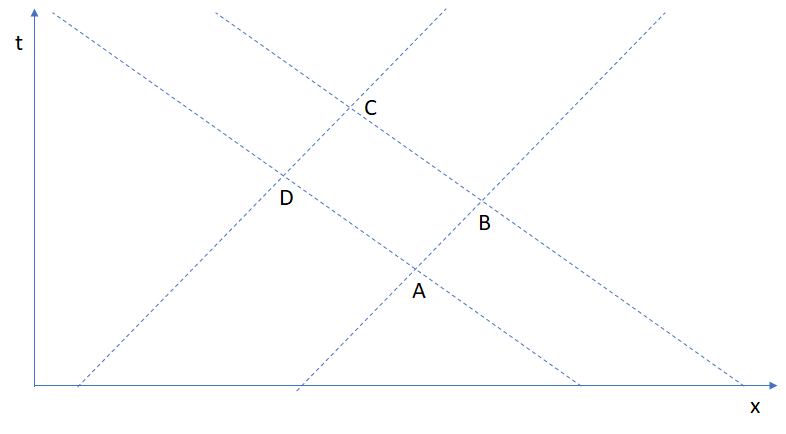
\includegraphics[scale=0.5]{s28_f1}
\caption{The parallelogram law.}
\label{s28f1}
\end{figure}

We will now solve the initial value problem $u_{tt} - u_{xx} = 0$ such that $u(x 0) = \varphi(x)$ and 
$u_t(x, 0) = \psi(x)$, where $\varphi \in C^2(\mathbb{R})$ and $\psi \in C^1(\mathbb{R})$. From equation 
\eqref{s28e2}, 
\begin{eqnarray}
u(x, 0) &=& g(x) + h(x) = \varphi(x) \label{s28e4} \\
u_t(x, 0) &=& -g^\prime(x) + h^\prime(x)  = \psi(x) \label{s28e5}
\end{eqnarray}
so that
\begin{eqnarray}
h^\prime(x) &=& \frac{1}{2}(\varphi^\prime(x) + \psi(x)) \label{s28e6} \\
g^\prime(x) &=& \frac{1}{2}(\varphi^\prime(x) - \psi(x)) \label{s28e7}
\end{eqnarray}
Integrating the above equations, we get
\begin{equation}\label{s28e8}
h(x) = \frac{1}{2}\left(\varphi(x) + \int_0^x\psi(s)ds\right) + c,
\end{equation}
where $c$ is a constant of integration. Substituting this equation in \eqref{s28e4} we get
\begin{equation}\label{s28e9}
g(x) = \frac{1}{2}\left(\varphi(x) - \int_0^x\psi(s)ds\right) - c.
\end{equation}
Using equations \eqref{s28e8} and \eqref{s28e9} in \eqref{s28e2}, we get
\[
u(x) = \frac{1}{2}\left(\varphi(x + t) + \int_0^{x+t}\psi(s)ds\right) + c +
\frac{1}{2}\left(\varphi(x - t) - \int_0^{x-t}\psi(s)ds\right) - c
\]
or
\begin{equation}\label{s28e10}
u(x) = \frac{1}{2}(\varphi(x+t) + \varphi(x-t)) + \frac{1}{2}\int_{x-t}^{x+t}\psi(s)ds.
\end{equation}
Equation \eqref{s28e10} is called the d'Alembert's solution of the one dimensional wave equation.

\begin{defn}\label{s28d1}
The spherical mean of a function $f : \mathbb{R}^n \rightarrow \mathbb{R}$ at a point $x \in \mathbb{R}^n$ is
defined as
\[
F(x; r) = \frac{1}{S(r, n)}\fint_{\partial B(x, r)} f(y)dS(y)
\]
where $S(r, n)$ is the surface area of the ball $B(x, r)$ or
\[
F_1(x; r) = \frac{1}{V(r, n)}\fint_{B(x, r)} f(y)dy
\]
\end{defn}

We will now show 
\begin{prop}\label{s28p1}
Let $u$ be a solution of the initial value problem $u_{tt} - u_{xx} = 0$ subject to the conditions $u = g, u_t = h$
on $\mathbb{R}^n \times \{t = 0\}$. Define
\begin{equation}\label{s28e11}
U(x; r, t) = \fint_{\partial B(x,r)}u(y, t)dS(y),
\end{equation}
where $x \in \mathbb{R}^n, r > 0, t > 0$. Then $U \in C^m(\bar{\mathbb{R}}_+ \times [0, \infty))$ and $U$ 
satisfies the Euler-Poisson-Darboux equation 
\begin{equation}\label{s28e12}
U_{tt} - U_{rr} - \frac{n - 1}{r}U_r = 0
\end{equation} 
in $\mathbb{R}_+ \times (0, \infty)$ and $U = G, U_t = H$ on $\mathbb{R}_+ \times \{t = 0\}$, where $G$ and $H$
are defined as
\begin{eqnarray}
G(x; r, t) &=& \fint_{\partial B(x,r)}g(y, t)dS(y) \label{s28e13}\\
H(x; r, t) &=& \fint_{\partial B(x,r)}h(y, t)dS(y) \label{s28e14}
\end{eqnarray}
\end{prop}
\begin{proof}
Let us first differentiate $U$ with respect to $r$. Since the domain of integration depends on $r$, we tranform the
problem so that it is over a ball of radius $1$ centred at the origin. Let $z = (y - x)/r$ or $y = x + rz$. Then
$dS(y) = r^{n-1}dS(z)$ and
\begin{eqnarray*}
U(x; r, t) &=& \fint_{\partial B(x,r)} u(y,t)dS(y) \\
 &=& \frac{1}{S(n, r)}\int_{\partial B(x,r)} u(y, t)dS(y) \\
 &=& \frac{1}{S(n, r)}\int_{\partial B(0,1)} u(x + rz, t)r^{n-1} dS(z) \\
 &=& \frac{1}{S(n, 1)}\int_{\partial B(0,1)} u(x + rz, t) dS(z) \\
 &=& \fint_{\partial B(0,1)} u(x + rz, t)dS(z)
\end{eqnarray*}
so that
\begin{eqnarray*}
U_r(x; r, t) &=& \fint_{\partial B(0, 1)}Du(x + rz; r, t)zdS(z) \\
 &=& \fint_{\partial B(x, r)} Du(y)\frac{y - x}{r}dS(y)
\end{eqnarray*}
The vector $(y - x)/r$ is a unit normal to the surface so that
\[
U_r(x; r, t) = \fint_{\partial B(x, r)} \pd{u}{n}dS(y) = \frac{1}{S(r, n)}\int \Delta u dy 
= \frac{r}{n}\frac{1}{V(r, n)}\int\Delta u dy
\]
or
\begin{equation}\label{s28e15}
U_r(x; r, t) = \frac{r}{n}\fint_{B(x,r)} \Delta u dy.
\end{equation}
We now proceed to find the second derivative of $U$ with respect to $r$. Before we do so, let us write $U_r$ in
full as
\[
U_r(x; r, t) = \frac{r}{n}\frac{1}{\alpha(n)r^n}\int_{B(x, r)}\Delta u dy,
\]
where we wrote $V(r, n) = \alpha(n)r^n$, $\alpha(n) = \pi^{n/2}/\Gamma(1 + n/2)$. Thus,
\begin{equation}\label{s28e16}
U_r(x; r, t) = \frac{1}{n\alpha(n)r^{n-1}}\int_{B(x, r)}\Delta u dy.
\end{equation}
Let us write the volume integral on the right hand side as
\[
U_r(x; r, t) = \frac{1}{n\alpha(n)r^{n-1}}\int_0^r d\rho\int_{\partial B(x,\rho)} \Delta u dy
\]
Now,
\[
\frac{1}{n\alpha(n)\rho^{n-1}}\int_{\partial B(x,\rho)} \Delta u dy = \fint \Delta u(y)dy
\]
so that
\[
r^{n-1}U_r(x; r, t) = \int_0^r \rho^{n-1} d\rho \fint_{\partial B(x,\rho)} \Delta u(y)dS(y)
\]
Differentiating with respect to $r$,
\[
(n-1)r^{n-2}U_r + r^{n-1}U_{rr} = 
\lim_{h\rightarrow 0} \frac{1}{h} \int_r^{r+h} \rho^{n-1} \fint_{\partial B(x,\rho)} \Delta u(y)dS(y)d\rho
\]
or
\[
(n-1)r^{n-2}U_r + r^{n-1}U_{rr} = r^{n-1} \fint_{\partial B(x,r)} \Delta u(y)dS(y)
\]
or
\[
(n-1)\frac{U_r}{r} + U_{rr} = \fint_{\partial B(x,r)} \Delta u(y)dS(y)
\]
Using \eqref{s28e15}, we get
\begin{equation}\label{s28e17}
U_{rr}(x;r,t) = \left(\frac{1}{n} - 1\right)\fint_{B(x,r)} \Delta u dy + \fint_{\partial B(x,r)} \Delta u(y)dS(y).
\end{equation}
In order to find out $U_{tt}$, let us start from \eqref{s28e16} and rearrange it as
\[
r^{n-1}U_r = \frac{1}{n\alpha(n)}\int_{B(x,r)}\Delta u dy
\]
Differentiating with respect to $r$, we get
\[
(n-1)r^{n-2}U_r + r^{n-1}U_{rr} = \frac{1}{n\alpha(n)}\frac{\partial}{\partial r}\int_{B(x,r)}\Delta u dy
\]
or
\[
(n-1)r^{n-2}U_r + r^{n-1}U_{rr} = \frac{1}{n\alpha(n)}\int_{\partial B(x,r)}\Delta u dS(y)
\]
Since $u$ solves the wave equation
\[
(n-1)r^{n-2}U_r + r^{n-1}U_{rr} = \frac{r^{n-1}}{n\alpha(n)r^{n-1}}\int_{\partial B(x,r)}u_{tt} dS(y)
\]
or
\begin{equation}\label{s28e18}
(n-1)r^{n-2}U_r + r^{n-1}U_{rr} = r^{n-1}\fint_{\partial B(x,r)}u_{tt}dS(y) = r^{n-1}U_{tt}
\end{equation}
Dividing both sides by $r^{n-1}$ we get the Euler-Poisson-Darboux equation.
\end{proof}

Before proceeding to use the Euler-Poisson-Darboux equation let us solve the wave equation for the half plane.
\begin{eqnarray}
u_{tt} - u_{xx} &=& 0  \text{ in } \mathbb{R}_+ \times (0, \infty) \label{s28e19} \\
u &=& g  \text{ on } \mathbb{R}_+ \times \{t = 0\} \label{s28e20} \\
u_t &=& h \text{ on } \mathbb{R}_+ \times \{t = 0\} \label{s28e21} \\
u &=& 0 \text{ on } \{x = 0\} \times (0, \infty) \label{s28e22}.
\end{eqnarray}
Let us extend functions $u, g, h$ to entire $\mathbb{R}$ by odd reflection. That is, define
\begin{equation}\label{s28e23}
\tilde{u}(x, t) = \begin{cases}
u(x, t) & (x \ge 0, t \ge 0) \\
-u(-x, t) & (x \le 0, t \ge 0)
\end{cases}
\end{equation}
\begin{equation}\label{s28e24}
\tilde{g}(x) = \begin{cases}
g(x) & (x \ge 0) \\
-g(-x) & (x \le 0)
\end{cases}
\end{equation}
\begin{equation}\label{s28e25}
\tilde{h}(x) = \begin{cases}
h(x) & (x \ge 0) \\
-h(-x) & (x \le 0)
\end{cases}
\end{equation}
Why do we need an odd extension? Because we want to satisfy \eqref{s28e22}. If we had considered an even extension 
then we would have had $u(x, t) = u(-x, t)$ at $x = 0$ but that would not have guaranteed us $u = 0$ on $x = 0$. 
If, instead, we were working with Neumann boundary condition $u_x = 0$ on $\{x = 0\} \times (0, \infty)$ we would 
have been forced to consider even extension.

Using the definitions \eqref{s28e24} to \eqref{s28e25} it is easy to conclude that the $\tilde{u}$ is a solution of 
the initial value problem,
\begin{eqnarray}
\tilde{u}_{xx} &=& \tilde{u}_{tt} \text{ in } \mathbb{R} \times (0, \infty) \label{s28e26} \\
\tilde{u} &=& \tilde{g} \text{ on } \mathbb{R} \times \{t = 0\} \label{s28e27} \\
\tilde{u} &=& \tilde{h} \text{ on } \mathbb{R} \times \{t = 0\} \label{s28e28}.
\end{eqnarray}
Note that after extending $u$ to the entire real line, we do not need the special condition at $x = 0$. Our choice 
of odd extension automatically gives it to us. We thus observe that $\tilde{u}$ satisfies the boundary value 
condition for which we have found d'Alembert's solution. Thus, using \eqref{s28e10} we get
\begin{equation}\label{s28e29}
\tilde{u}(x, t) = \frac{1}{2}(\tilde{g}(x+t) + \tilde{g}(x-t)) + \frac{1}{2}\int_{x-t}^{x+t}\tilde{h}(s)ds.
\end{equation}
If $x > t > 0$ then \eqref{s28e29}, written in terms of $u$ becomes
\begin{equation}\label{s28e30}
u(x, t) = \frac{1}{2}(g(x+t) + g(x-t)) + \frac{1}{2}\int_{x-t}^{x+t}h(s)ds.
\end{equation}
If $x < t$, $\tilde{g}(x-t) = -g(t-x)$ and $\tilde{h}(x-t) = -h(t-x)$ so that \eqref{s28e29} becomes
\begin{eqnarray*}
u(x,t) &=& \frac{1}{2}(g(x+t) - g(t-x)) + \frac{1}{2}\int_{x-t}^{x+t}\tilde{h}(s)ds \\
 &=& \frac{1}{2}(g(x+t) - g(t-x)) + \frac{1}{2}\int_{x-t}^{0}\tilde{h}(s)ds + 
 \frac{1}{2}\int_{0}^{x+t}\tilde{h}(s)ds
\end{eqnarray*}
In the term on the right hand side, we put $\tilde{h}(s) = -h(-s)$ and in the third term we put $\tilde{h}(s) =
h(s)$ so that 
\[
u(x,t) = \frac{1}{2}(g(x+t) - g(t-x))-\frac{1}{2}\int_{x-t}^{0}h(-s)ds+\frac{1}{2}\int_{0}^{x+t}h(s)ds.
\]
Using the transformation $s \mapsto -s$ in the second term we get
\[
u(x,t) = \frac{1}{2}(g(x+t)-g(t-x))+\frac{1}{2}\int_{t-x}^{0}h(-s)ds+\frac{1}{2}\int_{0}^{x+t}h(s)ds
\]
or
\[
u(x,t) = \frac{1}{2}(g(x+t)-g(t-x))-\frac{1}{2}\int_{0}^{t-x}h(-s)ds+\frac{1}{2}\int_{0}^{x+t}h(s)ds
\]
or
\begin{equation}\label{s28e31}
u(x,t) = \frac{1}{2}(g(x+t)-g(t-x)) + \frac{1}{2}\int_{t-x}^{x+t}h(s)ds
\end{equation}

We will now solve the Euler-Poisson-Darboux equation for $n=3$. We recall that the $U$ in it is related to the 
solution of the initial value problem $u_{tt} - \Delta u = 0$ in $\mathbb{R}^n \times (0, \infty)$ subject to the 
conditions $u = g$ and $_t = h$ on $\mathbb{R}^n \times \{t=0\}$. Let us consider the transformation $\tilde{U} := 
rU, \tilde{G} := rG, \tilde{H} := rH$, where $U, G, H$ are defined in equations \eqref{s28e11}, \eqref{s28e13} and 
\eqref{s28e14}. Differentiating $\tilde{U}$ with respect to $r$ twice we get
\begin{eqnarray*}
\tilde{U}_r &=& U + rU_r \\
\tilde{U}_{rr} &=& 2U_r + rU_{rr}
\end{eqnarray*}
Substituting in \eqref{s28e12} for $n=3$ we get $\tilde{U}_{tt} - \tilde{U}_{rr} = 0$ in $\mathbb{R}_+ \times 
(0, \infty)$. Since $U(x; r, 0) = G(x; r, 0)$ (because $u(\cdot, 0) = g(\cdot)$), we have $\tilde{U} = \tilde{G}$ 
on $\mathbb{R}_+ \times \{t=0\}$. For similar reason, we also have $\tilde{U}_t = \tilde{H}$ on $\mathbb{R}_+ 
\times\{t=0\}$. Finally, when $r = 0$, $\tilde{U}$ vanishes. Thus, $\tilde{U}$ solves the initial value problem
\begin{eqnarray*}
\tilde{U}_{tt} - \tilde{U}_{rr} &=& 0 \text{ in } \mathbb{R}_+ (0, \infty) \\
\tilde{U} &=& \tilde{G} \text{ on } \mathbb{R}_+ \times \{t=0\} \\
\tilde{U}_t &=& \tilde{H} \text{ on } \mathbb{R}_+ \times \{t=0\} \\
\tilde{U} &=& 0 \text{ on } \{r = 0\} \times (0, \infty)
\end{eqnarray*}
Comparing these equations with \eqref{s28e19} to \eqref{s28e22}, we see that $\tilde{U}$ is a solution of the one-
dimensional wave equation in the half-plane and therefore its solution for $0 \le r \le t$, by analogy with 
\eqref{s28e31} is
\begin{equation}\label{s28e32}
\tilde{U}(x; r, t) = \frac{1}{2}(\tilde{G}(t+r)-\tilde{G}(t-r)) + \frac{1}{2}\int_{t-r}^{t+r}\tilde{H}(s)ds
\end{equation}

Since $U(x; r, t)$ is the average of $u$ at $x$ over a ball of radius $r$, in the limit $r$ tends to $0$, 
$U(x; r,t)$ will become $u(x)$, that is
\begin{equation}\label{s28e33}
\lim_{r \rightarrow 0^+}U(x; r, t) = u(x, t)
\end{equation}
so that\begin{equation}\label{s28e34}
\lim_{r \rightarrow 0^+}\frac{\tilde{U}(x; r, t)}{r} = u(x, t).
\end{equation}
Using \eqref{s28e32} in \eqref{s28e34} we get
\[
u(x,t) = \frac{1}{2}\lim_{r \rightarrow 0^+}\frac{\tilde{G}(t+r)-\tilde{G}(t-r)}{r} + 
\lim_{r \rightarrow 0^+}\left(\frac{1}{2r}\int_{t-r}^{t+r}\tilde{H}(s)ds\right)
\]
or
\[
u(x,t) = \tilde{G}^\prime(x;t) + \tilde{H}(x;t)
\]
Since $\tilde{G} = tG$ and $\tilde{H} = tH$,
\begin{equation}\label{s28e35}
u(x,t) = \frac{\partial}{\partial t}\left(t\fint_{\partial B(x,t)}g(y, t)dS(y)\right) + 
t\fint_{\partial B(x,t)}h(y, t)dS(y)
\end{equation}
Since
\begin{equation}\label{s28e36}
\fint_{\partial B(x,t)}g(y, t)dS(y) = \fint_{\partial B(0,1)}g(x+tz, t)dS(z),
\end{equation}
the first term on the right hand side of \eqref{s28e36} is
\begin{eqnarray*}
\frac{\partial}{\partial t}\left(t\fint_{\partial B(0,1)}g(x+tz, t)dS(z)\right) &=& 
\fint_{\partial B(0,1)}g(x+tz, t)dS(z) \\
& & + t\fint_{\partial B(0,1)}zDg(x+tz, t)dS(z)
\end{eqnarray*}
Reverting back to $y$, and substituting in \eqref{s28e35}, we get
\[
u(x,t) = \fint_{\partial B(x,t)}g(y, t)dS(y) + \fint_{\partial B(0,1)} Dg(y)\cdot(y-x)dS(y) + 
t\fint_{\partial B(x,t)}h(y, t)dS(y)
\]
or
\begin{equation}\label{s28e37}
u(x,t) = \fint_{\partial B(x,t)} (th(y) + g(y) + Dg\cdot(y-x))dS(y).
\end{equation}
Equation \eqref{s28e37} is called \emph{Kirchhoff's formula} for the solution of the initial-value problem.

There is no transformation that can transform Euler-Poisson-Darboux equation for $n=2$ into a one-dimensional wave 
equation. Jacque Hadamard devised an ingenious technique, called the \emph{method of descent}, that uses the 
solution for $n=3$ dimensions to $n=2$. Let $u(x_1, x_2, t)$ solve $u_{tt} - \Delta u = 0$ in $\mathbb{R}^2 \times 
(0, \infty)$ subject to $u = g$ and $u_t = h$ on $\mathbb{R}^2 \times \{t=0\}$. Define $\tilde{u}: \mathbb{R}^3 
\times (0, \infty) \mapsto \mathbb{R}$ such that
\begin{equation}\label{s28e38}
\tilde{u}(x_1, x_2, x_3, t) := u(x_1, x_2, t).
\end{equation}
From the above definition it is clear that $\tilde{u}_{tt} = u_{tt}, \tilde{u}_{x_1x_1} = u_{x_1x_1}, 
\tilde{u}_{x_2x_2} = u_{x_2x_2}$. Further, $\tilde{u}_{x_3}$ and $\tilde{u}_{x_3x_3}$ are both zero. Therefore, if 
$u$ is a solution of the two dimensional wave equation then $\tilde{u}_{tt} - \Delta\tilde{u} = 0$ in $\mathbb{R}^3 
\times (0, \infty)$ and $\tilde{u} = \tilde{g}, \tilde{u}_t = \tilde{h}$ on $\mathbb{R}^3 \times \{t = 0\}$. Thus, 
$\tilde{u}$ is a solution of three dimensional wave equation and we can write it using \eqref{s28e35} as
\[
\tilde{u}(x,t) = \frac{\partial}{\partial t}\left(t\fint_{\partial B(x,t)}\tilde{g}(y, t)dS(y)\right) + 
t\fint_{\partial B(x,t)}\tilde{h}(y, t)dS(y)
\]
In particular, if we choose $x_3=0$ and write $\bar{x} = (x_1, x_2, 0)$ then
\begin{equation}
u(x_1, x_2, t) = \frac{\partial}{\partial t}\left(t\fint_{\partial B(\bar{x},t)}\tilde{g}(y_1, y_2, 0, t)
d\bar{S}(\bar{y})\right) + t\fint_{\partial B(\bar{x},t)}\tilde{h}(y_1,y_2,0, t)d\bar{S}(\bar{y}),
\end{equation}
where $d\bar{S}(\bar{y})$ is the two-dimensional surface measure on the ball centred at $\bar{x}$ and with radius 
$t$. We now transform the surface integral to a ``volume" integral on a disc centred around $\bar{x}$. A point 
$(y_1, y_2)$ on the disc maps to a point $f(y_1, y_2) = (y_1, y_2, \sqrt{t^2 - (x_1 - y_1)^2 - (x_1 - y_2)^2})$. We 
will compute the area element on the sphere in terms of the ``volume" element on the disc. It is the cross product 
$D_1f \times D_2f$
\[
\left(1, 0, \frac{x_1 - y_1}{\sqrt{t^2 - (x_1 - y_1)^2 - (x_1 - y_2)^2}}\right) \times 
\left(0, 1, \frac{x_1 - y_1}{\sqrt{t^2 - (x_1 - y_1)^2 - (x_1 - y_2)^2}}\right)
\]
or
\[
\left(-\frac{(x_1 - y_1)}{\sqrt{t^2 - |x - y|^2}}, -\frac{(x_2 - y_2)}{\sqrt{t^2 - |x - y|^2}}, 1\right)
\]
The magnitude of the cross product is
\[
|D_1f \times D_2f| = \left(1 + \frac{|x - y|}{\sqrt{t^2 - |x - y|^2}}\right)^{1/2} = \frac{t}{\sqrt{t^2 - 
|x - y|^2}}
\]
so that
\[
d\bar{S}(\bar{y}) = \frac{t}{\sqrt{t^2 - |x - y|^2}}dy_1dy_2 = \frac{t}{\sqrt{t^2 - |x - y|^2}}dy
\]
However, since both hemispheres map to the same disc, we must have
\begin{equation}\label{s28e40}
d\bar{S}(\bar{y}) = \frac{2t}{\sqrt{t^2 - |x - y|^2}}dy_1dy_2 = \frac{2t}{\sqrt{t^2 - |x - y|^2}}dy
\end{equation}
As an aside, we note that if $\gamma(y) = (t^2 - |y - x|^2)^{1/2}$ then we observe that
\[
|D_1f \times D_2f| = (1 + |D\gamma(y)|^2)^{1/2}.
\]
Coming back to \eqref{s28e40},
\[
\fint_{\partial B(\bar{x},t)}\bar{g}d\bar{S}(\bar{y}) = 
\frac{1}{4\pi t^2}\int_{\partial\bar{B}(\bar{x},t)}\bar{g}d\bar{S}(\bar{y}) = 
\frac{1}{2\pi t}\int_{B(x,t)}\frac{g(y)}{\sqrt{t^2 - |x - y|^2}}dy,
\]
where we recall that $x = (x_1, x_2)$ and $y = (y_1, y_2)$. Since the ``volume" of the ball $B(x,t)=\pi t^2$, we
can write the last integral as an average to get
\begin{equation}\label{s28e41}
\fint_{\partial B(\bar{x},t)}\bar{g}d\bar{S}(\bar{y}) = \frac{t}{2}\fint_{B(x,t)} \frac{g(y)}{\sqrt{t^2 - 
|x - y|^2}}dy.
\end{equation}
Using equation \eqref{s28e41} and the corresponding equation for $h$ in \eqref{s28e35}, we get
\begin{equation}\label{s28e42}
u(x,t)=\frac{\partial}{\partial t}\left(\frac{t^2}{2}\fint_{B(x,t)} \frac{g(y)}{\sqrt{t^2 - |x - y|^2}}dy\right) + 
\frac{t^2}{2}\fint_{B(0,1)} \frac{h(x)}{\sqrt{t^2 - |x - y|^2}}dy.
\end{equation}
In order to find the derivative in the first term we transform the variable of integration to $z = (y - x)/t$ to
get
\[
\frac{t^2}{2}\fint_{B(x,t)} \frac{g(y)}{\sqrt{t^2 - |x - y|^2}}dy = 
\frac{t}{2}\fint_{B(0,1)} \frac{g(x+tz)}{\sqrt{1 - |z|^2}}dz
\]
so that
\[
\frac{\partial}{\partial t}\left(\frac{t^2}{2}\fint_{B(x,t)} \frac{g(y)}{\sqrt{t^2 - |x - y|^2}}dy\right) =
\frac{1}{2}\fint_{B(0,1)} \frac{g(x+tz)}{\sqrt{1 - |z|^2}}dz + 
\frac{t}{2}\fint_{B(0,1)} \frac{z\cdot Dg(x+tz)}{\sqrt{1 - |z|^2}}dz.
\]
Reverting back to $y$,
\begin{eqnarray*}
\frac{\partial}{\partial t}\left(\frac{t^2}{2}\fint_{B(x,t)} \frac{g(y)}{\sqrt{t^2 - |x - y|^2}}dy\right) &=&
\frac{t}{2}\fint_{B(x,t)}\frac{g(y)}{\sqrt{t^2 - |x - y|^2}}dy + \\
\frac{t}{2}\fint_{B(x,t)}\frac{(y-x)\cdot Dg}{\sqrt{t^2 - |x - y|^2}}dy
\end{eqnarray*}
Using this equation in \eqref{s28e42},
\begin{equation}\label{s28e43}
u(x,t) = \frac{1}{2}\fint_{B(x,t)}\frac{tg(y) + t(y-x)\cdot Dg(y) + t^2h(y)}{\sqrt{t^2 - |x - y|^2}}dy.
\end{equation}
Equation \eqref{s28e43} is called \emph{Poisson's formula} for the two dimensional wave equation.

We will now solve the Euler-Poisson-Darboux equation for arbitrary dimensions treating even and odd space 
dimensions separately.

\subsection{Odd space dimensions}
We will find the following proposition useful.
\begin{prop}\label{s28p2}
Let $\phi: \mathbb{R} \rightarrow \mathbb{R}$ be $C^{k+1}$. Then
\begin{enumerate}
\item \begin{equation}\label{s28e44}
\left(\frac{d}{dr}\right)^2\left(\frac{1}{r}\frac{d}{dr}\right)^{k-1}\left(r^{2k-1}\phi(r)\right) = 
\left(\frac{1}{r}\frac{d}{dr}\right)^k\left(r^{2k}\td{\phi}{r}\right).
\end{equation}
\item \begin{equation}\label{s28e45}
\left(\frac{1}{r}\frac{d}{dr}\right)^{k-1}\left(r^{2k-1}\phi(r)\right) = 
\sum_{j=0}^{k-1}\beta^k_j r^{j+1}\left(\frac{d}{dr}\right)^{j}\phi,
\end{equation}
where $\beta^k_j$ are constants, independent of $r$.
\item $\beta^k_0 = (2k-1)!!$.
\end{enumerate}
\end{prop}
\begin{proof}
We will prove \eqref{s28e44} by induction on $k$. When $k=1$,
\[
\text{LHS}= \left(\frac{d}{dr}\right)^2(r\phi(r)) = 2\phi^\prime(r) + r\phi^{\prime\prime}(r).
\]
and
\[
\text{RHS} = \left(\frac{1}{r}\frac{d}{dr}\right)(r^2\phi^\prime(r)) = 2\phi^\prime(r) + r\phi^{\prime\prime}(r).
\]
Let the claim be true for $1 < m < k$. Consider
\begin{equation}\label{s28e46}
\left(\frac{d}{dr}\right)^2\left(\frac{1}{r}\frac{d}{dr}\right)^{m}\left(r^{2m+1}\phi(r)\right) =
\left(\frac{d}{dr}\right)^2\left(\frac{1}{r}\frac{d}{dr}\right)^{m-1}\left(r^{2m-1}\psi(r)\right),
\end{equation}
where
\begin{equation}\label{s28e47}
\psi(r) = (2m+1)\phi(r) + r\phi^\prime(r).
\end{equation}
Using induction hypothesis on the right hand side of \eqref{s28e46} we get
\begin{equation}\label{s28e48}
\left(\frac{d}{dr}\right)^2\left(\frac{1}{r}\frac{d}{dr}\right)^{m}\left(r^{2m+1}\phi(r)\right) =
\left(\frac{1}{r}\frac{d}{dr}\right)^m\left(r^{2m}\td{\psi}{r}\right).
\end{equation}
Using the definition of $\psi$,
\[
r^{2m}\td{\psi}{r} = \left(\frac{1}{r}\frac{d}{dr}\right)\left(r^{2m+1}\td{\phi}{r}\right)
\]
so that equation \eqref{s28e48} becomes
\[
\left(\frac{d}{dr}\right)^2\left(\frac{1}{r}\frac{d}{dr}\right)^{m}\left(r^{2m+1}\phi(r)\right) =
\left(\frac{1}{r}\frac{d}{dr}\right)^{m+1}\left(r^{2(m+1)-1}\td{\phi}{r}\right).
\]

Equation \eqref{s28e45} can also be proved by induction on $k$. For $k=1$, LHS = $r\phi(r)$ while
\[
\text{RHS} = \sum_{j=0}^0 \beta^1_0 r\phi(r) = r\phi(r),
\]
if $\beta^1_0 = 1$, which it is as will be shown in part three of the proposition. Let the claim be true for $1 < m 
< k$. Consider
\begin{equation}\label{s28e49}
\left(\frac{1}{r}\frac{d}{dr}\right)^m(r^{2m+1}\phi(r)) = 
\left(\frac{1}{r}\frac{d}{dr}\right)\left[\left(\frac{1}{r}\frac{d}{dr}\right)^{m-1}(r^{2m-1}\psi(r))\right],
\end{equation}
where $\psi(r) = r^2\phi(r)$. Using the induction hypothesis for the term in square brackets on the right hand
side of the above equation we get
\begin{equation}\label{s28e50}
\left(\frac{1}{r}\frac{d}{dr}\right)^m(r^{2m+1}\phi(r)) = 
\left(\frac{1}{r}\frac{d}{dr}\right)\left[\sum_{j=0}^{m-1}\beta^m_j r^{j+1}\left(\frac{d}{dr}\right)^j\psi\right]
\end{equation}
From the definition of $\psi$, we can conclude that 
\[
\left(\frac{d}{dr}\right)^j\psi = \begin{cases}
2r\phi(r) + r^2\phi^\prime(r) & \text{ for } j = 1 \\ 
2\alpha_j \left(\frac{d}{dr}\right)^{j-2}\phi + 
2jr\left(\frac{d}{dr}\right)^{j-1}\phi + r^2\left(\frac{d}{dr}\right)^j\phi & \text{ for } j \ge 2.
\end{cases}
\]
The numbers $\alpha_j$ are defined recursively as $\alpha_j = \alpha_{j-1} + j$ with $\alpha_1 = 1$. Thus,
\begin{equation}\label{s28e51}
\left(\frac{1}{r}\frac{d}{dr}\right)\left(r^{j+1}\frac{d^j\psi}{dr^j}\right) = 
6r\phi(r) + 6r^2\phi^{\prime}(r) + r^3\phi^{\prime\prime}(r)
\end{equation}
when $j = 1$ and 
\begin{eqnarray}
\left(\frac{1}{r}\frac{d}{dr}\right)\left(r^j\frac{d^j\psi}{dr^j}\right) &=&
2(j+1)\alpha_j r^{j-1}\frac{d^{j-2}\phi}{dr^{j-2}} + 
r^j(2\alpha_j + 2j(j+2))\frac{d^{j-1}\phi}{dr^{j-1}} + \nonumber \\
& & 3r^{j+1}(j+1)\frac{d^j\phi}{dr^j} + r^{2+j}\frac{d^{j+1}\phi}{dr^{j+1}} \label{s28e52}
\end{eqnarray}
when $j \ge 2$. Substituting equations \eqref{s28e51} and \eqref{s28e52} in \eqref{s28e50},
\begin{eqnarray*}
\left(\frac{1}{r}\frac{d}{dr}\right)^m(r^{2m+1}\phi(r)) &=& 
\beta^m_0 (6r\phi(r) + 6r^2\phi^{\prime}(r) + r^3\phi^{\prime\prime}(r)) + \\
& & \sum_{j=1}^{m-1}\beta^m_j\left(2(j+1)\alpha_j r^{j-1}\frac{d^{j-2}\phi}{dr^{j-2}} + 
r^j(2\alpha_j + 2j(j+2))\frac{d^{j-1}\phi}{dr^{j-1}}\right.\\ 
& & \left. + r^{j+1}(j+1)\frac{d^j\phi}{dr^j} + r^{2+j}\frac{d^{j+1}\phi}{dr^{j+1}}\right) \\
&=& \sum_{j=0}^{m+1}\beta^{m+1}_j r^{j+1}\frac{d^j\phi}{dr^j},
\end{eqnarray*}
where the constants $\beta^{m+1}_j$ are independent of $r$.

\noindent Lastly, in order to prove that $\beta_0^k = (2k-1)!!$ we just note that it emerges out of the term
\[
\left(\frac{1}{r}\frac{d}{dr}\right)^{k-1} r^{2k-1}.
\]
\end{proof}

Returning back to the wave equation, let $u$ solve the equation
\begin{eqnarray}
u_{tt} &=& \Delta u \text{ in } \mathbb{R}^n \times (0, \infty) \label{s28e53} \\
u &=& g \text{ on } \mathbb{R}^n \times \{t = 0\} \nonumber \\
u_t &=& h \text{ on } \mathbb{R}^n \times \{t = 0\} \nonumber
\end{eqnarray}
where $n = 2k + 1$ and $k \ge 2$. Let $u \in C^{2k+1}(\mathbb{R}^n \times (0,\infty))$ solve this initial value
problem. Then the function $U$ defined by \eqref{s28e11} is also in $C^{2k+1}(\mathbb{R}^2)$. Define
\begin{eqnarray}
\tilde{U}(r, t) &:=& \left(\frac{1}{r}\frac{\partial}{\partial r}\right)^{k-1}(r^{2k-1}U(x; r,t)) \label{s28e54} \\
\tilde{G}(r) &:=& \left(\frac{1}{r}\frac{\partial}{\partial r}\right)^{k-1}(r^{2k-1}G(x;r)) \label{s28e55} \\
\tilde{H}(r) &:=& \left(\frac{1}{r}\frac{\partial}{\partial r}\right)^{k-1}(r^{2k-1}H(x;r)) \label{s28e56}
\end{eqnarray}
then by definition of $U, G, H$ and the above three equations
\begin{eqnarray}
\tilde{U}(r, 0) &=& \tilde{G}(r) \label{s28e57} \\
\tilde{U}_t(r, 0) &=& \tilde{H}(r) \label{s28e58}
\end{eqnarray}

Analogous to the case of three dimensions, we show that
\begin{prop}\label{s28p3}
$\tilde{U}$ solves the one-dimensional wave equation. That is $\tilde{U}_{tt} - \tilde{U}_{rr} = 0$ in 
$\mathbb{R}_+ \times (0, \infty)$, $\tilde{U} = \tilde{G}$ and $\tilde{U}_t = \tilde{H}$ on $\mathbb{R}_+ \times
\{t = 0\}$ and $\tilde{U}(0, t) = 0$.
\end{prop}
\begin{proof}
From equation \eqref{s28e54},
\[
\tilde{U}_{rr} = 
\frac{\partial^2}{\partial r^2}\left(\frac{1}{r}\frac{\partial}{\partial r}\right)^{k-1}(r^{2k-1}U(x; r,t))
\]
From equation \eqref{s28e44},
\begin{eqnarray*}
\tilde{U}_{rr} &=& \left(\frac{1}{r}\frac{\partial}{\partial r}\right)^k\left(r^{2k}U_r\right) \\
 &=& \left(\frac{1}{r}\frac{\partial}{\partial r}\right)^{k-1}\left(2kr^{2k-2}U_r + r^{2k-1}U_{rr}\right) \\
 &=& \left(\frac{1}{r}\frac{\partial}{\partial r}\right)^{k-1}\left[r^{2k-1}\left(U_{rr} + 
 \frac{n-1}{r}U_r\right)\right],
\end{eqnarray*}
where we used the fact that $2k = n - 1$. From the Euler-Poisson-Darboux equation \eqref{s28e12}, 
\[
\tilde{U}_{rr} = \left(\frac{1}{r}\frac{\partial}{\partial r}\right)^{k-1}(r^{2k-1}U_{tt})
\]
From \eqref{s28e54}, we see that the right hand side is $\tilde{U}_{tt}$. Thus $\tilde{U}$ satisfies the one-
dimensional wave equation. Let us now check if it also satisfies the boundary conditions. Using \eqref{s28e45},
we can write $\tilde{U}(r,t)$ as
\begin{equation}\label{s28e59}
\tilde{U}(r,t) = \sum_{j=0}^{k-1}\beta^k_j r^{j+1}\frac{\partial^j U}{\partial r^j}.
\end{equation}
Since $\beta_k^j$ are all constants and the $U$ is in $C^{2k+1}$ , $U(0, t) = 0$. The other two boundary conditions
follow from the definitions of $U, G, H$ and equations \eqref{s28e54} to \eqref{s28e56}.
\end{proof}

Since $\tilde{U}$ satisfies the one-dimensional wave equation, it can be expressed as d'Alembert's solution
\eqref{s28e10} 
\begin{equation}\label{s28e60}
\tilde{U}(r,t) = \frac{\tilde{G}(t+r) - \tilde{G}(t-r)}{2} + \frac{1}{2}\int_{t-r}^{t+r}\tilde{H}(y)dy.
\end{equation}
We are interested in getting a solution to equation \eqref{s28e53}. Therefore, we need a relationship between
$\tilde{U}$ and $u$. From equation \eqref{s28e59},
\[
\frac{\tilde{U}(r,t)}{r} = \sum_{j=0}^{k-1}\beta^k_j r^{j}\frac{\partial^j U}{\partial r^j}.
\]
so that
\[
\lim_{r \rightarrow 0}\frac{\tilde{U}(r,t)}{r} = \lim_{r\rightarrow 0} \beta^k_0 U(x; r, t) = \beta^k_0 u(x,t)
\]
or
\begin{equation}\label{s28e61}
u(x,t) = \lim_{r \rightarrow 0} \frac{\tilde{U}(r,t)}{\beta^k_0 r}.
\end{equation}
From equations \eqref{s28e60} and \eqref{s28e61},
\[
u(x,t) = \frac{\tilde{G}^\prime(t) + \tilde{H}(t)}{\beta^k_0}
\]
From part 3 of proposition \ref{s28p2}, $\beta_0^k = (2k-1)!!$. Since $n = 2k+1$, $\beta_0^k = (n-2)!!$. From
\eqref{s28e56}, 
\[
\tilde{H}(t) = \left(\frac{1}{t}\frac{\partial}{\partial t}\right)^{(n-3)/2}(t^{n-2}H(x,t))
\]
so that using \eqref{s28e13}, we get
\begin{equation}\label{s28e62}
\tilde{H}(t) = \left(\frac{1}{t}\frac{\partial}{\partial t}\right)^{(n-3)/2}
\left(t^{n-2}\fint_{\partial B(x,r)}h(y, t)dS(y)\right)
\end{equation}
Similarly,
\begin{equation}\label{s28e63}
\tilde{G}^\prime(t) = \frac{\partial}{\partial t}\left(\frac{1}{t}\frac{\partial}{\partial t}\right)^{(n-3)/2}
\left(t^{n-2}\fint_{\partial B(x,r)}h(y, t)dS(y)\right)
\end{equation}
Substituting equations \eqref{s28e62} and \eqref{s28e63} in \eqref{s28e61} we get
\begin{eqnarray}
u(x,t) &=& \frac{1}{(n-2)!!}\left[\frac{\partial}{\partial t}\left(\frac{1}{t}\frac{\partial}{\partial t}
\right)^{(n-3)/2}\left(t^{n-2}\fint_{\partial B(x,t)}gdS\right)\right. + \nonumber \\
& & \left.\left(\frac{1}{t}\frac{\partial}{\partial t}\right)^{(n-3)/2}\left(t^{n-2}
\fint_{\partial B(x,r)}h(y, t)dS(y)\right)\right] \label{s28e64}
\end{eqnarray}
Equation \eqref{s28e64} is the solution to the initial value problem of \eqref{s28e53} when $n=2k+1$.

\subsection{Even space dimensions}
We will use Hadamard's method of descent to derive the explicit solution of the wave equation for even space
dimensions. Once again, define 
\begin{equation}\label{s28e65}
\bar{u}(x_1, \ldots, x_{n+1}, t) := u(x_1, \ldots, x_n, t).
\end{equation}
Define $\bar{g}$ and $\bar{h}$ similarly. Assume that $\bar{u}$ solves the wave equation in $\mathbb{R}^{n+1}
\times (0, \infty)$ with initial conditions $\bar{u} = \bar{g}$ and $\bar{u}_t = \bar{h}$ on $\mathbb{R}^{n+1}
\times \{0\}$. Now fix $x \in \mathbb{R}^n$ and $\bar{x} = (x, 0)$. Using \eqref{s28e64},
\begin{eqnarray}
u(x,t) &=& \frac{1}{(n-2)!!}\left[\frac{\partial}{\partial t}\left(\frac{1}{t}\frac{\partial}{\partial t}
\right)^{(n-2)/2}\left(t^{n-1}\fint_{\partial\bar{B}(x,t)}\bar{g}d\bar{S}\right)\right. + \nonumber \\
& & \left.\left(\frac{1}{t}\frac{\partial}{\partial t}\right)^{(n-2)/2}\left(t^{n-1}
\fint_{\partial\bar{B}(x,t)}\bar{h}(y, t)d\bar{S}(y)\right)\right]. \label{s28e66}
\end{eqnarray}
Note that $\bar{B}(x,t)$ is a ball in $\mathbb{R}^{n+1}$ with centre $x$ and radius $t$ and $d\bar{S}$ is the
$n$-dimensional surface measure on $\partial\bar{B}(x,t)$. From equations \eqref{s16e7}, \eqref{s16e10} and
\eqref{s16e11}, $S(n+1, t) = (n+1)V(n+1,1)t^n$ so that
\[
\fint_{\partial\bar{B}(x,t)}\bar{g}d\bar{S} = \frac{1}{(n+1)V(n+1,1)t^n}\int_{\partial\bar{B}(x,t)}\bar{g}d\bar{S}.
\]
Transforming the integral to the $n$-disk,
\[
\fint_{\partial\bar{B}(x,t)}\bar{g}d\bar{S} = \frac{2}{(n+1)V(n+1,1)t^n}
\int_{\partial\bar{B}(x,t)}\bar{g}(1 + |D\gamma(y)|^2)^{1/2}dy,
\]
where $\gamma(y) = \sqrt{t^2 - |x - y|^2}$ and the factor of $2$ arising due to contribution from each hemisphere.
Since 
\[
D\gamma(y) = \frac{t}{\sqrt{t^2 - |x - y|^2}}
\]
we have
\[
\fint_{\partial\bar{B}(x,t)}\bar{g}d\bar{S} = \frac{2}{(n+1)V(n+1,1)t^{n-1}}
\int_{\partial\bar{B}(x,t)}\frac{\bar{g}}{\sqrt{t^2 - |x - y|^2}}dy.
\]
Writing the integral on the right hand side and an average,
\[
\fint_{\partial\bar{B}(x,t)}\bar{g}d\bar{S} = \frac{2V(n,1)t^n}{(n+1)V(n+1,1)t^{n-1}}
\fint_{\partial\bar{B}(x,t)}\frac{\bar{g}}{\sqrt{t^2 - |x - y|^2}}dy.
\]
or
\begin{equation}\label{s28e67}
\fint_{\partial\bar{B}(x,t)}\bar{g}d\bar{S} = \frac{2V(n,1)t}{(n+1)V(n+1,1)}
\fint_{\partial\bar{B}(x,t)}\frac{\bar{g}}{\sqrt{t^2 - |x - y|^2}}dy.
\end{equation}
Since $V(n, 1) = \pi^{n/2}/\Gamma(1 + n/2)$, 
\[
\frac{V(n,1)}{V(n+1,1)} = \frac{1}{\sqrt{\pi}}\frac{\Gamma((n+3)/2)}{\Gamma((n+2)/2)}
\]
Since $n$ is even, $n+3$ is odd and therefore the expansion of the numerator will end with $\Gamma(1/2) = 
\sqrt{\pi}$. Using the fact that $\Gamma(z) = (z-1)\Gamma(z-1)$, we get
\[
\frac{V(n,1)}{V(n+1,1)} = \frac{(n+1)(n-1) \cdots 3}{n(n-2)(n-4) \cdots 2}
\]
and hence
\begin{equation}\label{s28e68}
\frac{V(n,1)}{(n+1)V(n+1)} = \frac{(n-1)!!}{n!!}.
\end{equation}
From equations \eqref{s28e67} and \eqref{s28e68}, we get
\begin{equation}\label{s28e69}
\fint_{\partial\bar{B}(x,t)}\bar{g}d\bar{S} = \frac{2t(n-1)!!}{n!!}
\fint_{\partial B(x,t)}\frac{g}{\sqrt{t^2 - |x - y|^2}}dy.
\end{equation}
Substituting \eqref{s28e69} and the analogous equation for $\bar{h}$ in \eqref{s28e66}, we get the explicit form
of the solution of the wave equation in $n$ dimensions as
\begin{eqnarray}
u(x,t) &=& \frac{1}{n!!}\left[\frac{\partial}{\partial t}\left(\frac{1}{t}\frac{\partial}{\partial t}
\right)^{(n-2)/2}\left(t^n\fint_{B(x,t)}\frac{g}{\sqrt{t^2 - |x - y|^2}}dy\right)\right. + \nonumber \\
& & \left.\left(\frac{1}{t}\frac{\partial}{\partial t}\right)^{(n-2)/2}\left(t^n
\fint_{B(x,t)}\frac{h}{\sqrt{t^2 - |x - y|^2}}dy\right)\right]. \label{s28e70}
\end{eqnarray}
Comparing equations \eqref{s28e64} and \eqref{s28e70} brings out the key difference between the solution of the
wave equation in odd and even dimensions. When the number of spatial dimensions is odd the data $g$ and $h$ at
$x \in \mathbb{R}^n$ determine the solution $u$ only on the boundary $\partial B(x, t)$. On the other hand, when
the number of spatial dimensions is even, data in the entire ball $B(x, t)$ determine the solution on its boundary.
Thus, Huygen's principle is valid in odd spatial dimensions but not in even spatial dimensions.

Equations \eqref{s28e64} and \eqref{s28e70} give the explicit solutions of the wave equations in any dimensions. 
Yet we haven't confirmed that they indeed solve the wave equation and have the right continuity properties. The
next two theorems will accomplish this task.

\begin{thm}\label{s28t1}
Let $n \ge 3$ be an odd integer, $g \in C^{m+1}(\mathbb{R}^n), h \in C^n(\mathbb{R}^n)$ for $m = (n + 1)/2$. Then
$u$ defined by \eqref{s28e64} has the following properties.
\begin{enumerate}
\item $u \in C^2(\mathbb{R}^n \times (0, \infty)$,
\item $u_{tt} - \Delta u = 0$ in $\mathbb{R}^n \times (0, \infty)$,
\item For all $x \in \mathbb{R}^n, t > 0$, $u(x, t) \rightarrow g(x_0)$ and $u_t(x, t) \rightarrow h(x_0)$ in the
limit $x \rightarrow x_0, t \rightarrow 0+$.
\end{enumerate}
\end{thm}
\begin{proof}
Using equations \eqref{s28e14} and \eqref{s28e15}, we can write \eqref{s28e64} as
\begin{equation}\label{s28e71}
u(x,t) = \frac{1}{(n-2)!!}\left[\frac{\partial}{\partial t}
\left(\frac{1}{t}\frac{\partial}{\partial t}\right)^{(n-3)/2}(t^{n-2}G(x; t,t)) +
\left(\frac{1}{t}\frac{\partial}{\partial t}\right)^{(n-3)/2}(t^{n-2}H(x; t,t))\right]
\end{equation}
Using \eqref{s28e44},
\begin{equation}\label{s28e72}
u_{tt}(x,t) = \frac{1}{(n-2)!!}\left[\frac{\partial}{\partial t}
\left(\frac{1}{t}\frac{\partial}{\partial t}\right)^{(n-1)/2}(t^{n-1}G_t(x; t,t)) +
\left(\frac{1}{t}\frac{\partial}{\partial t}\right)^{(n-1)/2}(t^{n-1}H_t(x; t,t))\right]
\end{equation}
Let us now calculate $G_t$ and $H_t$. From \eqref{s28e13},
\[
G(x;t,t) = \fint_{\partial B(x,t)}g(y,t)dS(y) = \frac{1}{S(n,t)}\int_{\partial B(x,t)} g(y,t)dS(y)
\]
Introduce a new variable $z = (y - x)/t$ so that $dS(z) = dS(y)/t^{n-1}$ and
\[
G(x;t,t) = \frac{1}{S(n,1)}\int_{\partial B(0,1)} g(x + tz) dS(z)
\]
so that
\[
G_t(x;t,t) = \frac{1}{S(n,1)}\int_{\partial B(0,1)} z\cdot Dg dS(z) = 
\frac{1}{S(n,r)}\int_{\partial B(x,t)} \frac{(y - x)}{r}\cdot Dg dS(y)
\]
Since $(y - x)/r$ is a unit normal to the ball $\partial B(x,r)$, we can use Gauss' theorem to get
\[
G_t(x;t,t) = \frac{t}{nV(n,t)}\int_{B(x,t)} \Delta g dy
\]
or
\begin{equation}\label{s28e73}
G_t(x;t,t) = \frac{t}{n}\fint_{B(x,t)} \Delta g dy
\end{equation}
Similarly,
\begin{equation}\label{s28e74}
H_t(x;t,t) = \frac{t}{n}\fint_{B(x,t)} \Delta h dy
\end{equation}
From \eqref{s28e73},
\[
t^{n-1}G_t = \frac{t^n}{n}\fint_{B(x,t)} \Delta g dy = \frac{t^n}{nV(n,t)}\int_{B(x,t)}\Delta g dy =
\frac{1}{nV(n,1)}\int_{B(x,t)}\Delta g dy
\]
so that
\[
\frac{\partial}{\partial t}(t^{n-1}G_t) = \frac{1}{nV(n,1)}\frac{\partial}{\partial t}\int_{B(x,t)}\Delta g dy
\]
Split the volume integral on the right hand side as
\[
\frac{\partial}{\partial t}(t^{n-1}G_t) = \frac{1}{nV(n,1)}\frac{\partial}{\partial t}
\left(\int_0^t\int_{\partial B(x,\rho)} \Delta g dS(y)d\rho\right)
\]
Using the first principles to compute the derivative on the right hand side,
\[
\frac{\partial}{\partial t}(t^{n-1}G_t) = \frac{1}{nV(n,1)}\lim_{h\rightarrow 0}
\left(\int_t^{t+h}\int_{\partial B(x,\rho)} \Delta g dS(y)d\rho\right)
\]
or
\[
\frac{\partial}{\partial t}(t^{n-1}G_t) = \frac{1}{nV(n,1)}\int_{\partial B(x,t)} \Delta g dS(y)
\]
or
\[
\frac{1}{t}\frac{\partial}{\partial t}(t^{n-1}G_t) = \frac{1}{nV(n,1)t}\int_{\partial B(x,t)} \Delta g dS(y)
\]
and hence
\begin{equation}\label{s28e75}
\left(\frac{1}{t}\frac{\partial}{\partial t}\right)^{(n-1)/2}(t^{n-1}G_t(x; t,t)) = 
\frac{1}{nV(n,1)}\left(\frac{1}{t}\frac{\partial}{\partial t}\right)^{(n-3)/2}
\frac{1}{t}\int_{\partial B(x,t)} \Delta g dS(y)
\end{equation}
Similarly,
\begin{equation}\label{s28e76}
\left(\frac{1}{t}\frac{\partial}{\partial t}\right)^{(n-1)/2}(t^{n-1}H_t(x; t,t)) = 
\frac{1}{nV(n,1)}\left(\frac{1}{t}\frac{\partial}{\partial t}\right)^{(n-3)/2}
\frac{1}{t}\int_{\partial B(x,t)} \Delta h dS(y)
\end{equation}
Substituting \eqref{s28e75} and \eqref{s28e76} in \eqref{s28e72},
\begin{eqnarray}
u_{tt}(x,t) &=& \frac{1}{nV(n,1)(n-2)!!}\left[\frac{\partial}{\partial t}
\left(\frac{1}{t}\frac{\partial}{\partial t}\right)^{(n-3)/2}\frac{1}{t}\int_{\partial B(x,t)} \Delta g dS(y) 
\right. \nonumber \\
& & + \left.
\left(\frac{1}{t}\frac{\partial}{\partial t}\right)^{(n-3)/2}\frac{1}{t}\int_{\partial B(x,t)}\Delta hdS(y)\right]
\label{s28e77}
\end{eqnarray}
From \eqref{s28e13}, once again,
\[
\Delta G(x; t,t) = \Delta_x \frac{1}{S(n,t)}\int_{\partial B(x,t)}g(y,t)dS(y) 
\]
Introduce a new variable $z = y - x$ so that
\[
\Delta G(x;t,t) = \frac{1}{S(n,t)}\Delta_x\int_{\partial B(0,t)} g(x + z, t)dS(z) = 
\frac{1}{S(n,t)}\int_{\partial B(0,t)} \Delta_x g(x + z, t)dS(z) 
\]
or
\[
\Delta G(x;t,t) = \frac{1}{S(n,t)}\int_{\partial B(0,t)} \Delta_z g(x + z, t)dS(z) = 
\fint_{\partial B(x,t)} \Delta_y g(y, t)dS(y)
\]
We can carry out the same steps for $H$ to get
\begin{eqnarray}
\Delta G(x;t,t) &=& \fint_{\partial B(x,t)} \Delta g(y, t)dS(y) \label{s28e78} \\
\Delta H(x;t,t) &=& \fint_{\partial B(x,t)} \Delta h(y, t)dS(y) \label{s28e79}
\end{eqnarray}
Substituting equations \eqref{s28e78} and \eqref{s28e79} in \eqref{s28e77} we get
\begin{eqnarray*}
u_{tt}(x,t) &=& \frac{1}{nV(n,1)(n-2)!!}\left[\frac{\partial}{\partial t}
\left(\frac{1}{t}\frac{\partial}{\partial t}\right)^{(n-3)/2}\frac{S(n,t)}{t}\Delta G(x;t,t) 
\right.  \\
& & + \left.
\left(\frac{1}{t}\frac{\partial}{\partial t}\right)^{(n-3)/2}\frac{S(n,t)}{t}\Delta H(x;t,t)\right]
\end{eqnarray*}
Now,
\[
S(n,t) = \frac{n}{t}V(n,t) = \frac{n}{t}V(n,1)t^n
\]
so that
\begin{eqnarray*}
u_{tt}(x,t) &=& \frac{1}{(n-2)!!}\left[\frac{\partial}{\partial t}
\left(\frac{1}{t}\frac{\partial}{\partial t}\right)^{(n-3)/2}t^{n-2}\Delta G(x;t,t) 
\right.  \\
& & + \left.
\left(\frac{1}{t}\frac{\partial}{\partial t}\right)^{(n-3)/2}t^{n-2}\Delta H(x;t,t)\right]
\end{eqnarray*}
or,
\begin{eqnarray*}
u_{tt}(x,t) &=& \Delta\left\{\frac{1}{(n-2)!!}\left[\frac{\partial}{\partial t}
\left(\frac{1}{t}\frac{\partial}{\partial t}\right)^{(n-3)/2}t^{n-2} G(x;t,t) 
\right.\right.  \\
& & + \left.\left.
\left(\frac{1}{t}\frac{\partial}{\partial t}\right)^{(n-3)/2}t^{n-2} H(x;t,t)\right]\right\}
\end{eqnarray*}
From equation \eqref{s28e71} we get $u_{tt} = \Delta u$. This also shows that $u \in C^2(\mathbb{R}^n \times 
(0,\infty))$.

Since $n=2k+1$, let us write \eqref{s28e71} in terms of $k$ so that
\[
u(x,t) = \frac{1}{(2k-1)!!}\left[\frac{\partial}{\partial t}
\left(\frac{1}{t}\frac{\partial}{\partial t}\right)^{k-1}(t^{2k-1}G(x; t,t)) +
\left(\frac{1}{t}\frac{\partial}{\partial t}\right)^{k-1}(t^{2k-1}H(x; t,t))\right]
\]
Using equation \eqref{s28e45}, 
\begin{equation}\label{s28e80}
u(x,t) = \frac{1}{(2k-1)!!}\left[\frac{\partial}{\partial t}\sum_{j=0}^{k-1}\beta_j^kt^{j+1}\frac{d^jG}{dt^j}
+ \sum_{j=0}^{k-1}\beta_j^kt^{j+1}\frac{d^jH}{dt^j}\right]
\end{equation}
or, using part (3) of proposition \ref{s28p2},
\[
u(x,t) = G + t\td{G}{t} + \frac{1}{(2k-1)!!}\left[
\frac{\partial}{\partial t}\sum_{j=1}^{k-1}\beta_j^kt^{j+1}\frac{d^jG}{dt^j}
+ \sum_{j=0}^{k-1}\beta_j^kt^{j+1}\frac{d^jH}{dt^j}\right]
\]
In the limit $t \rightarrow 0$, only the first term on the right hand side survives. This is because all the 
derivatives of $G$ and $H$ up to order $k-1$ are known to exist. The limit of the right hand side is thus $g(x)$. 
Taking the derivative of \eqref{s28e80} with respect to $t$,
\[
\frac{1}{(2k-1)!!}\left[\frac{\partial^2}{\partial t^2}\sum_{j=0}^{k-1}\beta_j^kt^{j+1}\frac{d^jG}{dt^j}
+ \frac{\partial}{\partial t}\sum_{j=0}^{k-1}\beta_j^kt^{j+1}\frac{d^jH}{dt^j}\right]
\]
Once again, the only surviving term is $H$, whose limit as $t \rightarrow 0$ is $h(x)$. Note that the term $G_t$
also tends to zero because of \eqref{s28e73}.
\end{proof}

The analogous theorem for even spatial dimensions is
\begin{thm}\label{s28t2}
Let $n \ge 3$ be an even integer, $g \in C^{m+1}(\mathbb{R}^n), h \in C^n(\mathbb{R}^n)$ for $m = (n + 2)/2$. Then
$u$ defined by \eqref{s28e70} has the following properties.
\begin{enumerate}
\item $u \in C^2(\mathbb{R}^n \times (0, \infty)$,
\item $u_{tt} - \Delta u = 0$ in $\mathbb{R}^n \times (0, \infty)$,
\item For all $x \in \mathbb{R}^n, t > 0$, $u(x, t) \rightarrow g(x_0)$ and $u_t(x, t) \rightarrow h(x_0)$ in the
limit $x \rightarrow x_0, t \rightarrow 0+$.
\end{enumerate}
\end{thm}

\subsection{Nonhomogeneous problem}
Consider the Cauchy problem for the nonhomogeneous wave equation,
\begin{equation}\label{s28e81}
u_{tt} - \Delta u = f \text{ in } \mathbb{R}^n \times (0, \infty)
\end{equation}
subject to the initial conditions
\begin{equation}\label{s28e82}
u = 0, u_t = 0 \text{ on } \mathbb{R}^n \times \{0\}.
\end{equation}
Introduce the function $v = u(x,t;s)$ satisfying the initial value problem $v_{tt} - \Delta v = 0$ in $\mathbb{R}^n
\times [s, \infty)$ subject to the initial conditions $v(x,t;s) = 0, v_t(x,t;s) = f(s)$ on $\mathbb{R}^n \times
\{t=s\}$. If 
\begin{equation}\label{s28e83}
u(x, t) = \int_0^t v(x,t;s)ds
\end{equation}
then \emph{Duhamel's principle} asserts that $u$ solves the problem of equations \eqref{s28e81} and \eqref{s28e82}.
We will prove it in the following theorem.
\begin{thm}\label{s28t3}
Assume that $n \ge 2$, $f \in C^{\lceil{n/2}+1\rceil}(\mathbb{R}^n \times (0, \infty)$. For $u$ defined by 
\eqref{s28e83},
\begin{enumerate}
\item $u \in C^2(\mathbb{R}^n$,
\item $u_{tt} - \Delta u = f$ in $\mathbb{R}^n \times (0, \infty)$,
\item $u(x,t) \rightarrow 0$ and $u_t(x,t) \rightarrow 0$ as $(x,t) \rightarrow (x_0, 0+)$ for every $x_0 \in
\mathbb{R}^n$.
\end{enumerate}
\end{thm}
\begin{proof}
Irrespective of whether $n$ is even or odd, theorems \ref{s28t1} and \ref{s28t2}, $v$ is twice differentiable in $
[s, \infty)$ for all $s > 0$ and $x \in \mathbb{R}^n$. Since the first derivative of $u$ is $v$, $u$ is also 
guaranteed to be twice differentiable.

From equation \eqref{s28e83}, using proposition \ref{s27p3}
\[
u_t(x,t) = v(x,t;t) + \int_0^t v_t(x,t;s)ds 
\]
Since $v(x,t;s) = 0$ when $t=s$ (refer to the initial conditions on the $v$-problem), we have
\begin{equation}\label{s28e84}
u_t(x,t) = \int_0^t v_t(x,t;s)ds
\end{equation}
Similarly,
\[
u_{tt}(x,t) = v_t(x,t;t) + \int_0^t v_{tt}(x,t;s)ds = f(x,t) + \int_0^t v_{tt}(x,t;s)ds
\]
Taking the laplacian of $u$ is quite straightforward,
\[
\Delta u = \int_0^t \delta v(x,t;s)ds = \int_0^t v_{tt}(x,t;s)ds
\]
so that $u_{tt} - \Delta u = f(x,t)$.

Finally, $u(x,0) = 0$ by its definition and $u_t(x,0) = 0$ be \eqref{s28e84}.
\end{proof}

Lastly, we show how the formula for retarted potential naturally arises in the Duhamel's principle applied to the
inhomogeneous wave equation in three dimensions. The solution $v$ of the corresponding homogeneous equation is
given by Kirchhoff's formula \eqref{s28e37} but with initial conditions $v(x, 0) = 0$ and $v_t(x,t) = f$. Thus,
in Kirchhoff's formula, $g = 0$ and $h = f$. The solution of the homogeneous problem is
\[
v(x,t;s)=\fint_{\partial B(x,t-s)}(t-s)fdS(y)
\]
in $\mathbb{R}^n \times (s,\infty)$. Therefore, the solution of the homogeneous equation is
\[
u(x,t) = \int_0^t\fint_{\partial B(x,t-s)}(t-s)f(y,s)dS(y)ds = 
\frac{1}{4\pi}\int_0^t\int_{\partial B(x,t-s)}\frac{f(y,s)}{t - s}dS(y)ds
\]
Introduce the variable $r = t - s$ so that
\[
u(x,t) = \frac{1}{4\pi}\int_0^t\int_{\partial B(x,r)}\frac{f(y, t-r)}{r}dS(y)dr
= \frac{1}{4\pi}\int_{B(x,t)}\frac{f(y, t - |x - y|)}{|y - x|}dy.
\]

\section{Problems}\label{s29}
\begin{enumerate}
\setlength{\leftmargin}{0pt}
\item Let $u, v \in C^2(\bar{U})$ prove the following identities using the Green-Gauss theorem \ref{s30t1}
\begin{equation}\label{s29e1}
\int_U v_{x_i} dx = \int_{\partial U} vn_i dS(x)
\end{equation}
If we apply this formula to $uv$, we get
\[
\int_U (uv)_{x_i} dx = \int_{\partial U} uv n_i dS(x)
\]
or
\[
\int_U uv_{x_i} dx + \int_U u_{x_i}v dx = \int_{\partial U} uv n_i dS(x)
\]
from which we get the integration by parts formula
\begin{equation}\label{s29e2}
\int_U u_{x_i} v dx = -\int_U uv_{x_i}dx + \int_{\partial U} uv n_i dS(x).
\end{equation}
\begin{enumerate}
\setlength{\leftmargin}{0pt}
\item 
\begin{equation}\label{s29e3}
\int_U\Delta u dx = \int_{\partial U}n \cdot Du dS(x) 
\end{equation}
Use $v = u_{x_i}$ in \eqref{s29e1} and the fact that $\Delta u = \sum_{i=1}^nu_{x_ix_i}$. 
\item 
\begin{equation}\label{s29e4}
\int_U v\Delta u dx = -\int_U Du\cdot Dv dx + \int_{\partial U}v n\cdot Du dS(x)
\end{equation}
Use the mapping $u \mapsto u_{x_i}$ in \eqref{s29e2} to get
\[
\int_U u_{x_ix_i} v dx = -\int_U u_{x_i}v_{x_i}dx + \int_{\partial U} u_{x_i}v n_i dS(x).
\]
Summing $i$ from $1$ to $n$ gives \eqref{s29e4}.
\item
\begin{equation}\label{s29e5}
\int_U(u \Delta v - v \Delta u) dx = \int_{\partial U}(u\;Dv - v\;Du)\cdot n dS.
\end{equation}
Interchanging $u$ and $v$ in equation \eqref{s29e4},
\begin{equation}\label{s29e6}
\int_U u\Delta v dx = -\int_U Du\cdot Dv dx + \int_{\partial U}u n\cdot Dv dS(x)
\end{equation}
Subtracting \eqref{s29e4} from \eqref{s29e6} gives \eqref{s29e5}.
from which we 
\end{enumerate}

\item Let $\Phi$ be the fundamental solution of the Laplace equation. Prove that $\Phi$ and $\Phi_{x_i}$ are
locally integrable but $\Phi_{x_ix_j}$ is not.

Solution: We will prove the assertion separately for $n=2$ and $n > 2$. For $n=2$,
\begin{eqnarray*}
\Phi(r) &=& -\frac{1}{2\pi}\ln r \\
\Phi_{x_i}(r) &=& -\frac{1}{2\pi}\frac{x_i}{r} \\
\Phi_{x_ix_j}(r) &=& -\frac{1}{2\pi}\left(\frac{\delta_{ij}}{r} - \frac{x_ix_j}{r^3}\right)
\end{eqnarray*}
The only singularity of these functions is $r = 0$. Therefore, we consider the integral of each one of these over
a disk of radius $R$ and centred at the origin. Thus,
\[
\int_0^R\int_0^{2\pi}\Phi(r) rdrd\theta = -\int_0^Rr\ln r dr = \frac{R^2}{2}\left(\frac{1}{2} - \ln R\right)
\]
and
\begin{eqnarray*}
\int_0^R\int_0^{2\pi}\Phi_{x_1}(r) rdrd\theta &=& 0 \\
\int_0^R\int_0^{2\pi}\Phi_{x_2}(r) rdrd\theta &=& 0
\end{eqnarray*}
However,
\[
\int_0^R\int_0^{2\pi}\Phi_{x_ix_j}(r) rdrd\theta
\]
does not exist because integral of the term $x_ix_j/r^3$ diverges for all $i, j$. 

For $n > 2$, 
\begin{eqnarray*}
\Phi(r) &=& C_n r^{-(n-2)} \\
\Phi_{x_i}(r) &=& -(n-2)C_n r^{-n} x_i \\
\Phi_{x_ix_j}(r) &=& n(n-2)C_n \frac{x_i}{r^{n+1}} - (n-2)\frac{\delta_{ij}}{r^n},
\end{eqnarray*}
where $C_n = (n(n-2)V(n, 1))^{-1}$ is independent of $r$.

We will use hyperspherical coordinates $(r, \phi_1, \ldots, \phi_n)$ to carry out the integration. The angular
coordinates $\phi_1, \ldots, \phi_{n-2}$ vary over $[0, \pi]$ and $\phi_{n-1}$ varies over $[0, 2\pi)$. The 
relation between them and the euclidean coordinates is 
\begin{eqnarray*}
x_1 &=& r\cos\phi_1 \\
x_2 &=& r\sin\phi_1\cos\phi_2 \\
x_3 &=& r\sin\phi_1\sin\phi_2\cos\phi_3 \\
\vdots &=& \vdots \\
x_n &=& r\sin\phi_1\ldots\sin\phi_{n-2}\cos\phi_{n-1}
\end{eqnarray*}
If $x = (x_1, \ldots, x_n)$ then the volume element in terms of the hyperspherical coordinates is
\[
dx = r^{n-1}\sin^{n-1}\phi_1\sin^{n-2}\phi_2 \ldots \sin\phi_{n-2} drd\phi_1d\phi_2\ldots d\phi_{n-1}
\]
so that
\[
\int_U \Phi dx = C_n\int_0^R rdr \int_0^{\pi} \cdots \int_0^{2\pi}  
\sin^{n-1}\phi_1 \ldots \sin\phi_{n-2} drd\phi_1\ldots d\phi_{n-1}
\]
exists. Similarly,
\[
\int_U \Phi_{x_i}dx = -(n-2)C_n \int_U \frac{\sin\phi_1\ldots\cos\phi_{i}}{r^{n-1}}dx
\]
also exists because the $r$ integral is
\[
\int_0^R  dr = R
\]
However, the $r$-integral in
\[
I = \int_U \Phi_{x_ix_j}dx
\]
is
\[
\int_0^R \frac{r^{n-1}}{r^n}dr = \int_0^R \frac{dr}{r}
\]
because of which it does not exist.

\item Let $\Omega$ be a domain in $\mathbb{R}^2$ symmetric about the $x$ axis and let $\Omega^+ = \{(x,y):y>0\}$
be its upper part. Assume that $u \in C^2(\bar{\Omega}^+)$ be harmonic in $\Omega^+$ with $u = 0$ on 
$\partial\Omega^+ \cap \{y = 0\}$. Define 
\[
v(x,y) = \begin{cases}
u(x, y) & \text{ if } y \ge 0, (x, y) \in \Omega \\
-u(x, -y) & \text{ if } y < 0, (x, y) \in \Omega
\end{cases}
\]
Show that $v$ is harmonic.

Solution: The function $v$ has two portions. The one in $\Omega^+$ coincides with $u$ while the one in $\Omega^-$ 
is a reflection of $u$, that is, it coincides with $u(x, -y)$ but has the opposite sign. On the $x$ axis, $y = 0$ 
and we observe that $v$ is continuous on $\partial\Omega^+ \cap \{y = 0\}$ because $u$ is continuous in $\Omega^+$.

Since $u$ is harmonic in $\Omega^+$, $v$ too is harmonic in $\Omega^+$. In $\Omega^-$, $v_x = -u_x, v_{xx} = 
u_{xx}, v_y = -u_y$ and $v_{yy} = u_{yy}$ so that $u_{xx} + u_{yy} = 0 \Rightarrow v_{xx} + v_{yy} = 0$.

\item Let $u \in C^2(\Omega) \cap C^0(\bar{\Omega})$ be the solution of
\[
\Delta u + \sum_k a_k(x)u_{x_k} + c(x)u = 0 \text{ in } \Omega,
\]
with $c(x) < 0$ in $\Omega$, $u = 0$ on $\partial\Omega$ and $a_k$'s being smooth. Show that $u \equiv 0$ in 
$\Omega$.

Solution: Since $u \in C^2(\Omega) \cap C^0(\bar{\Omega})$ it must have an extremum in $\bar{\Omega}$. Let $x_0$ be
the extremum. At the extremum, $u$ satisfies the equation $\Delta u + c(x_0)u(x_0) = 0$. Since $c(x) < 0$ for all
$x \in \Omega$, we have $\Delta u > 0$ at $x_0$ if $u(x_0) > 0$. Therefore $x_0$ is a minimum and $u(x_0) > 0$.
This means that $u$ is positive in $\bar{\Omega}$ contradicting the condition that $u = 0$ on $\partial\Omega$.
If, on the other hand, $u(x_0) < 0$ then $\Delta u < 0$ and hence $x_0$ is a maximum. If the maximum $u(x_0) < 0$
then the function should take only lesser values in $\bar{\Omega}$ contradicting the condition $u=0$ on
$\partial\Omega$.

\item Consider the PDE $-\Delta u = \lambda u$ in $\Omega$ with $u = 0$ on $\partial\Omega$ where $\lambda \in
\mathbb{R}$ and $\Omega$ an open set. If $\lambda \le 0$ prove that $u \equiv 0$ and that there is no non-trivial
solution.

Solution: We can write the PDE as $\Delta u = -\lambda u$ with $\lambda \le 0$. This is same as the previous 
problem with $c(x) = \lambda$. 

\item Prove the following proposition.
\begin{prop}\label{s29p1}
Show that if $u$ is sub-harmonic in $U$ and $u \le M$ on $\partial U$ then $u \le M$ everywhere in $U$.
\end{prop}
\begin{proof}
$u$ is sub-harmonic in $U$ means that $\Delta u \ge 0$ in $U$. Construct a function $v := u + 
\epsilon\norm{x}^2$ for $\epsilon > 0$. Then 
\begin{equation}\label{s29e7}
\Delta v = \Delta u + 2n\epsilon \ge 0.
\end{equation}
Now $v$ can attain a maximum in $\bar{U}$ only on $\partial U$ and not in $\Int U$. For if there indeed was a point 
$x_0 \in \Int U$ where $v$ attained its maximum, $v_{xx}(x_0) \le 0, v_{yy}(x_0) \le 0$ and $\Delta v(x_0) \le 0$ 
contracticting equation \eqref{s29e7}. $u \le M$ on $\partial U$ implies that $v \le M + \epsilon\norm{x}^2$ on 
$\partial M$. Since $u \le v$ , this also means that 
\begin{equation}\label{s29e8}
u \le M + \epsilon\norm{x}^2 \text{ in } U.
\end{equation}
If at any point in $U$, $u > M$ then we can choose an $\epsilon$ small enough to violate \eqref{s29e8}.
\end{proof}

\item Prove the following proposition.
\begin{prop}\label{s29p2}
Show that if $u$ is super-harmonic in $U$ and $u \ge m$ on $\partial U$ then $u \ge m$ everywhere in $U$.
\end{prop}
\begin{proof}
Let $u$ be super-harmonic in $U$, that is, $\Delta u \le 0$ in $U$. Construct a function $v := u - 
\epsilon\norm{x}^2$, where $\epsilon > 0$, so that 
\begin{equation}\label{s29e9}
\Delta v = \Delta u - 2n\epsilon \le 0.
\end{equation} 
Let, if possible, $v$ attain a minimum at a point $x_0 \in \Int U$. Then $v_{xx}(x_0) \ge 0, v_{yy}(x_0) \ge 0$ so 
that $\Delta v \ge 0$, contraticting \eqref{s29e8}. Thus, the minimum of $v$ has to be on $\partial U$. $u \ge m$
on $\partial U$ implies that $v \ge m - \epsilon\norm{x}^2$ on $\partial U$. But $u \ge v$ is also true from the 
way we defined $v$. Therefore, 
\begin{equation}\label{s29e10}
u \ge m - \epsilon\norm{x}^2.
\end{equation}
If at any point in $U$, $u < m$, we can choose an 
$\epsilon$ small enough to violate \eqref{s29e10}.
\end{proof}

\item Prove the following proposition.
\begin{prop}\label{s29p3}
Show that if $u$ is harmonic in a bounded region $U$ and $u$ is continously differentiable in $\bar{U}$ then
$|Du|^2$ attains its maximum on $\partial U$.
\end{prop}
\begin{proof}
$Du$ is continuous in $\bar{U}$ as $u \in C^1(U)$. In particular, $Du$ is continuous in the subset 
$\partial U$ of $\bar{U}$. Since $U$ is bounded, so is $\partial U$ and hence continuity of $Du$ on $\partial U$
implies that $|Du|^2$ attains its extrema on $\partial{U}$. Let $M$ be the maximum of $|Du|^2$ on $\partial U$. If
we can show that $v = |Du|^2$ is sub-harmonic the using proposition \ref{s29p1} we can show that $|Du|^2 
\le M$ in all of $U$. 

Let us now show that $v = |Du|^2$ is sub-harmonic.
\begin{eqnarray*}
v &=& \sum_{i=1}^n u_{x_i}^2 \\
Dv &=& \sum_{j=1}^n\left(2\sum_{i=1}^n u_{x_i}u_{x_ix_j}\right)e_j,  
\end{eqnarray*}
where $e_i$ is the standard basis vector of $\mathbb{R}^n$. Therefore,
\[
\Delta v = 2\sum_{j=1}^n\sum_{i=1}^n \left( u_{x_ix_j}^2 + u_{x_i}u_{x_ix_jx_j}\right)
\]
The second sum in the above equation can be split as
\begin{eqnarray*}
\sum_{j=1}^n\sum_{i=1}^n u_{x_i}u_{x_ix_jx_j} &=& 
\sum_{i=1}^n u_{x_i}u_{x_ix_ix_i} + \sum_{i=1}^n\sum_{j=1,j n\ne 1}^n u_{x_i}u_{x_ix_jx_j} \\
&=& \sum_{i=1}^n u_{x_i}\left(u_{x_ix_i} + \sum_{j=1}^n u_{x_jx_j}\right)_{x_i}
\end{eqnarray*}
The sum in the bracket is $\Delta u$, which is zero because $u$ is harmonic. Thus,
\[
\Delta v = 2\sum_{j=1}^n\sum_{i=1}^n u_{x_ix_j}^2 \ge 0
\]
making $v$ a sub-harmonic function.
\end{proof}

\item Prove the following propositions.
\begin{prop}\label{s29p4}
Let $u$ be continuous in $\bar{U}$ where $U \subset \mathbb{R}^n$ is a bounded set. Let $L$ be a linear operator
defined as 
\begin{equation}\label{s29e11}
L(u) = \Delta u + \sum_{i=1}^n b_i(x)u_{x_i},
\end{equation}
where $b_i(x)$ are continuous in $U$. For a function $f \ge 0$ in $U$, if $L(u) = f$ then $u$ attains its
maximum on $\partial U$.
\end{prop}
\begin{proof}
Since $u$ is continuous in $\bar{U}$ and $U$ is bounded, $u$ attains is maximum in $\bar{U}$. Let the maximum
be at $x_0 \in \Int U$. Then $L(u)(x_0) = (\Delta u)(x_0) = f \ge 0$. But this means that $u_{x_ix_i}(x_0) \ge 0$ 
for all $i = 1, \ldots, n$, which cannot be the case if $x_0$ is a maximum. Therefore, $x_0$ must be on 
$\partial U$ where $L(u) = f$ is not applicable.
\end{proof}

\begin{prop}\label{s29p5}
Continuing with the same definitions as in proposition \ref{s29p4}, if $L(u) \ge 0$ and if $u \le M$ on $\partial
U$ then $u \le M$ in $U$.
\end{prop}
\begin{proof}
Consider 
\[
L(e^{\alpha x_1}) = \alpha^2 e^{\alpha x_1} + \alpha b_1(x) e^{\alpha x_1} = \alpha e^{\alpha x_1}(\alpha +b_1(x))
\]
Since $b_1$ is continuous in the bounded set $U$, $b_1$ is itself bounded. Therefore, we can always choose
$\alpha$ such that $L(e^{\alpha x_1}) \ge 0$. For such an $\alpha$, define the function
\[
v = u + e^{\alpha x_1}
\]
so that $L(v) \ge 0$. Since $v$ too is continuous in the bounded set $U$, it has a maximum, say $N$. Let, if
possible, $v$ attain its maximum at $x_0 \in \Int U$. Then $L(v)(x_0) = (\Delta v)(x_0) \ge 0$, which is possible
only if $v_{x_ix_i} \ge 0$ for all $i = 1, \ldots, n$. But this contradicts with the fact that $v$ attains its
maximum at $x_0$. Therefore $v$ attains maximum $N$ on $\partial U$ and hence, 
\[
N = M + \max\{e^{\alpha x_1} : x_1 \in \partial U\}.
\]
Now $v \le N$ in $U$ also means that $u \le N$ in $U$. Therefore,
\[
u \le M + \max\{e^{\alpha x_1} : x_1 \in \partial U\} \in U.
\]
This also means that $u \le M$ in $U$. For if it was not so then we can choose an $\alpha$ so that the above
inequality is violated.
\end{proof}
\begin{rem}
We chose $\alpha$ at two places in the above proof. Once at the beginning and other at the end. In either cases,
choosing a greater $\alpha$ is ``better'' and hence the two choices cannot contradict each other.
\end{rem}

\item Prove the following proposition
\begin{prop}\label{s29p6}
The problem $\Delta u = f$ in $U$ and $u = g$ on $\partial U$ is translational invariant.
\end{prop}
\begin{proof}
Let $y = x + a$ where $a \in \mathbb{R}^n$ is a constant. Then
\[
\pd{u}{x} = \pd{u}{y}\pd{y}{x} \Rightarrow u_x = u_y.
\]
\end{proof}
\begin{rem}
Proposition \ref{s16p1} showed that the problem is also rotationally invariant.
\end{rem}

\item Prove the following propositions
\begin{prop}\label{s29p7}
Let $u$ solve the problem $L(u) = f$ in a bounded region $U$ and $u = g$ on $\partial U$, where $L$ is the operator
defined in equation \eqref{s29e11}. If $v$ satisfies $L(v) \le f$ in $U$ and $v \ge g$ on $\partial U$ then show
that $u \le v$ in $U$.
\end{prop}
\begin{proof}
$L(u - v) = L(u) - L(v) = f - L(v) \ge 0$. Thus $u - v$ is sub-harmonic. On the boundary $u - v = g - v \le 0$. 
Therefore, by proposition \ref{s29p1}, $u - v \le 0$ in $U$.
\end{proof}

\begin{prop}\label{s29p8}
Let $u$ solve the problem $L(u) = f$ in a bounded region $U$ and $u = g$ on $\partial U$, where $L$ is the operator
defined in equation \eqref{s29e11}. If $w$ satisfies $L(w) \ge f$ in $U$ and $w \le g$ on $\partial U$ then show
that $u \ge w$ in $U$.
\end{prop}
\begin{proof}
$L(w - u) = L(w) - L(u) = L(w) - f \ge 0$. Thus $w - u$ is sub-harmonic. On the boundary $w - u = w - g \le 0$. 
Therefore, by proposition \ref{s29p1}, $w - u \le 0$ in $U$.
\end{proof}

\item Prove the following proposition
\begin{prop}\label{s29p9}
Let $u$ satisfy the boundary value problem $\Delta u = f$ in a bounded region $U$ of $\mathbb{R}^n$ and $u = g$ on 
$\partial U$. Show that
\[
|u| \le \max_{x \in \partial U}|g| + M \max_{x \in \bar{U}}|f|,
\]
in $\bar{U}$, where $M$ is a constant.
\end{prop}
\begin{proof}
Translate the region $U$ so that $x_1 \ge 0$ in $U$. This is possible following proposition \ref{s29p6}. Since
$U$ is bounded, there exists a positive constant $a$ such that $0 \le x_1 \le a$ for all $x \in U$. Let $c_1 = 
\max_{x \in \partial U}|g|$ and $c_2 = \max_{x \in U}|f|$. 

Define $v = c_1 + (e^a - e^{x_1})c_2$. Since $0 \le x_1 \le a$, $v \ge c_1$ and hence $v \ge g$ on $\partial U$. 
Further, $\Delta v = -c_2e^{x_1} \le f$ in $U$. Using proposition \ref{s29p7} we have 
\begin{equation}\label{s29e12}
u \le v \text{ in } \bar{U}.
\end{equation}

Likewise, if $w = -v$ then $w = -v \le g$ on $\partial U$ and $\Delta w = -\Delta v \ge f$ in $U$. Using 
proposition \ref{s29p8} we have
\begin{equation}\label{s29e13}
u \ge w = -v \text{ in } \bar{U} \Rightarrow -u \le v \text{ in } \bar{U}.
\end{equation}
From equations \eqref{s29e12} and \eqref{s29e13}, $|u| \le v = c_1 + (e^a - e^{x_1})c_2 \le c_1 + (e^1 - 1)c_2$.
The proposition follows from the definitions of $c_1$ and $c_2$ and with $M = e^a - 1$.
\end{proof}

\item An immediate corollary of the above proposition is
\begin{cor}
Let $u \in C^2(\overline{B(0, 1)})$ solve $-\Delta u = f$ in $B(0, 1)$, $u = 0$ on $\partial B(0,1)$. Show 
that there exists $C > 0$ such that 
\[
\max_{x \in B(0,1)} |u(x)| \le C \max_{x \in B(0,1)}|f|.
\]
\end{cor}

\item Show that the mapping
\[
x \mapsto \frac{x - e_n}{|x + e_n|},
\]
where $e_1, \ldots, e_n$ is the standard basis of $\mathbb{R}^n$, is a $C^\infty$ function mapping the upper half
space $\mathbb{R}^n_+$ to the unit ball $B(0, 1)$ in a one-to-one fashion. Further, show that the boundary
$\{x \in \mathbb{R}^n: x_n = 0\}$ is mapped to the unit sphere $\partial B(0, 1)$.

Solution: If $x = (x_1, \ldots, x_n)$ then $\mathbb{R}^n_+ = \{x \in \mathbb{R}^n : x_n \ge 0\}$ and the 
transformation is $x \mapsto y$ is
\begin{eqnarray*}
y_i &=& \frac{x_i}{\sqrt{x_1^2 + \cdots + (x_n + 1)^2}} \text{ for } i = 1, \ldots, n - 1 \\
y_n &=& \frac{x_n - 1}{\sqrt{x_1^2 + \cdots + (x_n + 1)^2}}  
\end{eqnarray*}
so that
\begin{equation}\label{s29e14}
y^2 = \frac{x^2 - 2x_n + 1}{x^2 + 2x_n + 1}.
\end{equation}
If $x_n \ge 0$, $y^2 \le 1$ so that $\mathbb{R}^n_+$ is mapped to $B(0, 1)$. Equation \eqref{s29e14} also shows 
that when $x_n = 0$, $y^2 = 1$. Thus, the boundary of $\mathbb{R}^n_+$ maps to $\partial B(0, 1)$. The mapping is
also in $C^\infty$ because the only point where the denominator vanishes is $-e_n$ which is not in 
$\mathbb{R}^n_+$.

In order to show that the mapping is one-to-one, I will show that it is invertible. When none if $x_i$ are
zero, we can express the mapping in matrix form as
\[
\frac{1}{|x + e_n|}\begin{pmatrix}
1 & 0 & \ldots & 0 \\
0 & 1 & \ldots & 0 \\
\vdots & \vdots & \ldots & \vdots \\
-((n-1)x_1)^{-1} & -((n-1)x_2)^{-1} & \ldots &1 
\end{pmatrix}\begin{pmatrix}
x_1 \\
x_2 \\
\vdots \\
x_n
\end{pmatrix} = \begin{pmatrix}
y_1 \\
y_2 \\
\vdots \\
y_n
\end{pmatrix}
\]
or
\[
Tx = y
\]
The transformation matrix $T$ is non-singular and hence the mapping is invertible. If one or more $x_i$ are zero 
then we set $y_i = 0$ and use the same transformation for the other components of $x$. 

We also note that
\[
T^{-1} = \beta \begin{pmatrix}
1 & 0 & \ldots & 0 \\
0 & 1 & \ldots & 0 \\
\vdots & \vdots & \ldots & \vdots \\
((n-1)\beta y_1)^{-1} & ((n-1)\beta y_2)^{-1} & \ldots &1 
\end{pmatrix}
\]
where $\beta = |x + e_n|$. However, to find the inverse transformation, we also need to write $\beta$ in terms of
$y$. From 
\eqref{s29e14},
\[
\beta^2 y^2 = x^2 - 2x_n + 1 = x^2 -2(\beta y_n + 1) + 1
\]
so that
\begin{equation}\label{s29e15}
x^2 = \beta^2 y^2 + 2\beta y_n + 1
\end{equation}
Since 
\begin{equation}\label{s29e16}
2x_n = 2\beta y_n + 2
\end{equation}
from equation \eqref{s29e15} and \eqref{s29e16} we have
\[
\beta^2 = x^2 + 2x_n + 1 =  \beta^2 y^2 + 4\beta y_n + 4
\]
or
\[
\beta^2(1 - y^2) -4y_n\beta - 4 = 0
\]
or
\[
\beta = \frac{4y_n \pm \sqrt{16y_n^2 + 16(1 - y^2)}}{2(1 - y^2)} = \frac{y_n \pm \sqrt{y_n^2+(1-y^2)}}{(1-y^2)}
\]
Since $\beta$ is required to be positive, 
\begin{equation}\label{s29e17}
\beta = \frac{y_n + \sqrt{y_n^2+(1-y^2)}}{(1-y^2)}
\end{equation}

\item Let $U$ be an open bounded set in $\mathbb{R}^n$ and $u \in C^2(U) \cap C^0(\bar{U})$ satisfy $\Delta u = -1$
in $U$ and $u = 0$ on $\partial U$. Show that $u(x) \ge d^2(x, \partial U)/(2n)$ for all $x \in U$.

Solution: Let $v(x) = u(x) + |x - a|^2/(2n)$ for a fixed $a \in U$. Then $\Delta v = 0$ in $U$ and $v(x) = 
|x - a|^2/(2n)$ on $\partial U$. For a fixed $a \in U$, $v(x) \ge d^2(a, \partial U)/(2n)$ on $\partial U$. Using
the strong minimum principle, 
\[
v(a) \ge \min_{x \in \bar{U}}v(x) = \min_{x \in \partial U}v(x) \ge \frac{d^2(a, \partial U)}{2n}
\]
or
\[
u(a) \ge \frac{d^2(a, \partial U)}{2n}
\]
for all $a \in U$.

\item If $u$ is a harmonic function in $\mathbb{R}^n$ satisfying $|u(x)| \le C(1 + |x|^k)$ for some non-negative
integer $k$ and all $x \in \mathbb{R}^n$ show that $u$ is a polynomial of degree at most $k$.

Solution: The Poisson formula for $B(0,r)$ is
\[
u(x) = \frac{r^2 - |x|^2}{nV(n, 1)r}\int_{\partial B(0,r)} \frac{g(y)}{|x - y|^n}dS(y)
\]
for $x \in \mathbb{R}^n$ and $u$ be the solution of $\Delta u = 0$ in $B(0,1)$ and $u = g$ on $\partial B(0,1)$. It
therefore follows that
\[
D^\alpha_x u(x) = \frac{1}{nV(n,1)r}\int_{\partial B(0,r)} g(y)D^\alpha_x \frac{r - |x|^2}{|x - y|^n} dS(y)
\]
The function $(r - |x|)^2/|x - y|^n$ goes as $1/|x|^{n-1}$ as $|x| \rightarrow \infty$. Therefore its $\alpha$-th
derivative goes as $1/|x|^{|\alpha|+n-1}$. We are now given that $|u(x)| = |g(x)| \le C(1 + |x|^k)$ so that 
\[
D^\alpha u(x) \le C\frac{r^{k}}{r^{|\alpha|}}
\]
Thus, in the limit $r \rightarrow \infty$, $D^\alpha(x) \rightarrow 0$ if $|alpha| > k$. Since all partial 
derivatives of order $|alpha| > k$ vanish as $|x| \rightarrow \infty$, $u$ must be a polynomial of order at most
$k$,
\end{enumerate}

\section{Miscellaneous}\label{s30}
We will prove the Green-Gauss theorem for convex regions. A proof for arbitrary regions is best given in terms of
Stokes theorem expressed using differential forms.
\begin{thm}\label{s30t1}
Let $U$ be a convex region in $\mathbb{R}^n$ and let $u: \mathbb{R}^n \rightarrow \mathbb{R}$ be $C^1(\bar{U})$.
Then 
\[
\int_U u_{x_i}dx = \int_{\partial U} un_i dS,
\]
where $n$ is the outward normal to $\partial U$.
\end{thm}
\begin{proof}
Since $U$ is convex, we can find $f_1, f_2 \in C^1(\mathbb{R}^n)$ such that
\[
f_1(x_1, \ldots, \hat{x}_i, \ldots, x_n) \le x_i \le f_2(x_1, \ldots, \hat{x}_i, \ldots, x_n)
\]
for all $x \in U$. For every $x \in \mathbb{R}^n$, $(x_1, \ldots, \hat{x}_i, \ldots, x_n)$ denotes a vector in 
$\mathbb{R}^{n-1}$ with the $i$th component removed. We can write the volume integral as
\[
\int_U u_{x_i}dx = \int_{D}\int_{f_1}^{f_2} u_{x_i}dx_i dS,
\]
or
\begin{equation}\label{s30e1}
\int_U u_{x_i}dx = 
\int_{D}\left(u(x_1, \ldots, f_2, \ldots, x_n) - u(x_1, \ldots, f_1, \ldots, x_n)\right) dS
\end{equation}
where we emphasize that $f_1$ and $f_2$ are not constants but functions of $n-1$ variables and $D$ is the 
projection of $U$ on the hyperplane $x_1 \ldots \hat{x}_i \ldots x_n$. Let $S_1, S_2, S_3$ be portions of the
surface $\partial U$ on which $n_i$ is positive, zero and negative. Then
\begin{eqnarray}
\int_{S_1} u n_i dS &=& +\int_D u(x_1,\ldots,f_2(x_1,\ldots,\hat{x}_i,\ldots,x_n),\ldots,x_n)dS \label{s30e2} \\
\int_{S_2} u n_i dS &=& 0 \label{s30e3} \\
\int_{S_3} u n_i dS &=& -\int_D u(x_1,\ldots,f_1(x_1,\ldots,\hat{x}_i,\ldots,x_n),\ldots,x_n)dS \label{s30e4}
\end{eqnarray}
If we sum equations \eqref{s30e2} to \eqref{s30e4}, the left hand side is the surface integral of $u n_i$ over
$\partial U$ and the right hand side is equal to the right hand side of \eqref{s30e1}.
\end{proof}

There is another way to prove theorem \ref{s30t1} using Gauss Divergence theorem.
\begin{proof}
Applying Gauss divergence theorem for a vector field $F = \alpha u(x)$, where $\alpha$ is a constant vector with
no component vanishing and $u : \mathbb{R}^n \rightarrow \mathbb{R}$ is $C^{1}(U)$, we get
\[
\int_U \alpha_i u_{x_i}dx = \int_{\partial U}\alpha_i u n_i dS
\]
The theorem follows from the fact that $\alpha_i$ is non-zero. 
\end{proof}
\bibliographystyle{plain}
\bibliography{CourseNotes}
\end{document}